%%%%%%%%%%%%%%%%%%%%%%%%%%%%%%%%%%%%%%%%%
%  My documentation report
%  Objetive: Explain what I did and how, so someone can continue with the investigation
%
% Important note:
% Chapter heading images should have a 2:1 width:height ratio,
% e.g. 920px width and 460px height.
%
%%%%%%%%%%%%%%%%%%%%%%%%%%%%%%%%%%%%%%%%%


%----------------------------------------------------------------------------------------
%	PACKAGES AND OTHER DOCUMENT CONFIGURATIONS
%----------------------------------------------------------------------------------------

\documentclass[11pt,fleqn]{book} % Default font size and left-justified equations
\usepackage{float}
\usepackage[top=3cm,bottom=3cm,left=3.2cm,right=3.2cm,headsep=10pt,letterpaper]{geometry} % Page margins
\usepackage{afterpage} % to insert on its own page
\usepackage{capt-of}   % for caption outside float
\usepackage{pdfpages}
\usepackage{xcolor} % Required for specifying colors by name
\definecolor{ocre}{RGB}{52,177,201} % Define the orange color used for highlighting throughout the book
\usepackage{graphicx}    % Add this in the preamble if not already present
\usepackage{lscape}      % Optional: rotate page if image is landscape

% Font Settings
\usepackage{avant} % Use the Avantgarde font for headings
%\usepackage{times} % Use the Times font for headings
\usepackage{mathptmx} % Use the Adobe Times Roman as the default text font together with math symbols from the Sym­bol, Chancery and Com­puter Modern fonts
\usepackage{microtype} % Slightly tweak font spacing for aesthetics
\usepackage[utf8]{inputenc} % Required for including letters with accents
\usepackage[T1]{fontenc} % Use 8-bit encoding that has 256 glyphs
\usepackage{amsthm}
\usepackage{listings}
% Bibliography
\usepackage[style=alphabetic,sorting=nyt,sortcites=true,autopunct=true,babel=hyphen,hyperref=true,abbreviate=false,backref=true,backend=biber]{biblatex}
\addbibresource{bibliography.bib} % BibTeX bibliography file
\defbibheading{bibempty}{}

%----------------------------------------------------------------------------------------
%	VARIOUS REQUIRED PACKAGES
%----------------------------------------------------------------------------------------

\usepackage{titlesec} % Allows customization of titles

\usepackage{graphicx} % Required for including pictures
\graphicspath{{Pictures/}} % Specifies the directory where pictures are stored
% \graphicspath{{Plots/}}
\usepackage{lipsum} % Inserts dummy text

\usepackage{tikz} % Required for drawing custom shapes

\usepackage[english]{babel} % English language/hyphenation

\usepackage{enumitem} % Customize lists
\setlist{nolistsep} % Reduce spacing between bullet points and numbered lists

\usepackage{booktabs} % Required for nicer horizontal rules in tables

\usepackage{eso-pic} % Required for specifying an image background in the title page

%----------------------------------------------------------------------------------------
%	MAIN TABLE OF CONTENTS
%----------------------------------------------------------------------------------------

\usepackage{titletoc} % Required for manipulating the table of contents

\contentsmargin{0cm} % Removes the default margin
% Chapter text styling
\titlecontents{chapter}[1.25cm] % Indentation
{\addvspace{15pt}\large\sffamily\bfseries} % Spacing and font options for chapters
{\color{ocre!60}\contentslabel[\Large\thecontentslabel]{1.25cm}\color{ocre}} % Chapter number
{}  
{\color{ocre!60}\normalsize\sffamily\bfseries\;\titlerule*[.5pc]{.}\;\thecontentspage} % Page number
% Section text styling
\titlecontents{section}[1.25cm] % Indentation
{\addvspace{5pt}\sffamily\bfseries} % Spacing and font options for sections
{\contentslabel[\thecontentslabel]{1.25cm}} % Section number
{}
{\sffamily\hfill\color{black}\thecontentspage} % Page number
[]
% Subsection text styling
\titlecontents{subsection}[1.25cm] % Indentation
{\addvspace{1pt}\sffamily\small} % Spacing and font options for subsections
{\contentslabel[\thecontentslabel]{1.25cm}} % Subsection number
{}
{\sffamily\;\titlerule*[.5pc]{.}\;\thecontentspage} % Page number
[] 

%----------------------------------------------------------------------------------------
%	MINI TABLE OF CONTENTS IN CHAPTER HEADS
%----------------------------------------------------------------------------------------

% Section text styling
\titlecontents{lsection}[0em] % Indendating
{\footnotesize\sffamily} % Font settings
{}
{}
{}

% Subsection text styling
\titlecontents{lsubsection}[.5em] % Indentation
{\normalfont\footnotesize\sffamily} % Font settings
{}
{}
{}
 
%----------------------------------------------------------------------------------------
%	PAGE HEADERS
%----------------------------------------------------------------------------------------

\usepackage{fancyhdr} % Required for header and footer configuration

\pagestyle{fancy}
\renewcommand{\chaptermark}[1]{\markboth{\sffamily\normalsize\bfseries\chaptername\ \thechapter.\ #1}{}} % Chapter text font settings
\renewcommand{\sectionmark}[1]{\markright{\sffamily\normalsize\thesection\hspace{5pt}#1}{}} % Section text font settings
\fancyhf{} \fancyhead[LE,RO]{\sffamily\normalsize\thepage} % Font setting for the page number in the header
\fancyhead[LO]{\rightmark} % Print the nearest section name on the left side of odd pages
\fancyhead[RE]{\leftmark} % Print the current chapter name on the right side of even pages
\renewcommand{\headrulewidth}{0.5pt} % Width of the rule under the header
\addtolength{\headheight}{2.5pt} % Increase the spacing around the header slightly
\renewcommand{\footrulewidth}{0pt} % Removes the rule in the footer
\fancypagestyle{plain}{\fancyhead{}\renewcommand{\headrulewidth}{0pt}} % Style for when a plain pagestyle is specified

% Removes the header from odd empty pages at the end of chapters
\makeatletter
\renewcommand{\cleardoublepage}{
\clearpage\ifodd\c@page\else
\hbox{}
\vspace*{\fill}
\thispagestyle{empty}
\newpage
\fi}

%----------------------------------------------------------------------------------------
%	THEOREM STYLES
%----------------------------------------------------------------------------------------

\usepackage{amsmath,amsfonts,amssymb,amsthm} % For math equations, theorems, symbols, etc

\newcommand{\intoo}[2]{\mathopen{]}#1\,;#2\mathclose{[}}
\newcommand{\ud}{\mathop{\mathrm{{}d}}\mathopen{}}
\newcommand{\intff}[2]{\mathopen{[}#1\,;#2\mathclose{]}}
\newtheorem{notation}{Notation}[chapter]

%%%%%%%%%%%%%%%%%%%%%%%%%%%%%%%%%%%%%%%%%%%%%%%%%%%%%%%%%%%%%%%%%%%%%%%%%%%
%%%%%%%%%%%%%%%%%%%% dedicated to boxed/framed environements %%%%%%%%%%%%%%
%%%%%%%%%%%%%%%%%%%%%%%%%%%%%%%%%%%%%%%%%%%%%%%%%%%%%%%%%%%%%%%%%%%%%%%%%%%
\newtheoremstyle{ocrenumbox}% % Theorem style name
{0pt}% Space above
{0pt}% Space below
{\normalfont}% % Body font
{}% Indent amount
{\small\bf\sffamily\color{ocre}}% % Theorem head font
{\;}% Punctuation after theorem head
{0.25em}% Space after theorem head
{\small\sffamily\color{ocre}\thmname{#1}\nobreakspace\thmnumber{\@ifnotempty{#1}{}\@upn{#2}}% Theorem text (e.g. Theorem 2.1)
\thmnote{\nobreakspace\the\thm@notefont\sffamily\bfseries\color{black}---\nobreakspace#3.}} % Optional theorem note
\renewcommand{\qedsymbol}{$\blacksquare$}% Optional qed square

\newtheoremstyle{blacknumex}% Theorem style name
{5pt}% Space above
{5pt}% Space below
{\normalfont}% Body font
{} % Indent amount
{\small\bf\sffamily}% Theorem head font
{\;}% Punctuation after theorem head
{0.25em}% Space after theorem head
{\small\sffamily{\tiny\ensuremath{\blacksquare}}\nobreakspace\thmname{#1}\nobreakspace\thmnumber{\@ifnotempty{#1}{}\@upn{#2}}% Theorem text (e.g. Theorem 2.1)
\thmnote{\nobreakspace\the\thm@notefont\sffamily\bfseries---\nobreakspace#3.}}% Optional theorem note

\newtheoremstyle{blacknumbox} % Theorem style name
{0pt}% Space above
{0pt}% Space below
{\normalfont}% Body font
{}% Indent amount
{\small\bf\sffamily}% Theorem head font
{\;}% Punctuation after theorem head
{0.25em}% Space after theorem head
{\small\sffamily\thmname{#1}\nobreakspace\thmnumber{\@ifnotempty{#1}{}\@upn{#2}}% Theorem text (e.g. Theorem 2.1)
\thmnote{\nobreakspace\the\thm@notefont\sffamily\bfseries---\nobreakspace#3.}}% Optional theorem note

%%%%%%%%%%%%%%%%%%%%%%%%%%%%%%%%%%%%%%%%%%%%%%%%%%%%%%%%%%%%%%%%%%%%%%%%%%%
%%%%%%%%%%%%% dedicated to non-boxed/non-framed environements %%%%%%%%%%%%%
%%%%%%%%%%%%%%%%%%%%%%%%%%%%%%%%%%%%%%%%%%%%%%%%%%%%%%%%%%%%%%%%%%%%%%%%%%%
\newtheoremstyle{ocrenum}% % Theorem style name
{5pt}% Space above
{5pt}% Space below
{\normalfont}% % Body font
{}% Indent amount
{\small\bf\sffamily\color{ocre}}% % Theorem head font
{\;}% Punctuation after theorem head
{0.25em}% Space after theorem head
{\small\sffamily\color{ocre}\thmname{#1}\nobreakspace\thmnumber{\@ifnotempty{#1}{}\@upn{#2}}% Theorem text (e.g. Theorem 2.1)
\thmnote{\nobreakspace\the\thm@notefont\sffamily\bfseries\color{black}---\nobreakspace#3.}} % Optional theorem note
\renewcommand{\qedsymbol}{$\blacksquare$}% Optional qed square
\makeatother

% Defines the theorem text style for each type of theorem to one of the three styles above
\newcounter{dummy} 
\numberwithin{dummy}{section}
\theoremstyle{ocrenumbox}


\newtheorem{theoremeT}[dummy]{Theorem}
\newtheorem{lemma}[dummy]{Lemma}
\newtheorem{observation}[dummy]{Observation}
\newtheorem{proposition}[dummy]{Proposition}
% \newtheorem{definition}[dummy]{Definition}
\newtheorem{claim}[dummy]{Claim}
\newtheorem{fact}[dummy]{Fact}
\newtheorem{assumption}[dummy]{Assumption}

\newtheorem{problem}{Problem}[chapter]
% \newtheorem{exercise}{Exercise}[chapter]
\theoremstyle{blacknumex}
\newtheorem{exampleT}{Example}[chapter]
\theoremstyle{blacknumbox}
\newtheorem{vocabulary}{Vocabulary}[chapter]
\newtheorem{definitionT}{Definition}[section]
\newtheorem{corollaryT}[dummy]{Corollary}
\theoremstyle{ocrenum}

%----------------------------------------------------------------------------------------
%	DEFINITION OF COLORED BOXES
%----------------------------------------------------------------------------------------

\RequirePackage[framemethod=default]{mdframed} % Required for creating the theorem, definition, exercise and corollary boxes

% Theorem box
\newmdenv[skipabove=7pt,
skipbelow=7pt,
backgroundcolor=black!5,
linecolor=ocre,
innerleftmargin=5pt,
innerrightmargin=5pt,
innertopmargin=5pt,
leftmargin=0cm,
rightmargin=0cm,
innerbottommargin=5pt]{tBox}

% Exercise box	  
\newmdenv[skipabove=7pt,
skipbelow=7pt,
rightline=false,
leftline=true,
topline=false,
bottomline=false,
backgroundcolor=ocre!10,
linecolor=ocre,
innerleftmargin=5pt,
innerrightmargin=5pt,
innertopmargin=5pt,
innerbottommargin=5pt,
leftmargin=0cm,
rightmargin=0cm,
linewidth=4pt]{eBox}	

% Definition box
\newmdenv[skipabove=7pt,
skipbelow=7pt,
rightline=false,
leftline=true,
topline=false,
bottomline=false,
linecolor=ocre,
innerleftmargin=5pt,
innerrightmargin=5pt,
innertopmargin=0pt,
leftmargin=0cm,
rightmargin=0cm,
linewidth=4pt,
innerbottommargin=0pt]{dBox}	

% Corollary box
\newmdenv[skipabove=7pt,
skipbelow=7pt,
rightline=false,
leftline=true,
topline=false,
bottomline=false,
linecolor=gray,
backgroundcolor=black!5,
innerleftmargin=5pt,
innerrightmargin=5pt,
innertopmargin=5pt,
leftmargin=0cm,
rightmargin=0cm,
linewidth=4pt,
innerbottommargin=5pt]{cBox}

% Creates an environment for each type of theorem and assigns it a theorem text style from the "Theorem Styles" section above and a colored box from above
\newenvironment{theorem}{\begin{tBox}\begin{theoremeT}}{\end{theoremeT}\end{tBox}}
\newenvironment{exercise}{\begin{eBox}\begin{exerciseT}}{\hfill{\color{ocre}\tiny\ensuremath{\blacksquare}}\end{exerciseT}\end{eBox}}				  
\newenvironment{definition}{\begin{dBox}\begin{definitionT}}{\end{definitionT}\end{dBox}}	
\newenvironment{example}{\begin{exampleT}}{\hfill{\tiny\ensuremath{\blacksquare}}\end{exampleT}}		
\newenvironment{corollary}{\begin{cBox}\begin{corollaryT}}{\end{corollaryT}\end{cBox}}	

%----------------------------------------------------------------------------------------
%	REMARK ENVIRONMENT
%----------------------------------------------------------------------------------------

\newenvironment{remark}{\par\vspace{10pt}\small % Vertical white space above the remark and smaller font size
\begin{list}{}{
\leftmargin=35pt % Indentation on the left
\rightmargin=25pt}\item\ignorespaces % Indentation on the right
\makebox[-2.5pt]{\begin{tikzpicture}[overlay]
\node[draw=ocre!60,line width=1pt,circle,fill=ocre!25,font=\sffamily\bfseries,inner sep=2pt,outer sep=0pt] at (-15pt,0pt){\textcolor{ocre}{R}};\end{tikzpicture}} % Orange R in a circle
\advance\baselineskip -1pt}{\end{list}\vskip5pt} % Tighter line spacing and white space after remark

%----------------------------------------------------------------------------------------
%	SECTION NUMBERING IN THE MARGIN
%----------------------------------------------------------------------------------------

\makeatletter
\renewcommand{\@seccntformat}[1]{\llap{\textcolor{ocre}{\csname the#1\endcsname}\hspace{1em}}}                    
\renewcommand{\section}{\@startsection{section}{1}{\z@}
{-4ex \@plus -1ex \@minus -.4ex}
{1ex \@plus.2ex }
{\normalfont\large\sffamily\bfseries}}
\renewcommand{\subsection}{\@startsection {subsection}{2}{\z@}
{-3ex \@plus -0.1ex \@minus -.4ex}
{0.5ex \@plus.2ex }
{\normalfont\sffamily\bfseries}}
\renewcommand{\subsubsection}{\@startsection {subsubsection}{3}{\z@}
{-2ex \@plus -0.1ex \@minus -.2ex}
{.2ex \@plus.2ex }
{\normalfont\small\sffamily\bfseries}}                        
\renewcommand\paragraph{\@startsection{paragraph}{4}{\z@}
{-2ex \@plus-.2ex \@minus .2ex}
{.1ex}
{\normalfont\small\sffamily\bfseries}}

%----------------------------------------------------------------------------------------
%	HYPERLINKS IN THE DOCUMENTS
%----------------------------------------------------------------------------------------

% For an unclear reason, the package should be loaded now and not later
\usepackage{hyperref}
\hypersetup{hidelinks,backref=true,pagebackref=true,hyperindex=true,colorlinks=false,breaklinks=true,urlcolor= ocre,bookmarks=true,bookmarksopen=false,pdftitle={Title},pdfauthor={Author}}

%----------------------------------------------------------------------------------------
%	CHAPTER HEADINGS
%----------------------------------------------------------------------------------------

% The set-up below should be (sadly) manually adapted to the overall margin page septup controlled by the geometry package loaded in the main.tex document. It is possible to implement below the dimensions used in the goemetry package (top,bottom,left,right)... TO BE DONE

\newcommand{\thechapterimage}{}
\newcommand{\chapterimage}[1]{\renewcommand{\thechapterimage}{#1}}

% Numbered chapters with mini tableofcontents
\def\thechapter{\arabic{chapter}}
\def\@makechapterhead#1{
\thispagestyle{empty}
{\centering \normalfont\sffamily
\ifnum \c@secnumdepth >\m@ne
\if@mainmatter
\startcontents
\begin{tikzpicture}[remember picture,overlay]
\node at (current page.north west)
{\begin{tikzpicture}[remember picture,overlay]
\node[anchor=north west,inner sep=0pt] at (0,0) {\includegraphics[width=\paperwidth]{\thechapterimage}};
%%%%%%%%%%%%%%%%%%%%%%%%%%%%%%%%%%%%%%%%%%%%%%%%%%%%%%%%%%%%%%%%%%%%%%%%%%%%%%%%%%%%%
% Commenting the 3 lines below removes the small contents box in the chapter heading
%\fill[color=ocre!10!white,opacity=.6] (1cm,0) rectangle (8cm,-7cm);
%\node[anchor=north west] at (1.1cm,.35cm) {\parbox[t][8cm][t]{6.5cm}{\huge\bfseries\flushleft \printcontents{l}{1}{\setcounter{tocdepth}{2}}}};
\draw[anchor=west] (5cm,-9cm) node [rounded corners=20pt,fill=ocre!10!white,text opacity=1,draw=ocre,draw opacity=1,line width=1.5pt,fill opacity=.6,inner sep=12pt]{\huge\sffamily\bfseries\textcolor{black}{\thechapter. #1\strut\makebox[22cm]{}}};
%%%%%%%%%%%%%%%%%%%%%%%%%%%%%%%%%%%%%%%%%%%%%%%%%%%%%%%%%%%%%%%%%%%%%%%%%%%%%%%%%%%%%
\end{tikzpicture}};
\end{tikzpicture}}
\par\vspace*{230\p@}
\fi
\fi}

% Unnumbered chapters without mini tableofcontents (could be added though) 
\def\@makeschapterhead#1{
\thispagestyle{empty}
{\centering \normalfont\sffamily
\ifnum \c@secnumdepth >\m@ne
\if@mainmatter
\begin{tikzpicture}[remember picture,overlay]
\node at (current page.north west)
{\begin{tikzpicture}[remember picture,overlay]
\node[anchor=north west,inner sep=0pt] at (0,0) {\includegraphics[width=\paperwidth]{\thechapterimage}};
\draw[anchor=west] (5cm,-9cm) node [rounded corners=20pt,fill=ocre!10!white,fill opacity=.6,inner sep=12pt,text opacity=1,draw=ocre,draw opacity=1,line width=1.5pt]{\huge\sffamily\bfseries\textcolor{black}{#1\strut\makebox[22cm]{}}};
\end{tikzpicture}};
\end{tikzpicture}}
\par\vspace*{230\p@}
\fi
\fi
}
\makeatother % Insert the commands.tex file which contains the majority of the structure behind the template

%----------------------------------------------------------------------------------------
%	Definitions of new commands
%----------------------------------------------------------------------------------------

\def\R{\mathbb{R}}
\newcommand{\cvx}{convex}
\begin{document}

%----------------------------------------------------------------------------------------
%	TITLE PAGE
%----------------------------------------------------------------------------------------

\begin{titlepage}
\thispagestyle{empty}
\AddToShipoutPicture*{\put(0,0){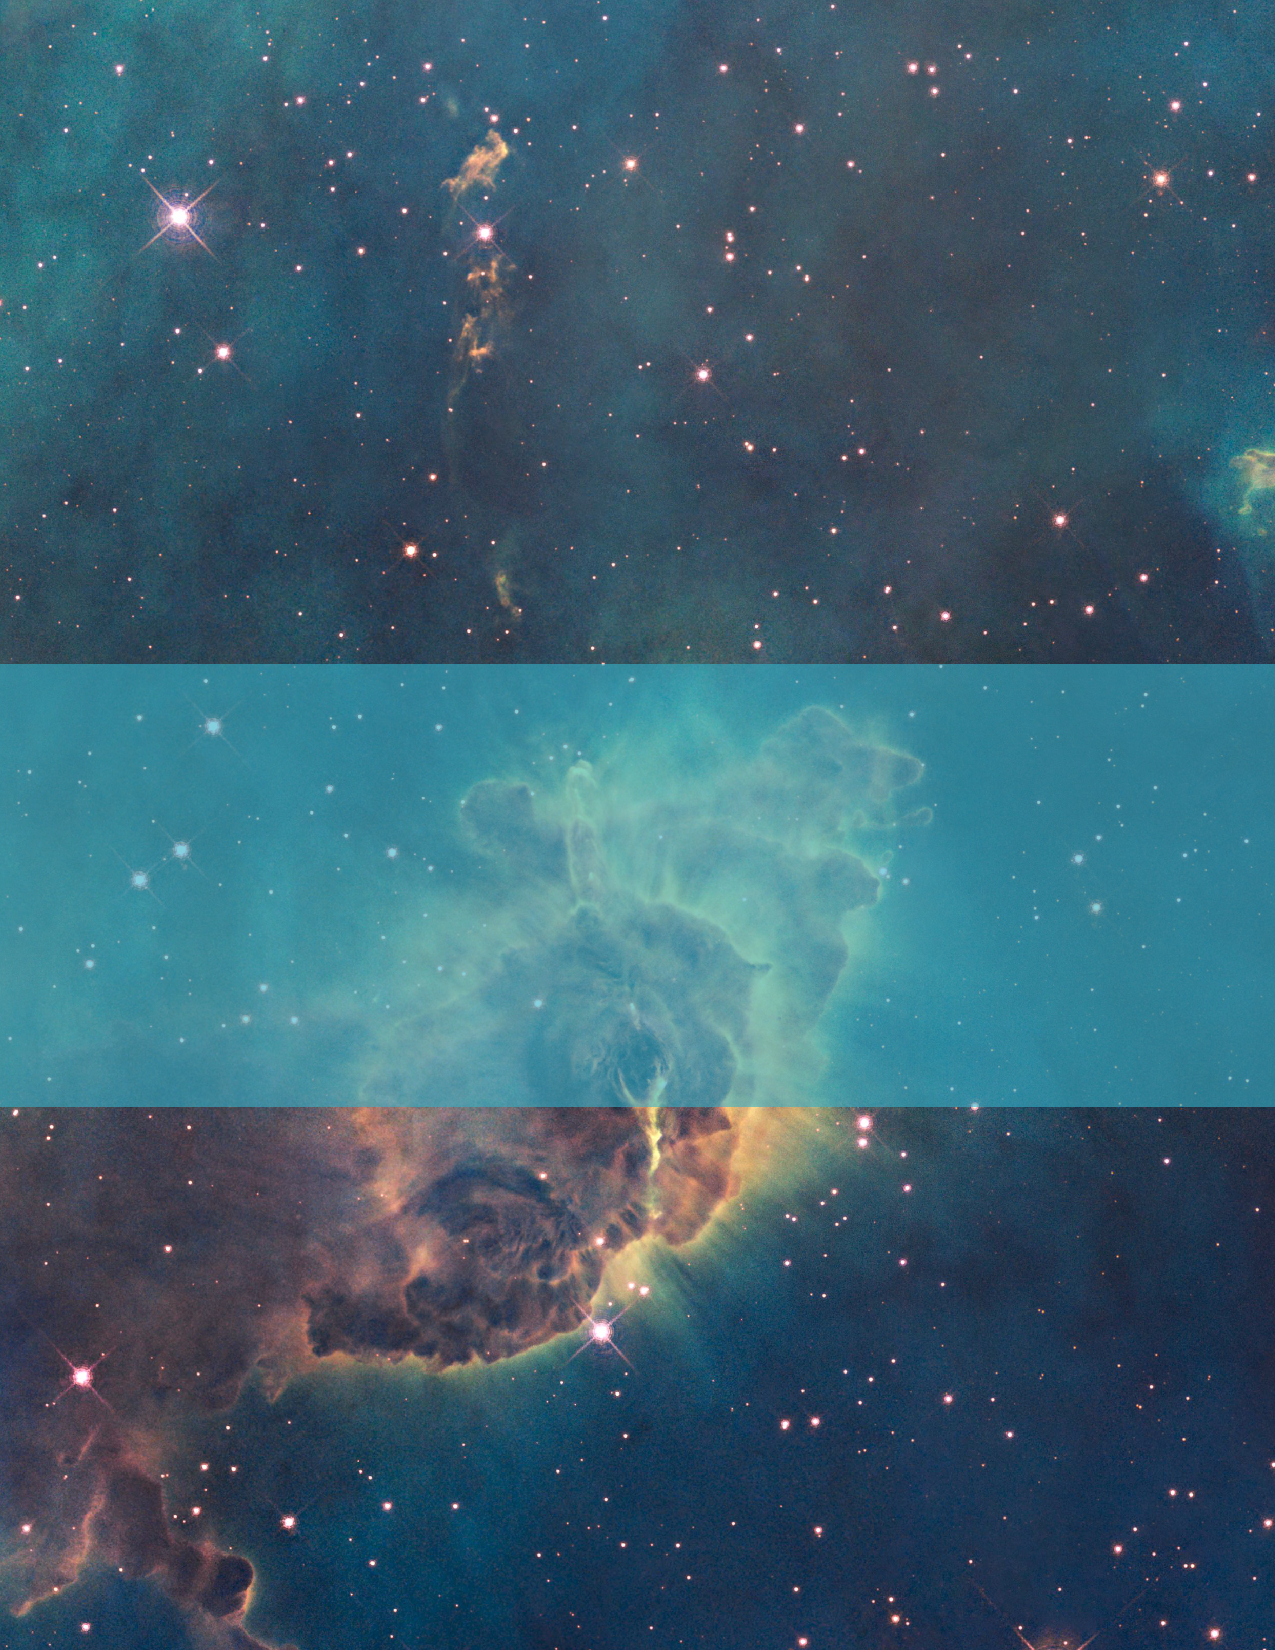
\includegraphics[scale=1.25]{esahubble}}}
\centering
\vspace*{5cm}
\par\normalfont\fontsize{35}{35}\sffamily\selectfont
\textbf{DTU  02501 SPRING 2025}\\
{\LARGE Advanced Deep Learning in Computer Vision}\par
\vspace*{1cm}
{\Huge Lecture Notes}\par
\end{titlepage}
\pagestyle{empty}
\tableofcontents
\clearpage
\pagestyle{fancy}
%----------------------------------------------------------------------------------------
%	TABLE OF CONTENTS
%----------------------------------------------------------------------------------------

%\chapterimage{head1.png} % Table of contents heading image

%\pagestyle{empty} % No headers

%\tableofcontents % Print the table of contents itself

%\cleardoublepage % Forces the first chapter to start on an odd page so it's on the right

%\pagestyle{fancy} % Print headers again

%----------------------------------------------------------------------------------------
%	CHAPTER 1
%----------------------------------------------------------------------------------------
\chapterimage{head2.png} % Chapter heading image
\chapter{\normalsize Lecture 1: Transformers, Attention and Encoders}



\section{Sequence-to-Sequence Models \& Limitations of RNNs}

\subsection*{RNNs limitations (critical to understand):}
\begin{itemize}
    \item Cannot be trained in parallel (sequential processing)
    \item Past information influence is quickly lost over time
    \item Difficult to train due to vanishing/exploding gradients
    \item Formula chain for backpropagation:
    \[
    \frac{\partial h_t}{\partial h_0} = \left(\frac{\partial h_t}{\partial h_{t-1}}\right) \left(\frac{\partial h_{t-1}}{\partial h_{t-2}}\right) \cdots \left(\frac{\partial h_1}{\partial h_0}\right)
    \]
\end{itemize}


\section{Transformer Architecture}

\subsection*{Core innovation:}
Relies entirely on attention mechanisms without recurrence or convolutions

\subsection*{Structure:}
Encoder-Decoder architecture with multiple identical layers

\subsection*{Key components:}
\begin{itemize}
    \item Self-attention mechanism
    \item Multi-head attention
    \item Positional encoding
    \item Feed-forward networks
    \item Add \& Norm (residual connections + layer normalization)
\end{itemize}

\section{Self-Attention Mechanism}

\subsection*{Key equation:}
\[
\text{Attention}(Q, K, V) = \text{softmax}\left(\frac{QK^T}{\sqrt{d_k}}\right)V
\]

\subsection*{Components:}
\begin{itemize}
    \item \textbf{Q (Query)}: What we're looking for
    \item \textbf{K (Key)}: What we match against
    \item \textbf{V (Value)}: What we retrieve
\end{itemize}

\subsection*{Properties:}
Permutation-equivariant (needs positional encoding for order)

\begin{example}
\begin{quote}
\textit{"The animal didn't cross the street because it was too tired,"} self-attention helps \textbf{"it"} attend to \textbf{"animal"}
\end{quote}
\end{example}

\section{Multi-Head Attention}

\subsection*{Purpose:}
Allows the model to jointly attend to information from different representation subspaces

\subsection*{Process:}
\begin{enumerate}
    \item Project input into multiple sets of Q, K, V
    \item Perform attention on each set independently
    \item Concatenate results and project back to original dimension
\end{enumerate}

\subsection*{Formula:}
\[
\text{MultiHead}(Q, K, V) = \text{Concat}(\text{head}_1, \ldots, \text{head}_h) W^O
\]
\[
\text{where head}_i = \text{Attention}(Q W_i^Q, K W_i^K, V W_i^V)
\]

\section{Positional Encoding}

\subsection*{Purpose:}
Add sequence order information since transformer processes tokens in parallel

\subsection*{Original implementation:}
\begin{itemize}
    \item $\text{PE(pos, 2i)} = \sin\left(\frac{\text{pos}}{10000^{\frac{2i}{d_{\text{model}}}}}\right)$
    \item $\text{PE(pos, 2i+1)} = \cos\left(\frac{\text{pos}}{10000^{\frac{2i}{d_{\text{model}}}}}\right)$
\end{itemize}

\subsection*{Alternative:}
Learnable positional encodings (\texttt{nn.Parameter})

\subsection*{Application:}
Added to input embeddings before feeding to the model

\section{Transformer for Classification}

\subsection*{Architecture modifications:}
\begin{enumerate}
    \item Remove Transformer Decoder
    \item Add pooling at the Encoder output (avgpool or [CLS] token)
    \item Add a simple Linear Layer as ``decoder''
\end{enumerate}

\subsection*{[CLS] token approach:}
Special token that aggregates sequence information through self-attention


\section{BERT Overview}

\begin{itemize}
    \item \textbf{Full name:} Bidirectional Encoder Representations from Transformers
    \item \textbf{Pre-training tasks:}
    \begin{itemize}
        \item Masked Language Modeling (MLM)
        \item Next Sentence Prediction (NSP)
    \end{itemize}
    \item \textbf{Fine-tuning:} Add task-specific layers for classification, NER, etc.
\end{itemize}

\section*{Visual Explanations \& Examples to Remember}

\begin{enumerate}
    \item \textbf{YouTube Search as Q-K-V analogy:}
    \begin{itemize}
        \item Query: What you type in search bar
        \item Keys: Video metadata in database
        \item Values: The videos themselves
    \end{itemize}
    
    \item \textbf{Self-attention visualization} showing how words relate to each other:
    \begin{quote}
        Example: "The animal didn't cross the street because it was too tired" where \textbf{"it"} strongly attends to \textbf{"animal"}
    \end{quote}
    
    \item \textbf{Positional encoding heatmap:} Shows sine/cosine patterns that encode position information
\end{enumerate}

\section*{Key Connections to Emphasize}

\begin{enumerate}
    \item \textbf{RNNs $\rightarrow$ Transformers:} Transformers solve RNN limitations by replacing sequential processing with parallel attention
    \item \textbf{Self-attention $\rightarrow$ Multi-head attention:} Multi-head allows model to focus on different aspects of input simultaneously
    \item \textbf{Transformer $\rightarrow$ BERT:} BERT is essentially a pre-trained transformer encoder with specific training objectives
    \item \textbf{Attention $\rightarrow$ Classification:} How self-attention allows aggregation of information for classification tasks
\end{enumerate}

\section*{Quiz Questions for Self-Testing}

\begin{enumerate}
    \item \textbf{Q:} What is the primary advantage of transformer architecture over RNNs?\\
    \textbf{A:} Parallel processing of input sequences, allowing for more efficient training and better capture of long-range dependencies.

    \item \textbf{Q:} Why do we divide by $\sqrt{d_k}$ in the attention formula?\\
    \textbf{A:} To prevent the dot products from growing too large in magnitude, which would lead to extremely small gradients during backpropagation.

    \item \textbf{Q:} Explain the difference between "permutation-equivariant" and "permutation-invariant".\\
    \textbf{A:} Permutation-equivariant means the output changes in a corresponding way when the input order changes. Permutation-invariant means the output remains the same regardless of input order. Self-attention is permutation-equivariant.

    \item \textbf{Q:} Why is positional encoding necessary in transformers?\\
    \textbf{A:} Since transformers process all tokens in parallel with self-attention (which is permutation-equivariant), they need positional encoding to capture sequence order information.

    \item \textbf{Q:} How does the [CLS] token approach differ from average pooling for classification?\\
    \textbf{A:} The [CLS] token learns to aggregate sequence information through self-attention, while average pooling simply takes the mean of all token representations.

    \item \textbf{Q:} What are the components of a typical transformer encoder layer?\\
    \textbf{A:} Multi-head self-attention, Add \& Norm (residual connection and layer normalization), Feed-forward network, and another Add \& Norm.
\end{enumerate}

\vspace{1em}

\section*{Often Overlooked Details Examiners May Ask About}

\begin{enumerate}
    \item \textbf{Scaling factor in attention:} The $\sqrt{d_k}$ term is crucial for gradient stability and often overlooked.

    \item \textbf{Feed-forward networks in transformers:} These are applied position-wise and typically expand dimension then contract:
    \[
    \text{FFN}(x) = \max(0, xW_1 + b_1)W_2 + b_2
    \]

    \item \textbf{Masked self-attention in decoder:} Ensures predictions only depend on known outputs during training.

    \item \textbf{Implementation of multi-head attention:} Involves splitting dimensions rather than separate passes through the attention mechanism.

    \item \textbf{Residual connections:} Critical for training deep transformer networks by helping gradient flow.

    \item \textbf{Layer normalization vs. batch normalization:} Transformers use layer norm which normalizes across features rather than batch examples.

    \item \textbf{Computational complexity of self-attention:} $\mathcal{O}(n^2d)$ where $n$ is sequence length and $d$ is embedding dimension – quadratic in sequence length.
\end{enumerate}

\textbf{Note:} Examiners often ask you to derive or explain the attention mechanism in detail, so be prepared to write out the formula and explain each component's purpose!


\chapterimage{head2.png} % Chapter heading image
\chapter{\normalsize Lecture 2: Visual Transformers}

\section{Foundational Concepts}

\subsection*{Evolution from NLP to Vision}
\begin{itemize}
    \item \textbf{Original Transformer (2017):} \textit{"Attention is All You Need"} paper – revolutionized NLP
    \item \textbf{Key insight:} "An image is worth 16$\times$16 words" – treating image patches as tokens
    \item \textbf{Paradigm shift:} Moving from convolution-based architectures to attention-based ones
    \item \textbf{Main advantage:} Global receptive field from the start (vs. CNNs' local receptive fields)
\end{itemize}

\subsection*{Core Differences: NLP vs. Vision Transformers}

\begin{center}
\begin{tabular}{|l|l|l|}
\hline
\textbf{Aspect} & \textbf{NLP Transformers} & \textbf{Vision Transformers} \\
\hline
Input & 1D sequence of word tokens & 2D grid of pixels converted to patch tokens \\
\hline
Positional encoding & 1D sequence positions & 2D spatial positions (learned, not sinusoidal) \\
\hline
Scale challenges & Hundreds/thousands of tokens & High-resolution images $\rightarrow$ millions of pixels \\
\hline
Inductive bias & Minimal language structure bias & No built-in spatial locality (unlike CNNs) \\
\hline
Data requirements & Moderate & Higher (to compensate for lack of inductive bias) \\
\hline
\end{tabular}
\end{center}

\section{Vision Transformer (ViT) Architecture}

\subsection*{Input Processing Pipeline}
\begin{enumerate}
    \item \textbf{Patch extraction:} Divide image into non-overlapping patches (typically 16$\times$16 pixels)
    \item \textbf{Linear projection:} Flatten patches and project to embedding dimension (D)
    \item \textbf{Class token:} Add learnable [CLS] token for classification (like BERT)
    \item \textbf{Positional embedding:} Add learned positional embeddings to retain spatial information
\end{enumerate}

\subsection*{Core Components}
\begin{itemize}
    \item \textbf{Transformer Encoder:} Series of Multi-Head Self-Attention layers and MLPs
    \item \textbf{Self-Attention:} Same mechanism as in NLP transformers
    \item \textbf{MLP Head:} Final classification layer applied to [CLS] token output
\end{itemize}

\subsection*{ViT Variants and Scaling}
\begin{itemize}
    \item \textbf{Size variants:} Base (L=12, H=768), Large (L=24, H=1024), Huge (L=32, H=1280)
    \item \textbf{Training efficiency:} ViT with 2.5k TPU days outperforms ResNet with 9.9k TPU days
    \item \textbf{Patch size impact:} Smaller patches $\rightarrow$ more tokens $\rightarrow$ higher computational cost but better performance
\end{itemize}
\section{Hierarchical Vision Transformers}

\subsection*{Swin Transformer}
\begin{itemize}
    \item \textbf{Key innovation:} Hierarchical structure with shifted windows of attention
    \item \textbf{Window-based attention:} Compute self-attention within local windows to reduce complexity
    \item \textbf{Shifting windows:} Alternate layers shift attention windows to enable cross-window connections
    \item \textbf{Progressive downsampling:} Merge neighboring patches to create hierarchical representation
    \item \textbf{Complexity:} Linear complexity with image size (vs. quadratic in vanilla ViT)
\end{itemize}

\subsection*{Advantages}
\begin{itemize}
    \item \textbf{Efficiency:} $\mathcal{O}(n)$ complexity vs. $\mathcal{O}(n^2)$ in vanilla transformers
    \item \textbf{Multi-scale processing:} Better suited for dense prediction tasks (detection, segmentation)
    \item \textbf{Performance:} Strong results with less computational resources
\end{itemize}

\section{Object Detection with Transformers}

\subsection*{DETR (DEtection TRansformer)}
\textbf{End-to-end approach:} No need for hand-designed components like anchors and NMS

\subsection*{Architecture}
\begin{enumerate}
    \item CNN backbone extracts features
    \item Transformer encoder processes these features
    \item Transformer decoder with object queries predicts boxes directly
    \item Feed-forward networks convert query outputs to box coordinates and class labels
\end{enumerate}

\subsection*{Bipartite Matching Loss}
\begin{itemize}
    \item \textbf{Key innovation:} One-to-one assignment between predictions and ground truth
    \item \textbf{Contrast with traditional methods:} Traditional detectors use one-to-many assignment with NMS
    \item \textbf{Implementation:} Hungarian algorithm to find optimal matching
    \item \textbf{Training formulation:} Predefined number of queries (N) matched to ground truth boxes plus ``no object'' fillers
\end{itemize}

\subsection*{Benefits}
\begin{itemize}
    \item \textbf{Simplified pipeline:} Direct set prediction without post-processing
    \item \textbf{Global reasoning:} Objects predicted in relation to each other
    \item \textbf{Parallel decoding:} All objects predicted simultaneously
\end{itemize}

\section{Image Segmentation with Transformers}

\subsection*{Key Architectures}
\begin{itemize}
    \item \textbf{SETR:} Encoder-only approach with CNN decoder for upsampling
    \item \textbf{SegFormer:} Efficient hierarchical design with lightweight decoder
    \item \textbf{MaskFormer:} Query-based approach with mask predictions (treats segmentation as mask classification)
    \item \textbf{Mask2Former:} Improved MaskFormer with masked attention mechanism
\end{itemize}

\subsection*{Common Principles}
\begin{itemize}
    \item \textbf{Global context:} Transformers capture long-range dependencies important for segmentation
    \item \textbf{Query-based formulation:} Moving from per-pixel classification to mask prediction
    \item \textbf{Unified approach:} Same architecture works for semantic, instance, and panoptic segmentation
\end{itemize}

\section{Advanced Concepts}

\subsection*{Positional Encoding in Vision}
\begin{itemize}
    \item \textbf{Learned 1D embeddings:} Despite dealing with 2D images, ViT uses 1D position embeddings
    \item \textbf{Emergent properties:} Position embeddings learn to encode:
    \begin{itemize}
        \item Distance (closer patches $\rightarrow$ similar embedding)
        \item Row/column structure (patches in same row/col have similar embeddings)
        \item 2D image topology (despite only being trained with 1D sequence)
    \end{itemize}
\end{itemize}

\subsection*{Attention Visualization and Interpretability}
\begin{itemize}
    \item \textbf{Attention rollout:} Method to visualize attention flow through multiple layers
    \item \textbf{Last layer attention:} Shows which patches are most relevant for classification
    \item \textbf{Visual examples:} Shows transformers attend to semantically meaningful parts of images
\end{itemize}

\subsection*{Memory and Computational Challenges}
\begin{itemize}
    \item \textbf{Full self-attention:} $\mathcal{O}(n^2)$ complexity is problematic for high-resolution images
    \item \textbf{Strategies to address:}
    \begin{enumerate}
        \item Window-based attention (Swin)
        \item Hierarchical architectures
        \item Linear attention approximations
        \item Hybrid CNN-Transformer architectures
    \end{enumerate}
\end{itemize}
\section{Quiz Questions with Answers}

\begin{enumerate}
    \item \textbf{Q:} What is the fundamental difference in how ViT processes images compared to CNNs?\\
    \textbf{A:} ViT splits images into patches and processes them as a sequence using self-attention, whereas CNNs use local convolution operations with increasing receptive fields through the network.

    \item \textbf{Q:} Why do Vision Transformers typically require more training data than CNNs?\\
    \textbf{A:} Vision Transformers lack the inductive biases of CNNs (locality, translation equivariance) and must learn these relationships from data, requiring more examples to generalize well.

    \item \textbf{Q:} Explain the purpose of the [CLS] token in Vision Transformers.\\
    \textbf{A:} The [CLS] token is a learnable embedding prepended to the sequence of patch embeddings. Through self-attention, it aggregates information from all patches, and its final representation is used for image classification.

    \item \textbf{Q:} How does the bipartite matching loss in DETR eliminate the need for NMS?\\
    \textbf{A:} Bipartite matching creates a one-to-one assignment between predictions and ground truth objects, forcing the model to output exactly one prediction per object. This inherently avoids duplicate detections, making NMS unnecessary.

    \item \textbf{Q:} What is the key innovation of Swin Transformer that addresses the computational complexity of ViT?\\
    \textbf{A:} Swin Transformer computes self-attention within local windows rather than globally, reducing complexity from $\mathcal{O}(n^2)$ to $\mathcal{O}(n)$. It also uses shifted window patterns between layers to allow information flow across windows.

    \item \textbf{Q:} How does MaskFormer change the approach to semantic segmentation compared to traditional methods?\\
    \textbf{A:} MaskFormer reformulates semantic segmentation from per-pixel classification to a set prediction problem, where the model predicts masks with associated class labels, similar to DETR's approach to object detection.
\end{enumerate}

\chapterimage{head2.png} % Chapter heading image
\chapter{\normalsize Lecture 3: Transformer Decoders, LLMs and GPTs}


\subsubsection*{Transformer Architecture Overview}
\begin{itemize}
    \item \textbf{Transformer Decoder:} The component responsible for generating output sequences token by token
    \item \textbf{Essential Components:}
    \begin{enumerate}
        \item Masked Multi-Head Attention (enforces autoregressive property)
        \item Multi-Head Cross-Attention (connects to encoder if present)
        \item Feed-Forward Networks
        \item Layer Normalization
        \item Residual connections
    \end{enumerate}
\end{itemize}

\subsubsection*{Key Transformer Model Types}
\begin{itemize}
    \item \textbf{Encoder-Decoder Models:} Translation, summarization (original Transformer)
    \item \textbf{Encoder-Only Models:} BERT, text classification, understanding
    \item \textbf{Decoder-Only Models:} GPT family, text generation, most modern LLMs
\end{itemize}

\subsubsection*{Attention Mechanisms}
\begin{itemize}
    \item \textbf{Self-Attention:} Token relationships within the same sequence
    \item \textbf{Masked Self-Attention:} Only allows a token to attend to previous tokens (slides 24--25)
    \item \textbf{Cross-Attention:} Allows decoder to attend to encoder outputs (slide 26)
    \item \textbf{Multi-Head Attention:} Allows multiple attention patterns in parallel
\end{itemize}

\subsubsection*{Autoregressive Generation (Critical for GPT-style models)}
\begin{itemize}
    \item Tokens generated sequentially, with each new token conditioned on all previous tokens
    \item \textbf{Formula:}
    \[
    P(w_1, w_2, \dots, w_n) = \prod_{i} P(w_i \mid w_1, w_2, \dots, w_{i-1})
    \]
    \item Enforced via \textbf{causal masking} in the attention mechanism
\end{itemize}
\section{GPT-Style Models vs BERT}

\subsection*{GPT Architecture \& Function}
\begin{itemize}
    \item \textbf{Decoder-only} transformer model
    \item \textbf{Unidirectional} (left-to-right) attention
    \item \textbf{Autoregressive} next token prediction
    \item Trained using standard language modeling objective
    \item Generate text by sampling from conditional probability distributions
\end{itemize}

\subsection*{BERT vs. GPT Comparison (Slide 32--33)}
\begin{center}
\begin{tabular}{|l|l|l|}
\hline
\textbf{Feature} & \textbf{BERT} & \textbf{GPT} \\
\hline
Model Type & Encoder-Only & Decoder-Only \\
\hline
Direction & Bidirectional & Unidirectional (left-to-right) \\
\hline
Pre-training & Masked Language Modeling (MLM) & Autoregressive Language Modeling \\
\hline
Fine-tuning & Task-specific layer added on top & Few-shot prompting or fine-tuning \\
\hline
Use Case & Understanding (classification, NER) & Generation (text completion, creative writing) \\
\hline
Original Creator & Google AI & OpenAI \\
\hline
\end{tabular}
\end{center}

\subsection*{Training Objectives}
\begin{itemize}
    \item \textbf{GPT:} Predict next token given previous tokens
    \item \textbf{BERT:} Predict masked tokens using bidirectional context
\end{itemize}
\section{Machine Translation with Transformers}

\subsection*{Encoder-Decoder for Translation}
\begin{itemize}
    \item \textbf{Input:} Source language sequence processed by encoder
    \item \textbf{Output:} Target language sequence generated by decoder
    \item \textbf{Cross-attention:} Decoder queries attend to encoder key-value pairs
    \item \textbf{Training objective:} Teacher forcing with target sequence
\end{itemize}

\subsection*{Translation Process (From Slides 12--23)}
\begin{enumerate}
    \item Source sentence tokenized and fed to encoder
    \item Encoder builds contextual representations
    \item Decoder starts with special start token
    \item Decoder generates target tokens one-by-one
    \item Cross-attention allows decoder to focus on relevant source tokens
    \item Process continues until end token is generated
\end{enumerate}

\subsection*{Difference from Decoder-Only Models}
\begin{itemize}
    \item Encoder-decoder has explicit source encoding step
    \item Cross-attention mechanism connects source and target
    \item More parameter-efficient for translation tasks
    \item Better handling of source language nuances
\end{itemize}
\section{Key Diagrams \& Workflows}

\subsection*{Transformer Decoder Structure (Slide 24)}
The presentation shows the decoder with:
\begin{itemize}
    \item Masked Multi-Head Attention block
    \item Multi-Head Cross-Attention block (for encoder-decoder models)
    \item Feed-Forward Networks
    \item Layer normalization and residual connections
\end{itemize}

\subsection*{Masked Attention Mechanism (Slide 25)}
\begin{itemize}
    \item Shows how attention is masked to prevent looking at future tokens
    \item Contrast between standard self-attention and masked self-attention
    \item Implementation by setting future position scores to negative infinity
\end{itemize}

\subsection*{Autoregressive Decoder Workflow (Slides 17--22)}
\begin{itemize}
    \item Step-by-step illustration of how tokens are generated
    \item Starts with special token \texttt{<START>}
    \item Generates one token at a time
    \item Each new token depends on all previous tokens
\end{itemize}

\subsection*{Decoding Strategies (Slides 40--47)}
\begin{itemize}
    \item \textbf{Greedy decoding:} Always select highest probability token
    \item \textbf{Beam search:} Maintain multiple hypotheses
    \item \textbf{Sampling:} Draw from probability distribution (with temperature control)
\end{itemize}
\section{Practice Quiz Questions}

\begin{enumerate}
    \item \textbf{Q:} What is the key difference between the attention mechanism in BERT and GPT?\\
    \textbf{A:} BERT uses bidirectional self-attention, while GPT uses masked (causal) self-attention that only allows a token to attend to previous tokens.

    \item \textbf{Q:} Why can't GPT process all output tokens in parallel during inference?\\
    \textbf{A:} Due to the autoregressive nature, each token depends on previously generated tokens, forcing sequential generation.

    \item \textbf{Q:} What is the purpose of cross-attention in an encoder-decoder transformer?\\
    \textbf{A:} Cross-attention allows the decoder to attend to relevant parts of the encoder's output, connecting source and target sequences.

    \item \textbf{Q:} How does beam search differ from greedy decoding?\\
    \textbf{A:} Greedy decoding selects the most probable token at each step, while beam search maintains multiple hypotheses and selects the overall most probable sequence.

    \item \textbf{Q:} Why might multinomial sampling with temperature control produce more diverse text than beam search?\\
    \textbf{A:} Sampling introduces randomness that helps avoid repetitive patterns, while temperature control allows balancing between diversity and coherence.

    \item \textbf{Q:} What problem in tokenization does Byte Pair Encoding (BPE) address?\\
    \textbf{A:} BPE balances vocabulary size and sequence length by using subword units, handling rare words better than word-level tokenization while being more efficient than character-level tokenization.
\end{enumerate}
\section{Common Pitfalls \& Advanced Questions}

\subsection*{Causal Masking in GPT}
\begin{itemize}
    \item \textbf{Mechanism:} Sets attention scores for future positions to negative infinity
    \item \textbf{Purpose:} Enforces autoregressive constraint
    \item \textbf{Pitfall:} Confusing with padding masks (different purpose)
    \item \textbf{Examiner might ask:} How does causal masking contribute to the training efficiency of GPT models?
\end{itemize}

\subsection*{Parallel Processing Limitations}
\begin{itemize}
    \item \textbf{Training:} Can be parallelized because ground truth is available
    \item \textbf{Inference:} Must be sequential due to autoregressive nature
    \item \textbf{Pitfall:} Assuming inference can be parallelized like training
    \item \textbf{Examiner might ask:} What approaches might improve inference speed in autoregressive models?
\end{itemize}

\subsection*{Long-Range Dependencies}
\begin{itemize}
    \item \textbf{Challenge:} Attention complexity grows quadratically with sequence length
    \item \textbf{Solutions:} Sparse attention, sliding windows, hierarchical attention
    \item \textbf{Pitfall:} Not understanding the computational bottlenecks
    \item \textbf{Examiner might ask:} How do modern LLMs handle context windows of 100K+ tokens?
\end{itemize}

\subsection*{Tokenization Tradeoffs}
\begin{itemize}
    \item \textbf{Character-level:} Small vocabulary, long sequences
    \item \textbf{Word-level:} Large vocabulary, OOV problems
    \item \textbf{Subword (BPE):} Compromise, $\sim$4 characters per token in English
    \item \textbf{Examiner might ask:} How might tokenization biases affect model performance across languages?
\end{itemize}

\subsection*{Decoding Strategy Selection}
\begin{itemize}
    \item \textbf{When to use beam search:} When the most probable overall sequence is desired
    \item \textbf{When to use sampling:} When diversity is important
    \item \textbf{Pitfall:} Using the wrong strategy for the application
    \item \textbf{Examiner might ask:} Why does beam search tend to produce repetitive text in open-ended generation?
\end{itemize}

\subsection*{Evaluation Challenges}
\begin{itemize}
    \item \textbf{Automated metrics:} BLEU, ROUGE have limitations
    \item \textbf{Human evaluation:} Subjective but often necessary
    \item \textbf{Pitfall:} Over-reliance on automated metrics
    \item \textbf{Examiner might ask:} How would you evaluate an LLM for factual accuracy versus creativity?
\end{itemize}

\chapterimage{head2.png} % Chapter heading image
\chapter{\normalsize Lecture notes: Diffusion Models}


\subsection*{1. Fundamental Concepts of Diffusion Models}

Diffusion models belong to the class of generative models --- models that describe a probability distribution $p$ and can generate samples from that distribution. They joined other generative approaches like Variational Autoencoders (VAEs), normalizing flows, and Generative Adversarial Networks (GANs).

Denoising Diffusion Probabilistic Models (DDPMs) were introduced in the paper by Ho et al.~[4]. Until their arrival, GANs were the dominant approach for high-quality image generation, despite being less probabilistically rigorous. DDPMs have since surpassed GANs in visual quality.

\subsection*{Key Differentiators from Other Generative Models}

In traditional generative models like VAEs and GANs, we learn to predict data (images) from latent vectors that follow a predefined distribution (often Gaussian). Diffusion models encode images differently --- by incrementally adding noise to the image over a pre-determined number ($T$) of time steps.

Two crucial differences from VAEs/GANs:
\begin{enumerate}
    \item \textbf{No dimension reduction} --- There is no inherent dimension reduction in the latent representations.
    \item \textbf{No semantic structure} --- The Step 0 latent representation contains no semantic or geometric information. Interpolating between two noised images will not generate semantically meaningful transformations.
\end{enumerate}

\section{The Forward Process (Diffusion/Noise Addition)}

The forward process is formalized as a Markov process $q$ that progressively adds noise to an image:
\begin{definition}[Forward Process of Diffusion Model]
\[
q(x_{1:T} \mid x_0) := \prod_{t=1}^{T} q(x_t \mid x_{t-1})
\]
where
\[
q(x_t \mid x_{t-1}) := \mathcal{N}(x_t; \sqrt{1 - \beta_t}x_{t-1}, \beta_t \mathbf{I})
\]
\end{definition}

Here, $\mathbf{I}$ is the identity covariance matrix over image space, and $\beta_t$ values are hyperparameters referred to as the variance schedule.

\subsection*{Closed-form Sampling}
A key insight is that we can derive a closed-form expression to directly sample a noisy image at any time step without having to sequentially add noise:
\begin{definition}[Closed form sampling]
\[
q(x_t \mid x_0) = \mathcal{N}(x_t; \sqrt{\bar{\alpha}_t} x_0, (1 - \bar{\alpha}_t)\mathbf{I})
\]
where $\alpha_t := 1 - \beta_t$ and $\bar{\alpha}_t := \prod_{s=1}^{t} \alpha_s$.
\end{definition}

\subsection*{Variance Scheduling}
For implementation, the original DDPM paper uses a linear variance schedule with $\beta_t$ increasing from $\beta_1 = 10^{-4}$ to $\beta_T = 0.02$. Alternative schedules like the cosine schedule have also been proposed, which emphasize later denoising steps.

\section{The Reverse Process (Denoising)}

The reverse process is where the main work happens --- the DDPM learns to generate noise-free images from their noisy representations. This iterative denoising is performed by a deep neural network that represents a joint distribution $p_\theta(x_{0:T})$.

\begin{definition}[Reverse Process (Denoising)]
Like the forward process, the reverse process is a Markov chain:
\[
p_\theta(x_{0:T}) := p(x_T) \prod_{t=1}^{T} p_\theta(x_{t-1} \mid x_t)
\]
where
\[
p_\theta(x_{t-1} \mid x_t) = \mathcal{N}(x_{t-1}; \mu_\theta(x_t, t), \Sigma_\theta(x_t, t))
\]

The process typically starts with an initial noise image $x_T$ drawn from a standard normal distribution:
\[
p(x_T) = \mathcal{N}(x_T; 0, \mathbf{I})
\]
\end{definition}

\section{Learning to Denoise}

Rather than predicting the denoised image $x_{t-1}$ directly from $x_t$, empirical research has found it easier to predict the noise $\epsilon$ that was used to generate $x_t$ from the original noise-free image $x_0$.

\subsection*{Reparameterized Forward Equation}
This uses the formula:
\begin{definition}[Reparametrization Trick]
\[
x_t = \sqrt{\bar{\alpha}_t} x_0 + \sqrt{1 - \bar{\alpha}_t} \, \epsilon
\]
The model is trained to predict $\epsilon_\theta(x_t, t)$, which estimates the noise $\epsilon$ from $x_t$.
\end{definition}

\subsection*{Architecture}
\begin{itemize}
    \item U-Net architecture is widely used as it's effective for image-to-image tasks
    \item Time point $t$ is included as an additional input
    \item At every down- and upsampling step, time is incorporated as a broadcast channel
    \item This broadcasted time representation is added to the image, similar to positional encoding
\end{itemize}

\subsection*{Loss Function}
The DDPM paper derives a Bayesian loss, but in practice a simpler MSE loss is used:
\begin{definition}[Loss Function]
\[
L_{\text{simple}}(\theta) := \mathbb{E}_{x_0, \epsilon, t} \left[\left\| \epsilon - \epsilon_\theta\left(\sqrt{\bar{\alpha}_t} x_0 + \sqrt{1 - \bar{\alpha}_t} \, \epsilon, t \right) \right\|^2 \right]
\]
\end{definition}
This is simply the mean squared error (MSE) between the predicted noise and the true noise $\epsilon$.

\section{Training and Sampling Process}


\subsection*{Training}
At each training iteration:
\begin{enumerate}
    \item Sample a random $x_0$ from data
    \item Sample a random time point $t$ uniformly from the $T$ time points
    \item Sample random noise $\epsilon \sim \mathcal{N}(0, \mathbf{I})$
    \item Compute the noisy image:
\begin{definition}[Noisy image at time $t$]    \[
    x_t = \sqrt{\bar{\alpha}_t} x_0 + \sqrt{1 - \bar{\alpha}_t} \, \epsilon
    \]\end{definition}
    \item Make a gradient update of the MSE loss w.r.t. $\theta$
\end{enumerate}
\begin{figure}[H]
    \centering
    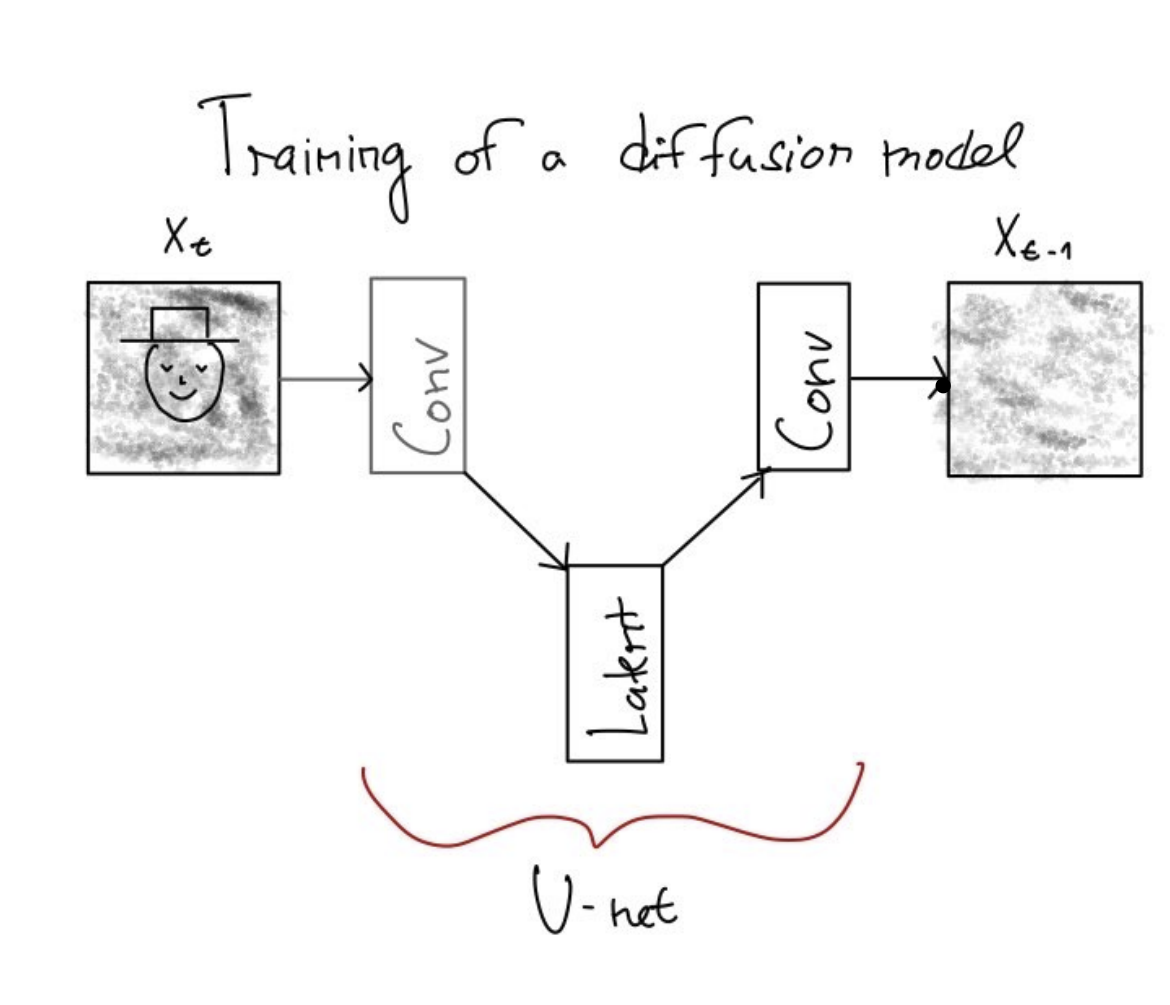
\includegraphics[width=1\linewidth]{billede.png}
    \caption{Illustration of the denoising diffusion process using a U-Net architecture. At each denoising step, the U-Net model $\epsilon_\theta$ predicts the noise component $\epsilon$ present in the noisy image $x_t$. Rather than directly predicting the clean image, the model outputs the estimated noise $\hat{\epsilon}_\theta(x_t, t)$, which is then subtracted from $x_t$ (with appropriate scaling based on the diffusion schedule) to obtain the less noisy image approximation $x_{t-1}$. This approach, where the network is trained to minimize $\mathbb{E}[\|\epsilon - \hat{\epsilon}_\theta(x_t, t)\|^2]$, has been shown to provide more stable training dynamics than directly predicting the denoised image.}
    \label{fig:unet_denoising}
\end{figure}
\subsection*{Sampling}
For sampling from the model:
\begin{enumerate}
    \item Set covariance $\Sigma_\theta(x_t, t) = \sigma_t^2 \mathbf{I}$, where $\sigma_t^2 = \beta_t$ (simplest version)
    \item Set mean:
    \begin{definition}[Denoising Mean Equation:]

    
    \[
    \mu_\theta(x_t, t) = \frac{1}{\sqrt{\alpha_t}} \left(x_t - \frac{\beta_t}{\sqrt{1 - \bar{\alpha}_t}} \epsilon_\theta(x_t, t)\right)
    \]
    \end{definition}
    \item Sample $x_{t-1} \sim \mathcal{N}(\mu_\theta, \Sigma_\theta)$
    \item Repeat iteratively to sample $x_{t-1}$ from $x_T$
\end{enumerate}



\section{Key Exam Topics and Common Questions}

\subsection*{What makes diffusion models different from VAEs and GANs?}
\begin{itemize}
    \item No dimension reduction in latent space
    \item Latent variables have no semantic structure
    \item Progressive noise addition/removal rather than direct encoding/decoding
    \item More stable training compared to GANs
    \item Better image quality than earlier models
\end{itemize}

\subsection*{What is the variance schedule $\beta_1 \ldots \beta_T$ and why is it important?}
\begin{itemize}
    \item Controls how quickly noise is added in the forward process
    \item Affects the difficulty of the denoising task
    \item Different schedules (linear, cosine) have different properties
    \item Cosine schedule focuses learning more on later denoising steps
\end{itemize}

\subsection*{Why do we predict noise $\epsilon$ rather than directly predicting $x_{t-1}$?}
\begin{itemize}
    \item Empirically proven to be easier and more effective
    \item Allows for a simpler loss function (MSE)
    \item Results in better performance
\end{itemize}

\subsection*{What architecture is typically used for diffusion models?}
\begin{itemize}
    \item U-Net architecture (originally designed for image segmentation)
    \item Modified to incorporate time as an additional input
    \item Time is broadcast as a channel and added at each scale
\end{itemize}

\subsection*{How is the sampling process defined in diffusion models?}
\begin{itemize}
    \item Start with pure noise $x_T \sim \mathcal{N}(0, \mathbf{I})$
    \item Iteratively denoise step by step using the learned model
    \item Each step involves sampling from a Gaussian with learned parameters
    \item Final result $x_0$ is the generated sample
\end{itemize}


\section{Practice Questions for Exam Preparation}

\begin{enumerate}
    \item \textbf{Q:} Explain the mathematical formulation of the forward process in diffusion models.\\
    \textbf{A:} The forward process is a Markov chain that progressively adds Gaussian noise to an image:
    \[
    q(x_{1:T} \mid x_0) := \prod_{t=1}^{T} q(x_t \mid x_{t-1})
    \quad \text{where} \quad q(x_t \mid x_{t-1}) := \mathcal{N}(x_t; \sqrt{1 - \beta_t} x_{t-1}, \beta_t \mathbf{I})
    \]
    This can be reparameterized to directly sample $x_t$ from $x_0$:
    \[
    q(x_t \mid x_0) = \mathcal{N}(x_t; \sqrt{\bar{\alpha}_t} x_0, (1 - \bar{\alpha}_t) \mathbf{I})
    \]

    \item \textbf{Q:} What is being learned by the neural network in a DDPM?\\
    \textbf{A:} The neural network is learning to predict the noise $\epsilon$ that was added to the original image, given a noisy image $x_t$ and time step $t$. This is then used to construct the parameters (mean and variance) of the reverse process distributions.

    \item \textbf{Q:} Why is the U-Net architecture suitable for diffusion models?\\
    \textbf{A:} The U-Net is designed for image-to-image tasks where spatial relationships matter. It has skip connections that help preserve spatial information. In diffusion models, we’re essentially doing image-to-image tasks: predicting noisy or denoised images with the same dimensions as the input.

    \item \textbf{Q:} How does the training objective differ from the theoretical formulation in the DDPM paper?\\
    \textbf{A:} While the theoretical loss is based on a variational lower bound, in practice a simpler MSE loss is used between the predicted noise and the actual noise. This was found to work better empirically.

    \item \textbf{Q:} What extensions to diffusion models might be covered in the next lecture?\\
    \textbf{A:} The next lecture will cover conditioning and guidance techniques, including classifier guidance, classifier-free guidance, universal guidance, and counterfactual explanations via diffusion models.
\end{enumerate}

\section{Common Pitfalls and Deep Insights}

\begin{itemize}
    \item \textbf{Latent Space Structure:} Unlike VAEs, the latent space in diffusion models lacks semantic structure, so traditional interpolation doesn’t work for tasks like “making a person smile.”

    \item \textbf{Computational Cost:} Diffusion models require sequential sampling through $T$ steps, making them slower than single-pass generators like GANs.

    \item \textbf{Theoretical vs. Practical:} There’s often a gap between theory and what works best in practice (e.g., simplified MSE loss performs better than variational losses).

    \item \textbf{Hyperparameter Sensitivity:} The variance schedule significantly affects performance and requires careful tuning.

    \item \textbf{Connection to Score-Based Models:} Diffusion models are closely related to score-based generative models – this insight may come up in deeper theoretical discussions.
\end{itemize}

\textbf{Reflection Prompt:} Be prepared to explain how you would approach the task of \textit{“making a person smile”} with a diffusion model, as this was posed as a discussion point in the notes.


\chapterimage{head2.png} % Chapter heading image
\chapter{\normalsize Lecture 4: Diffusion Models}

\section{Overview of Diffusion Models}

Diffusion models generate data by reversing a gradual noising process. Unlike other generative models that map from a fixed latent distribution to data, diffusion models:

\begin{itemize}
    \item Encode images by progressively adding noise over $T$ time steps
    \item Learn to reverse this process by denoising step-by-step
    \item Use noisy images as time-dependent latent variables
\end{itemize}

\subsection*{Key Distinction from Other Generative Models}

Traditional generative models (GANs, VAEs) map latent vectors to data directly. In contrast, diffusion models:

\begin{itemize}
    \item Work with a sequence of increasingly noisy versions of the data
    \item Define both forward (noising) and reverse (denoising) Markov processes
    \item Train a neural network to predict and remove noise at each step
\end{itemize}

\section{The Forward and Reverse Processes}

\subsection*{Forward Process (Adding Noise)}

The forward process is a Markov chain that gradually adds Gaussian noise:

\begin{itemize}
    \item \textbf{Mathematical formulation:}
    \[
    q(x_{1:T} \mid x_0) := \prod_{t=1}^{T} q(x_t \mid x_{t-1}), \quad q(x_t \mid x_{t-1}) := \mathcal{N}(x_t; \sqrt{1 - \beta_t} x_{t-1}, \beta_t \mathbf{I})
    \]
    
    \item \textbf{Variance schedule:} $\beta_1, \beta_2, \dots, \beta_T$ determines noise scaling
    \begin{itemize}
        \item Ho et al. use a linear schedule from $\beta_1 = 10^{-4}$ to $\beta_T = 0.02$
        \item Nichol et al. later improved this with a cosine schedule
    \end{itemize}
    
    \item \textbf{Closed-form sampling:}
    \[
    q(x_t \mid x_0) = \mathcal{N}(x_t; \sqrt{\bar{\alpha}_t} x_0, (1 - \bar{\alpha}_t) \mathbf{I})
    \]
    where $\alpha_t := 1 - \beta_t$ and $\bar{\alpha}_t := \prod_{s=1}^{t} \alpha_s$
    
    \item \textbf{Reparameterization trick:}
    \[
    x_t(x_0, \epsilon) = \sqrt{\bar{\alpha}_t} x_0 + \sqrt{1 - \bar{\alpha}_t} \, \epsilon, \quad \epsilon \sim \mathcal{N}(0, \mathbf{I})
    \]
\end{itemize}

\subsection*{Reverse Process (Generative Process)}

The reverse process is also a Markov chain, but with learned Gaussian transitions:

\begin{itemize}
    \item \textbf{Mathematical formulation:}
    \[
    p_\theta(x_{0:T}) := p(x_T) \prod_{t=1}^{T} p_\theta(x_{t-1} \mid x_t), \quad p_\theta(x_{t-1} \mid x_t) := \mathcal{N}(x_{t-1}; \mu_\theta(x_t, t), \Sigma_\theta(x_t, t))
    \]
    Initialized with $p(x_T) = \mathcal{N}(x_T; 0, \mathbf{I})$
    
    \item \textbf{Key insight:} Instead of predicting $x_{t-1}$ directly, we predict the noise $\epsilon$ that was added
    \begin{itemize}
        \item The model $\epsilon_\theta(x_t, t)$ is trained to estimate $\epsilon$ from the noisy image $x_t$
    \end{itemize}
    
    \item \textbf{Sampling equation:}
    \[
    x_{t-1} = \frac{1}{\sqrt{\alpha_t}} \left( x_t - \frac{1 - \alpha_t}{\sqrt{1 - \bar{\alpha}_t}} \epsilon_\theta(x_t, t) \right) + \sigma_t z
    \]
    Where $\sigma_t = \beta_t$ and $z$ is random noise ($z = 0$ at final step)
\end{itemize}


\section{Model Architecture and Training}

\subsection*{Architecture}
\begin{itemize}
    \item \textbf{U-Net backbone:} The noise predictor $\epsilon_\theta$ uses a U-Net architecture.
    \item \textbf{Time conditioning:} The time step $t$ is an additional input, broadcast and added to the image representation at each layer (similar to positional encoding).
\end{itemize}

\subsection*{Training Objective}
\begin{itemize}
    \item \textbf{Theoretical foundation:} While a variational bound (ELBO) exists, a simpler loss works better in practice.
    \item \textbf{Simplified loss:}
    \[
    L_{\text{simple}}(\theta) := \mathbb{E}_{x_0, \epsilon, t} \left[\left\| \epsilon - \epsilon_\theta\left(\sqrt{\bar{\alpha}_t}x_0 + \sqrt{1 - \bar{\alpha}_t} \, \epsilon, t\right) \right\|^2\right]
    \]
    \item \textbf{Intuition:} The model directly predicts the noise that was added to create $x_t$ from $x_0$.
\end{itemize}

\subsection*{Training Algorithm}
\begin{enumerate}
    \item Sample $x_0$ from the data distribution
    \item Sample a random time step $t \sim \text{Uniform}(\{1, \ldots, T\})$
    \item Sample random noise $\epsilon \sim \mathcal{N}(0, \mathbf{I})$
    \item Create noisy sample: \[
    x_t = \sqrt{\bar{\alpha}_t} x_0 + \sqrt{1 - \bar{\alpha}_t} \, \epsilon
    \]
    \item Train the model to predict $\epsilon$ given $x_t$ and $t$
\end{enumerate}

\subsection*{Sampling/Generation Algorithm}
\begin{enumerate}
    \item Sample $x_T \sim \mathcal{N}(0, \mathbf{I})$ (pure noise)
    \item For $t = T, T-1, \ldots, 1$:
    \begin{itemize}
        \item Sample $z \sim \mathcal{N}(0, \mathbf{I})$ if $t > 1$, else $z = 0$
        \item Compute $x_{t-1}$ using the model prediction
    \end{itemize}
    \item Return $x_0$ (the generated image)
\end{enumerate}

\section{Important Visual Examples}

The slides illustrate the diffusion process with several key visualizations:

\begin{itemize}
    \item \textbf{Forward (noising) process:} A sprite image gradually becomes more noisy across time steps
    \item \textbf{Reverse (denoising) process:} Pure noise gradually forms into a coherent sprite image
    \item \textbf{Generated samples:} Examples of faces generated by the model
\end{itemize}

These visualizations help understand how:
\begin{itemize}
    \item Initial data structure remains visible even with significant noise
    \item The reverse process reconstructs the data distribution step-by-step
    \item Different noise schedules affect the quality of latent representations
\end{itemize}

\section{Important Visual Examples}

The slides illustrate the diffusion process with several key visualizations:

\begin{itemize}
    \item \textbf{Forward (noising) process:} A sprite image gradually becomes more noisy across time steps
    \item \textbf{Reverse (denoising) process:} Pure noise gradually forms into a coherent sprite image
    \item \textbf{Generated samples:} Examples of faces generated by the model
\end{itemize}

These visualizations help understand how:
\begin{itemize}
    \item Initial data structure remains visible even with significant noise
    \item The reverse process reconstructs the data distribution step-by-step
    \item Different noise schedules affect the quality of latent representations
\end{itemize}

\section{Quiz Questions and Answers}

\textbf{Q1: What is the main difference between diffusion models and other generative models like GANs or VAEs?}\\
\textbf{A1:} In diffusion models, the latent space consists of noisy versions of the data across multiple time steps, rather than a single lower-dimensional latent space. Diffusion models gradually add noise in the forward process and learn to reverse this process, while GANs and VAEs learn direct mappings between latent space and data space.

\vspace{1em}
\textbf{Q2: What does the denoising model $\epsilon_\theta(x_t, t)$ actually learn to predict?}\\
\textbf{A2:} The model learns to predict the noise $\epsilon$ that was added to the original image $x_0$ to create the noisy image $x_t$, rather than directly predicting the clean image.

\vspace{1em}
\textbf{Q3: Why is the variance schedule $\beta_1, \dots, \beta_T$ important in diffusion models?}\\
\textbf{A3:} The variance schedule controls how quickly noise is added in the forward process. It affects the trade-off between sample quality and generation speed. A well-designed schedule (like the cosine schedule) ensures noise is added at an appropriate rate across all time steps.

\vspace{1em}
\textbf{Q4: How is the time step $t$ incorporated into the model architecture?}\\
\textbf{A4:} The time step $t$ is broadcast and added to the image representation at every up/downsampling step of the U-Net, similar to positional encoding in transformers.

\vspace{1em}
\textbf{Q5: What is the key insight that allows for a simpler loss function in DDPMs?}\\
\textbf{A5:} The key insight is that instead of optimizing the complex variational bound directly, the model can be trained to simply predict the noise that was added during the forward process, using a mean squared error loss between predicted and actual noise.

\vspace{1em}
\textbf{Q6: How does sampling differ from training in diffusion models?}\\
\textbf{A6:} In training, we start with real data $x_0$, add noise to create $x_t$, and train the model to predict the added noise. In sampling, we start with pure noise $x_T$ and iteratively apply the reverse process $p_\theta(x_{t-1} \mid x_t)$ to gradually denoise until we reach $x_0$.

\section{Details Often Overlooked}

\subsection*{Theoretical Connection to Score-Based Models}
\begin{itemize}
    \item The noise prediction objective is equivalent to score matching
    \item $\epsilon_\theta(x_t, t)$ approximates the score function $\nabla_x \log p(x)$
    \item This connects DDPMs to score-based generative models and Langevin dynamics
\end{itemize}

\subsection*{Simplified Covariance Choice}
\begin{itemize}
    \item The reverse process covariance $\Sigma_\theta(x_t, t)$ is fixed as $\sigma_t^2 \mathbf{I}$ with $\sigma_t^2 = \beta_t$
    \item This simplification works well in practice but is a modeling choice that could be learned
\end{itemize}

\subsection*{Impact of Variance Schedule on Sampling}
\begin{itemize}
    \item \textbf{Linear schedule:} Later timesteps are almost pure noise
    \item \textbf{Cosine schedule:} Adds noise more gradually throughout process
    \item The schedule choice affects both training stability and generation quality
\end{itemize}

\subsection*{Reuse of Noise Prediction for Different Tasks}
The same basic DDPM framework can be extended to:
\begin{itemize}
    \item Conditional generation (guidance)
    \item Image-to-image translation
    \item Inpainting and manipulation
\end{itemize}

\subsection*{Efficiency Considerations}
\begin{itemize}
    \item The iterative nature of diffusion models makes them slower than GANs/VAEs for generation
    \item Various approaches exist to reduce the number of sampling steps required
\end{itemize}

\section{Additional Study Tips}
\begin{enumerate}
    \item \textbf{Understand the equations:} Work through the derivation of the sampling equation to understand why it works.
    \item \textbf{Practice tracing through the algorithms:} Be able to describe both the training and sampling algorithms step by step.
    \item \textbf{Compare with other models:} Be prepared to compare diffusion models with GANs, VAEs, and normalizing flows.
    \item \textbf{Consider limitations:} Discuss the computational cost of the iterative sampling process and methods to address it.
    \item \textbf{Follow-up developments:} Familiarize yourself with classifier-free guidance (Ho and Salimans) and improved noise schedules (Nichol et al.) mentioned in the slides.
\end{enumerate}


\chapterimage{head2.png} % Chapter heading image
\chapter{\normalsize Lecture 5: Diffusion Guidance}

\section{Guidance in Diffusion Models: Comprehensive Exam Preparation}

\subsection*{1. Introduction to Guidance in Diffusion Models}

Guidance is a fundamental technique in diffusion models that combines generative image models with additional input information to control the generation process. As the slides indicate, the core concept is to steer the diffusion sampling process toward generating images with specific desired properties.

\textbf{Key Insight:} Guidance modifies the sampling trajectory of a diffusion model by introducing additional terms that \textit{"pull"} the generation process toward specific outcomes.

\section{Types of Guidance}

\subsection{2.1 Classifier Guidance}

Classifier guidance uses a pretrained classifier to steer diffusion models toward generating images of specific classes.

\subsubsection*{Algorithm and Mechanism}
\begin{itemize}
    \item Start with a trained, unconditioned diffusion model.
    \item At each sampling step $t$ (going from $T$ to $1$):
    \begin{itemize}
        \item Compute mean ($\mu$) and variance ($\Sigma$) from the diffusion model.
        \item Apply the classifier gradient:
        \[
        x_{t-1} \leftarrow \text{sample from } \mathcal{N}(\mu + s \Sigma \nabla_{x_t} \log p_\phi(y \mid x_t), \Sigma)
        \]
        \item Here, $\nabla_{x_t} \log p_\phi(y \mid x_t)$ is the gradient pointing in the direction of the desired class.
        \item $s$ is a scale factor that amplifies guidance strength.
    \end{itemize}
\end{itemize}

\textbf{Key Equation:}
\[
x_{t-1} \leftarrow \text{sample from } \mathcal{N}(\mu + s \Sigma \nabla_{x_t} \log p_\phi(y \mid x_t), \Sigma)
\]

\subsubsection*{Effect of Guidance Scale $s$}
\begin{itemize}
    \item Higher $s$ produces more class-consistent images, but reduces diversity.
    \item Example from slides: Pembroke Welsh Corgi
    \begin{itemize}
        \item $s = 1.0$: FID = 33.0
        \item $s = 10.0$: FID = 12.0
    \end{itemize}
    \item \textbf{Mathematical Insight:}
    \[
    s \cdot \nabla_{x_t} \log p(y \mid x) = \nabla_{x_t} \log \left( \frac{1}{Z} \cdot p(y \mid x)^s \right)
    \]
    \item Increasing $s$ sharpens the distribution
\end{itemize}

\subsection{2.2 Classifier-Free Guidance}

Classifier-free guidance eliminates the need for a separate classifier by jointly training conditional and unconditional diffusion models.

\subsubsection*{Key Mechanism}
\begin{itemize}
    \item During training:
    \begin{itemize}
        \item Randomly discard conditioning with probability $p_{\text{uncond}}$ to train both conditional and unconditional models jointly.
        \item Use one-hot encoding for class conditioning.
    \end{itemize}
    \item During sampling:
    \begin{itemize}
        \item Combine predictions from both conditional and unconditional models with a weighting factor.
    \end{itemize}
\end{itemize}

\subsubsection*{Advantages over Classifier Guidance}
\begin{itemize}
    \item No need to train a separate classifier on noisy data
    \item Simpler training pipeline
    \item Avoids potential adversarial attack scenarios
\end{itemize}
\section{Universal Guidance}

Universal guidance generalizes the concept of guidance to arbitrary functions and loss terms.

\textbf{Key Insight:} If $f(x)$ is any prediction function on image $x$, and $\mathcal{L}$ is a loss function, then guidance by minimizing $\mathcal{L}(c, f(x))$ optimizes for images $x$ where $f(x) \approx c$.

\subsection*{Applications shown in slides}
\begin{enumerate}
    \item \textbf{Segmentation guidance:} Guide generation using cross-entropy loss between desired segmentation mask and predicted segmentation of generated image.
    \item \textbf{Object location guidance:} Using object detection loss with bounding boxes.
    \item \textbf{Style guidance:} Using cosine similarity between CLIP embeddings of style image and generated image.
\end{enumerate}

\section{Counterfactual Explanations with Diffusion Guidance}

Counterfactual explanations answer the question: \textit{"How should the input change to obtain a different classification?"}

\subsection*{Implementation with Diffusion Models}
\begin{itemize}
    \item The diffusion model provides the data compatibility term (keeps counterfactual realistic).
    \item A form of classifier guidance provides the direction toward the target class.
    \item \textbf{Challenge:} Need for noise-aware classifiers.
    \item \textbf{Solution approaches:}
    \begin{enumerate}
        \item Iterative denoising with gradient steps at each time step (expensive, $\mathcal{O}(T^2)$ operations).
        \item Use closed-form approximation of noise-free image to compute gradient more efficiently.
    \end{enumerate}
\end{itemize}

\section{Key Implementation Details and Challenges}

\subsection*{5.1 Noise-Level Aware Classifiers}
For effective classifier guidance, the classifier must be trained on noisy images at various diffusion timesteps. This is challenging when using off-the-shelf black-box classifiers.

\subsection*{5.2 Efficiency in Guidance Computation}
\begin{itemize}
    \item \textbf{Naïve approach:} Requires $\mathcal{O}(T^2)$ denoising steps — very expensive.
    \item \textbf{Optimized approach:} Use closed-form approximation to estimate clean image from noisy image:
    \[
    x_0 = \frac{x_t(x_0, \epsilon) - \sqrt{1 - \bar{\alpha}_t} \, \epsilon}{\sqrt{\bar{\alpha}_t}}
    \]
    \item This allows computing the classifier gradient directly without completing full denoising.
\end{itemize}
\section{Evaluation Metrics for Guided Diffusion}

\subsection*{6.1 Fréchet Inception Distance (FID)}
\begin{itemize}
    \item Measures similarity between generated and real images
    \item Computes 2-Wasserstein distance between feature distributions extracted by InceptionNet
    \item Lower FID indicates better quality and higher similarity to training data
\end{itemize}

\subsection*{6.2 Inception Score}
\begin{itemize}
    \item Originates from GAN literature
    \item Uses pretrained InceptionNet to evaluate sample quality
    \item Combines:
    \begin{itemize}
        \item Low entropy of conditional label distribution (sharp, classifiable images)
        \item High entropy of marginal distribution (diversity across classes)
    \end{itemize}
\end{itemize}

\subsection*{6.3 Precision and Recall}
\begin{itemize}
    \item \textbf{Precision:} Measures quality of generated samples
    \item \textbf{Recall:} Measures coverage of the data distribution
\end{itemize}

\section{Oral Exam-Style Quiz Questions \& Answers}

\textbf{Q1: What is the key difference between classifier guidance and classifier-free guidance?}\\
\textbf{A1:} Classifier guidance uses a separately trained classifier to guide the diffusion process, requiring the classifier to understand noisy images at various timesteps. In contrast, classifier-free guidance jointly trains conditional and unconditional diffusion models, eliminating the need for a separate classifier. This simplifies the pipeline and avoids the challenge of training classifiers on noisy data.

\vspace{1em}
\textbf{Q2: How does the guidance scale parameter 's' affect generated images?}\\
\textbf{A2:} The guidance scale $s$ controls the strength of the guidance signal. Higher values of $s$ make the model follow the guidance more strongly, resulting in images that better match the desired condition (higher fidelity) but reduce diversity. Mathematically, it sharpens the classifier’s distribution by raising probabilities to the power of $s$.

\vspace{1em}
\textbf{Q3: Why are one-hot encodings important for class conditioning in classifier-free guidance?}\\
\textbf{A3:} One-hot encodings provide clear, distinct representations for each class, helping the model learn separate, well-defined distributions. This is essential for effective class conditioning and for learning meaningful inter-class differences.

\vspace{1em}
\textbf{Q4: How does universal guidance extend the concept of classifier guidance?}\\
\textbf{A4:} Universal guidance generalizes classifier guidance to any differentiable function $f(x)$ and loss function $\mathcal{L}$. Instead of using only a classifier’s gradient, it can use gradients from segmentation, detection, or style models to optimize arbitrary criteria $\mathcal{L}(c, f(x))$, where $c$ is the desired target and $f(x)$ is the model output on image $x$.

\vspace{1em}
\textbf{Q5: What is the main challenge in using diffusion models for counterfactual explanations?}\\
\textbf{A5:} Classifier guidance usually needs classifiers trained on noisy images, but counterfactual use cases often involve off-the-shelf classifiers trained only on clean images. This mismatch requires methods to bridge the gap between classifiers and the noisy states in the diffusion process.


\section{Common Misconceptions and Subtleties}

\textbf{Misconception \#1: Classifier guidance simply adds a gradient term to the sampling process}\\
\textit{Reality:} It's more nuanced – the gradient is scaled by the covariance matrix $\Sigma$ of the diffusion model at that timestep, ensuring guidance is appropriately calibrated to the noise level.

\vspace{0.5em}
\textbf{Misconception \#2: Higher guidance scales always lead to better results}\\
\textit{Reality:} There’s a trade-off. Higher guidance scales increase fidelity to the condition but reduce diversity, and can introduce artifacts or unnatural images if pushed too far.

\vspace{0.5em}
\textbf{Misconception \#3: Classifier-free guidance is always superior to classifier guidance}\\
\textit{Reality:} Each method has advantages. Classifier guidance can leverage strong pretrained classifiers, while classifier-free guidance simplifies training but requires more compute. The best choice depends on available tools and objectives.

\vspace{0.5em}
\textbf{Misconception \#4: Guidance is applied uniformly throughout the diffusion process}\\
\textit{Reality:} The effect of guidance varies over time. Early timesteps (high noise) benefit from stronger guidance to shape structure, while later timesteps (low noise) require less aggressive guidance to preserve detail.

\section{Advanced Applications and Recent Developments}

The slides highlight emerging use cases beyond basic class conditioning:

\begin{itemize}
    \item Using guidance for counterfactual explanations in image classifiers
    \item Universal guidance for segmentation, object placement, and style transfer
    \item Medical applications using counterfactual examples (e.g., detecting surgical markers or tubes)
\end{itemize}

These demonstrate how diffusion guidance evolved from class-based conditioning to powerful tools for controlled generation across many domains and tasks.

\section{Common Misconceptions and Subtleties}

\textbf{Misconception \#1: Classifier guidance simply adds a gradient term to the sampling process}\\
\textit{Reality:} It's more nuanced – the gradient is scaled by the covariance matrix $\Sigma$ of the diffusion model at that timestep, ensuring guidance is appropriately calibrated to the noise level.

\vspace{0.5em}
\textbf{Misconception \#2: Higher guidance scales always lead to better results}\\
\textit{Reality:} There’s a trade-off. Higher guidance scales increase fidelity to the condition but reduce diversity, and can introduce artifacts or unnatural images if pushed too far.

\vspace{0.5em}
\textbf{Misconception \#3: Classifier-free guidance is always superior to classifier guidance}\\
\textit{Reality:} Each method has advantages. Classifier guidance can leverage strong pretrained classifiers, while classifier-free guidance simplifies training but requires more compute. The best choice depends on available tools and objectives.

\vspace{0.5em}
\textbf{Misconception \#4: Guidance is applied uniformly throughout the diffusion process}\\
\textit{Reality:} The effect of guidance varies over time. Early timesteps (high noise) benefit from stronger guidance to shape structure, while later timesteps (low noise) require less aggressive guidance to preserve detail.

\section{Advanced Applications and Recent Developments}

The slides highlight emerging use cases beyond basic class conditioning:

\begin{itemize}
    \item Using guidance for counterfactual explanations in image classifiers
    \item Universal guidance for segmentation, object placement, and style transfer
    \item Medical applications using counterfactual examples (e.g., detecting surgical markers or tubes)
\end{itemize}

These demonstrate how diffusion guidance evolved from class-based conditioning to powerful tools for controlled generation across many domains and tasks.

\chapterimage{head2.png} % Chapter heading image
\chapter{\normalsize Lecture 6: SOTA Text2Image Generation}

\section{Core Concepts of Latent Diffusion Models (LDMs)}

\subsection*{Problem with Traditional Diffusion Models}
Traditional Denoising Diffusion Probabilistic Models (DDPMs) face significant limitations:
\begin{itemize}
    \item Limited to $\sim256\times256$ resolution images
    \item Computationally expensive since they operate directly in pixel space
    \item As noted in the slides: 
    \begin{quote}
        "Most bits of a digital image correspond to imperceptible details... gradients and neural network backbone need to be evaluated on all pixels, leading to superfluous computations."
    \end{quote}
\end{itemize}

\subsection*{Latent Diffusion Solution}
LDMs solve this by:
\begin{enumerate}
    \item \textbf{Compressing images into latent representations} using an autoencoder (VAE)
    \item \textbf{Performing diffusion in this compressed latent space}
    \item \textbf{Decoding back to pixel space} after the diffusion process
\end{enumerate}

\textbf{Advantages:}
\begin{itemize}
    \item \textbf{Efficiency:} Diffusion happens in a much smaller dimensional space
    \item \textbf{Focus on semantics:} The latent space primarily captures meaningful image content
\end{itemize}

\subsection*{LDM Architecture Components}
\begin{enumerate}
    \item \textbf{Encoder (E):} Compresses image $x$ into latent representation $z$
    \item \textbf{Latent Space:} Where diffusion occurs (forward noising process and reverse denoising)
    \item \textbf{UNet-based Denoising Network:} Predicts noise at each denoising step
    \item \textbf{Decoder (D):} Transforms the final latent representation back to pixel space
    \item \textbf{Conditioning Mechanism:} Enables control through text or other modalities
\end{enumerate}

\section{Detailed Look at Latent Diffusion Model Architecture}

\subsection*{Autoencoder (VAE) Component}
The autoencoder serves two critical functions:
\begin{itemize}
    \item \textbf{Encoder:} Compresses high-dimensional pixel space into compact latent representation
    \item \textbf{Decoder:} Reconstructs pixel information from latent representation after diffusion
\end{itemize}

This compression focuses on perceptually relevant features rather than pixel-perfect reconstruction, as visualized in the slides through rate-distortion curves showing the trade-off between compression and quality.

\subsection*{Diffusion in Latent Space}
The diffusion process follows these steps:

\begin{enumerate}
    \item \textbf{Forward Process:} Gradually add Gaussian noise to latent representation
    \[
    z_0 \rightarrow z_1 \rightarrow z_2 \rightarrow \cdots \rightarrow z_T \quad \text{(pure noise)}
    \]

    \item \textbf{Reverse Process (Denoising):}
    \begin{itemize}
        \item Start with random noise $z_T$
        \item Iteratively predict and remove noise:
        \[
        z_T \rightarrow z_{T-1} \rightarrow \cdots \rightarrow z_1 \rightarrow z_0
        \]
        \item Use U-Net architecture with cross-attention mechanisms for denoising
    \end{itemize}

    \item \textbf{Key Advantage:} Operating in latent space means the diffusion model handles significantly fewer dimensions:
    \begin{itemize}
        \item If image is $512 \times 512 \times 3$ pixels $\approx 786$K dimensions
        \item Latent representation might be $64 \times 64 \times 4 \approx 16$K dimensions (approx. $50\times$ reduction)
    \end{itemize}
\end{enumerate}

\section{CLIP: The Vision-Language Model Powering Text Conditioning}

\subsection*{CLIP Architecture and Training}
CLIP consists of:
\begin{enumerate}
    \item \textbf{Image Encoder:} Processes images into embeddings
    \item \textbf{Text Encoder:} Processes text prompts into embeddings
    \item \textbf{Shared Embedding Space:} Where both modalities are aligned
\end{enumerate}

CLIP is trained using a contrastive loss approach:
\begin{itemize}
    \item \textbf{Goal:} Maximize similarity between paired image-text samples and minimize it for unpaired ones
    \item \textbf{Training Data:} Large-scale image-text pairs from the internet
    \item \textbf{Loss Function:} Each image predicts which caption matches from a batch of options
\end{itemize}

\subsection*{How CLIP Enables Zero-Shot Classification}
As shown in slide p.37, CLIP allows zero-shot classification by:
\begin{enumerate}
    \item Creating text templates: \texttt{"A photo of a \{class\}"}
    \item Computing text embeddings for all class names
    \item Computing image embedding for the target image
    \item Finding the text embedding with the highest similarity to the image
\end{enumerate}

\subsection*{CLIP for Text-to-Image Generation}
CLIP’s role in text-to-image systems:
\begin{enumerate}
    \item Encodes text prompts into embeddings that guide the diffusion process
    \item Provides a way to measure similarity between generated images and text descriptions
    \item Enables classifier-free guidance by comparing conditional and unconditional generation
\end{enumerate}
\section{Text-to-Image Generation End-to-End (Stable Diffusion)}

\subsection*{Stable Diffusion Pipeline}
The complete text-to-image generation process:

\begin{enumerate}
    \item \textbf{Text Encoding:}
    \begin{itemize}
        \item Text prompt is tokenized and processed by CLIP’s text encoder
        \item Produces text embeddings representing the desired image content
    \end{itemize}
    
    \item \textbf{Latent Diffusion Process:}
    \begin{itemize}
        \item Start with random noise in latent space
        \item Apply UNet-based denoising model conditioned on text embeddings
        \item Cross-attention layers inject text information into the spatial features
        \item Iteratively denoise until a clean latent representation is produced
    \end{itemize}
    
    \item \textbf{Image Decoding:}
    \begin{itemize}
        \item VAE decoder transforms the clean latent representation to pixel space
        \item Produces the final generated image matching the text description
    \end{itemize}
\end{enumerate}

\subsection*{Cross-Attention Mechanism}
Cross-attention is the critical component for conditioning:
\begin{itemize}
    \item \textbf{Query:} Features from the diffusion U-Net
    \item \textbf{Key/Value pairs:} From text embeddings
    \item \textbf{Formula:} $\text{Attention}(Q, K, V) = \text{softmax}(QK^\top / \sqrt{d})V$
    \item Allows the model to selectively focus on relevant text features for each spatial location
\end{itemize}

\subsection*{Classifier-Free Guidance}
To strengthen alignment with text:
\begin{itemize}
    \item Generate both conditional and unconditional latent representations
    \item Combine them using guidance scale:
    \[
    z_\text{guided} = z_\text{unconditional} + \text{guidance\_scale} \cdot (z_\text{conditional} - z_\text{unconditional})
    \]
    \item Higher guidance scale leads to stronger adherence to text but potentially less diversity
\end{itemize}
\section{Key Visualizations and Examples}

\subsection*{Perceptual vs. Semantic Compression}
The slides show a rate-distortion curve (page 14) illustrating:
\begin{itemize}
    \item \textbf{Left side:} High distortion region (semantic compression) where LDMs operate
    \item \textbf{Right side:} Low distortion region (perceptual compression) where traditional autoencoders operate
    \item \textbf{Key Insight:} LDMs work because they focus on preserving semantic content rather than exact pixel values
\end{itemize}

\subsection*{Diffusion Process Visualization}
Pages 15–16 illustrate the diffusion process:
\begin{itemize}
    \item \textbf{Forward process:} Original dog image gradually becomes noise
    \item \textbf{Reverse process:} Denoising U-Net iteratively reconstructs image from noise
\end{itemize}

\subsection*{Text-to-Image Examples}
Pages 23–26 show examples of text prompts creating different images:
\begin{itemize}
    \item ``Cat in Nyhavn'' with sunset conditions
    \item ``Dog in Nørrebro streets'' with different lighting
    \item ``Winter! Let it snow''
    \item ``A dog on Mars'' showing the creative capabilities of the model
\end{itemize}
\section{Exam-Style Questions with Answers}

\subsection*{Question 1: Why is operating in latent space more efficient than pixel space for diffusion models?}
\textbf{Answer:} Diffusion in pixel space requires operating on all pixels (e.g., a 512×512 image has $\sim$786K dimensions), making it computationally expensive. Latent diffusion models first compress images to a much smaller latent representation (e.g., $64\times64\times4 \approx 16$K dimensions), reducing computational complexity by orders of magnitude. Additionally, the latent space primarily captures semantically meaningful information while discarding imperceptible details, making the diffusion process more efficient without sacrificing quality.

\subsection*{Question 2: Explain how CLIP enables text-to-image generation models.}
\textbf{Answer:} CLIP enables text-to-image generation through several mechanisms:
\begin{enumerate}
    \item It provides a text encoder that converts prompts into meaningful embeddings representing visual concepts
    \item These embeddings are injected into the diffusion model’s denoising process via cross-attention mechanisms
    \item CLIP creates a shared embedding space between text and images, allowing the model to “understand” how text descriptions correspond to visual elements
    \item CLIP’s contrastive training on millions of image-text pairs provides rich knowledge of visual concepts described in natural language
\end{enumerate}

\subsection*{Question 3: What is cross-attention and why is it important in Latent Diffusion Models?}
\textbf{Answer:} Cross-attention is a mechanism where the query vectors come from one domain (spatial features in the diffusion U-Net) and the key-value pairs come from another domain (text embeddings). In LDMs, cross-attention allows text information to influence the spatial features during the denoising process. The attention operation is computed as:
\[
\text{Attention}(Q, K, V) = \text{softmax}(QK^\top / \sqrt{d})V
\]
where $Q$ represents spatial queries, and $K, V$ come from text embeddings. This is crucial because it enables the precise spatially-localized influence of text concepts on the generated image, effectively translating text descriptions into visual elements at appropriate locations.

\subsection*{Question 4: What is classifier-free guidance and what trade-offs does increasing the guidance strength present?}
\textbf{Answer:} Classifier-free guidance is a technique that enhances text-image alignment by combining conditional and unconditional generation. The model produces both a text-conditioned latent representation and an unconditional one, then combines them using:
\[
z_\text{guided} = z_\text{unconditional} + \text{guidance\_scale} \cdot (z_\text{conditional} - z_\text{unconditional})
\]

Trade-offs when increasing guidance strength:
\begin{itemize}
    \item \textbf{Higher guidance:} Stronger adherence to text prompts, more accurate concept depiction
    \item \textbf{Higher guidance:} Less diversity, more stereotypical representations
    \item \textbf{Higher guidance:} Potentially less realistic images with exaggerated features
    \item \textbf{Lower guidance:} More creative and diverse outputs but possibly less faithful to the text prompt
\end{itemize}
\section{Advanced Topics Often Overlooked}

\subsection*{Memory and Efficiency Advantages}
The slides highlight the fundamental efficiency advantage of LDMs:
\begin{itemize}
    \item Reduction of dimensions from $\sim$786K (pixel space) to $\sim$16K (latent space)
    \item This allows processing of higher resolution images
    \item Enables faster training and inference
    \item Requires less memory during processing
\end{itemize}

\subsection*{Text-Image Alignment Challenges}
Several challenges arise in aligning text and images:
\begin{itemize}
    \item Ambiguity in language (e.g., ``a cat on a mat'' has many valid visual interpretations)
    \item Abstract concepts are difficult to visualize consistently
    \item Bias in training data affects how concepts are represented
    \item Compositional challenges (correctly arranging multiple objects mentioned in text)
\end{itemize}

\subsection*{Advanced Conditioning Techniques}
Beyond basic text conditioning:
\begin{enumerate}
    \item \textbf{Textual Inversion} (slides 51--56): Learning custom token embeddings to represent specific concepts from just a few images
    \item \textbf{DreamBooth} (slide 47): Fine-tuning the entire model to learn a specific subject
    \item \textbf{ControlNet} (slide 48): Adding conditioning through pose, edges, or other structural information
    \item \textbf{Prompt-to-Prompt} (slide 49): Precisely editing specific parts of generated images by manipulating cross-attention maps
    \item \textbf{Instance Diffusion} (slide 50): Instance-level control for multiple objects in a scene
\end{enumerate}

\subsection*{Balancing Generation Control and Freedom}
The slides mention ``CG/CFG is cool, but I want freedom'' (slides 21--26):
\begin{itemize}
    \item Highlights tension between control and creative freedom
    \item More guidance gives better text alignment but less diverse results
    \item Finding the right balance depends on the specific application
    \item Different control mechanisms provide different types of control (global vs. local)
\end{itemize}

\bigskip
This comprehensive overview covers the essential concepts, mechanisms, and nuances that would be expected in an oral exam on text-to-image generative AI models, with special focus on Latent Diffusion Models and CLIP.

\chapterimage{head2.png} % Chapter heading image
\chapter{\normalsize Lecture 7: self-Supervised Learning}
\section{Why Self-Supervised Learning?}

Self-supervised learning (SSL) emerged as a solution to two fundamental challenges in deep learning:

\begin{enumerate}
    \item \textbf{Data hunger}: Deep learning models require massive amounts of data to perform well. The slides show numerous large datasets (ImageNet, COCO, Open Images, CityScapes, ADE20K, etc.) that power modern vision systems.
    \item \textbf{Annotation bottleneck}: Human annotation is:
    \begin{itemize}
        \item Expensive (slides show ``Money??'' with stacks of cash)
        \item Time-consuming (20--40s per bounding box)
        \item Not scalable for complex tasks (1.5--2 hours per image for panoptic segmentation)
    \end{itemize}
\end{enumerate}

\subsection*{The Key Insight}
Self-supervised learning leverages the intrinsic structure within unlabeled data to create supervisory signals, enabling models to learn useful representations without human annotations.

\subsection*{Learning Paradigms Comparison}
From the slides, we can clearly distinguish three approaches:

\begin{table}[H]
\centering
\renewcommand{\arraystretch}{1.4}
\begin{tabular}{|p{4.2cm}|p{4.2cm}|p{4.2cm}|}
\hline
\textbf{Supervised Learning} & \textbf{Unsupervised Learning} & \textbf{Self-Supervised Learning} \\
\hline
\textbf{Data:} $(x, y)$ pairs where $x$ is data, $y$ is label & \textbf{Data:} $x$ (just data, no labels) & \textbf{Data:} Uses raw data but creates its own supervision \\
\hline
\textbf{Goal:} Learn a function to map $x \rightarrow y$ & \textbf{Goal:} Learn underlying hidden structure & \textbf{Goal:} Learn representations that are useful for downstream tasks \\
\hline
\textbf{Examples:} Classification, object detection, segmentation & \textbf{Examples:} Clustering, dimensionality reduction & \textbf{Examples:} Pretext tasks like predicting image rotations \\
\hline
\textbf{Limitation:} Requires expensive annotations & \textbf{Limitation:} Representations might not be useful for specific tasks & \textbf{Advantage:} Combines best of both worlds \\
\hline
\end{tabular}
\caption{Comparison of Learning Paradigms}
\end{table}
\section*{The Self-Supervised Learning Process}

Self-supervised learning (SSL) follows a two-step process:

\subsection*{1. Pretraining Stage}
\begin{itemize}
    \item Train a network on a ``pretext task'' that doesn't require human annotations
    \item The pretext task forces the model to learn useful visual representations
\end{itemize}

\subsection*{2. Downstream Application}
\begin{itemize}
    \item Transfer the pretrained encoder to target tasks
    \item Use methods like linear classifiers, KNN, or finetuning
\end{itemize}

\section*{Major Pretext Tasks}

The slides categorize pretext tasks into three types:

\subsection*{1. Generative Tasks}
Tasks that predict part of the input signal:
\begin{itemize}
    \item \textbf{Autoencoders}: Reconstruct inputs, with variants including:
    \begin{itemize}
        \item Sparse autoencoders
        \item Denoising autoencoders
        \item \textbf{Masked Autoencoders (MAE)}: Divide image into patches, mask most of them, and predict the masked patches
    \end{itemize}
    \item \textbf{Colorization}: Convert grayscale images to color
    \item \textbf{Inpainting}: Remove parts of an image and train the model to reconstruct them
\end{itemize}

\subsection*{2. Discriminative Tasks}
Tasks that predict properties about the input:
\begin{itemize}
    \item \textbf{Context Prediction}: Predict relative location of patches from the same image (8 positions)
    \item \textbf{Rotation Prediction}: Predict the rotation applied to an image
    \item \textbf{Deep Clustering}:
    \begin{enumerate}
        \item Randomly initialize CNN
        \item Extract features from many images
        \item Cluster features with K-means
        \item Use cluster assignments as pseudo-labels
        \item Repeat
    \end{enumerate}
    \item \textbf{Contrastive Learning}:
    \begin{itemize}
        \item Identify which pairs of augmented images came from the same original image
        \item Creates a similarity matrix between samples
        \item Positive pairs (same image, different augmentations) $\rightarrow$ high similarity
        \item Negative pairs (different images) $\rightarrow$ low similarity
    \end{itemize}
\end{itemize}

\subsection*{3. Multimodal Tasks}
Use additional signals besides RGB images:
\begin{itemize}
    \item \textbf{Video}: Use temporal consistency between frames
    \item \textbf{Sound}: Match images with audio
    \item \textbf{3D}: Use depth information
    \item \textbf{Language}: Match images with text descriptions (like CLIP)
\end{itemize}
\section*{Influential Methods}

\subsection*{DINO (Self-supervised Vision Transformers)}
\begin{itemize}
    \item Uses a student-teacher architecture
    \item Teacher parameters updated with EMA of student parameters
    \item Shows impressive results in semantic segmentation, depth estimation, and instance retrieval
    \item Produced by Facebook AI Research
\end{itemize}

\subsection*{CLIP (Contrastive Language-Image Pretraining)}
\begin{itemize}
    \item Uses natural language supervision
    \item Image and text encoders trained to predict which caption matches which image
    \item Enables zero-shot classification by comparing image embeddings with text embeddings of class names
\end{itemize}

\section*{Architecture Components}

\subsection*{Encoders}
\begin{itemize}
    \item Networks that extract features from input data
    \item Can be CNNs or Vision Transformers
    \item The valuable part that gets transferred to downstream tasks
\end{itemize}

\subsection*{Data Augmentations}
\begin{itemize}
    \item Critical for many SSL methods, especially contrastive learning
    \item Create different views of the same image: crops, color jitter, rotations
    \item Help models learn invariances to these transformations
\end{itemize}

\subsection*{Projection Heads}
\begin{itemize}
    \item Additional layers after the encoder
    \item Used to map features to a space where contrastive loss is applied
    \item Often discarded when transferring to downstream tasks
\end{itemize}

\section*{Performance Insights}
The slides show that SSL approaches have made significant progress:
\begin{itemize}
    \item Contrastive approaches like MoCo, SimCLR show major improvements over earlier methods
    \item SSL methods reach 60--70\% of fully supervised performance
    \item SSL features can be competitive with ImageNet supervision for downstream tasks
    \item DINOv2 achieves state-of-the-art results on multiple benchmarks without any supervision
\end{itemize}
\section*{Alternative Approaches to Reduce Annotation Costs}

\begin{itemize}
    \item \textbf{Active Learning}: Intelligently select which samples to annotate.
    
    \item \textbf{Weakly Supervised Learning}: Use image-level labels instead of bounding boxes.
    
    \item \textbf{Human-Machine Collaboration}: Combine human expertise with machine efficiency.
    \begin{itemize}
        \item Examples: Verification, center-clicking, extreme clicking
        \item Google reported using extreme clicking for 300M bounding boxes internally
    \end{itemize}
\end{itemize}
\section*{Oral Exam Practice Questions}

\subsection*{Fundamental Concepts}

\textbf{Q1: What is self-supervised learning and how does it differ from supervised and unsupervised learning?}

\textbf{A:} Self-supervised learning creates supervisory signals from unlabeled data itself. Unlike supervised learning, it doesn't require human annotations, and unlike unsupervised learning, it explicitly defines a pretext task with clear learning objectives rather than just discovering data structure.

\textbf{Q2: Explain the two-step process in self-supervised learning.}

\textbf{A:} First, a model is pretrained on a pretext task that doesn't require human annotations (like predicting image rotations or missing patches). Second, the pretrained encoder is transferred to downstream tasks by attaching task-specific heads and using methods like linear probing or fine-tuning.

\subsection*{Pretext Tasks}

\textbf{Q3: Name and explain three categories of pretext tasks in self-supervised learning.}

\textbf{A:}
\begin{enumerate}
    \item \textbf{Generative tasks:} Predict parts of the input (e.g., autoencoders, colorization)
    \item \textbf{Discriminative tasks:} Predict properties about the input (e.g., rotation, context prediction, contrastive learning)
    \item \textbf{Multimodal tasks:} Use additional signals beyond RGB images (e.g., video, sound, text, 3D)
\end{enumerate}

\textbf{Q4: How does contrastive learning work in self-supervised learning?}

\textbf{A:} Contrastive learning creates different augmentations of the same images, then trains the model to pull representations of augmentations from the same image closer together (positive pairs) while pushing representations from different images apart (negative pairs). This typically uses a similarity-based loss function.

\subsection*{Technical Details}

\textbf{Q5: What is the role of data augmentation in self-supervised learning?}

\textbf{A:} Data augmentation creates different views of the same instance, allowing the model to learn invariances to transformations that don't change semantic content. This helps build robust representations that focus on important image properties rather than superficial details.

\textbf{Q6: Explain the concept of a ``pretext task'' and provide two examples.}

\textbf{A:} A pretext task is an artificial task designed to force the model to learn useful representations without human annotations. Examples include predicting the relative position of image patches (context prediction), reconstructing masked image patches (MAE), or identifying which augmented images came from the same original image (contrastive learning).
\subsection*{Methods and Models}

\textbf{Q7: How does DINO work and what makes it effective?}

\textbf{A:} DINO uses a student-teacher architecture where the student processes two different augmentations of an image, and the teacher processes another. The student is trained to match the teacher's output distributions, while the teacher is updated using an exponential moving average (EMA) of the student's parameters. This self-distillation process produces features with emergent properties like semantic segmentation.

\textbf{Q8: What is CLIP and how does it enable zero-shot classification?}

\textbf{A:} CLIP (Contrastive Language-Image Pretraining) trains image and text encoders to predict which captions match which images in a dataset. For zero-shot classification, it encodes class names as text (e.g., ``a photo of a dog'') and compares image embeddings with these text embeddings to predict the class.

\subsection*{Performance and Applications}

\textbf{Q9: How do self-supervised methods compare to supervised methods in terms of performance?}

\textbf{A:} Self-supervised methods have significantly improved, with current methods reaching 60--70\% of fully supervised performance. For some specific tasks like semantic segmentation, methods like DINO can achieve competitive results without any supervision. The gap continues to narrow with newer methods.

\textbf{Q10: Why is self-supervised learning particularly important for computer vision?}

\textbf{A:} Computer vision tasks typically require large amounts of labeled data that is expensive and time-consuming to create (e.g., 1.5--2 hours per image for panoptic segmentation). Self-supervised learning allows models to learn from vast amounts of unlabeled images, reducing dependence on annotations and enabling more generalizable representations.

\subsection*{Commonly Overlooked Details}

\begin{itemize}
    \item \textbf{Feature collapse problem:} Without proper constraints, self-supervised models might learn to produce constant or trivial features. Methods use various techniques to prevent this, like contrastive loss, stop-gradient operations, or batch normalization.
    
    \item \textbf{Projection heads:} Many methods use a projection head on top of the encoder during pretraining but discard it for downstream tasks. This separation between pretraining and representation spaces is important for performance.
    
    \item \textbf{Teacher-student asymmetry:} In methods like DINO, creating asymmetry between teacher and student networks (through EMA updates, centering, or temperature differences) is crucial for preventing representation collapse.
    
    \item \textbf{Transfer gap:} The performance on pretext tasks doesn't always correlate perfectly with downstream task performance. Good pretext tasks should align with properties needed for downstream applications.
\end{itemize}

\chapterimage{head2.png} % Chapter heading image
\chapter{\normalsize Lecture 8: Multi-Modal Learning}
\section*{Core Concepts and Motivations}

Multimodal learning is a fundamental approach in AI that integrates information from multiple modalities (like vision, text, audio) to build systems that understand and process information more comprehensively, similar to how humans perceive the world through diverse senses.

\subsection*{Key Motivations}

\begin{itemize}
    \item Humans naturally perceive the world through multiple senses simultaneously (vision, hearing, touch, smell, taste, balance)
    \item Single modality systems miss contextual information that exists across modalities
    \item Different modalities provide complementary information that leads to richer understanding
    \item Real-world applications often require processing multiple input types concurrently
\end{itemize}

\subsection*{Main Modalities Covered}

\begin{itemize}
    \item \textbf{Visual:} images, videos
    \item \textbf{Textual:} natural language
    \item \textbf{Audio:} speech, sounds
    \item \textbf{Kinesthetic:} motion, position
\end{itemize}

\section*{Multimodal Tasks and Applications}

\subsection*{Vision-Language Tasks}

\begin{enumerate}
    \item \textbf{Visual Question Answering (VQA)}
    \begin{itemize}
        \item \textbf{Input:} Image + text question
        \item \textbf{Output:} Text answer about visual content
        \item \textbf{Example:} ``What is the dog holding with its paws?'' $\rightarrow$ ``Frisbee''
        \item Can be multiple-choice or open-ended answers
    \end{itemize}

    \item \textbf{Image Captioning}
    \begin{itemize}
        \item \textbf{Input:} Image
        \item \textbf{Output:} Generated text description (sentence or paragraph)
        \item \textbf{Process:} (1) Understanding visual content, (2) Encoding into representation, (3) Generating coherent description
    \end{itemize}

    \item \textbf{Image-Text Retrieval}
    \begin{itemize}
        \item \textbf{Tasks:} Text-to-image retrieval and image-to-text retrieval
        \item \textbf{Approach:} Embedding images and text in shared semantic space
        \item \textbf{Applications:} Finding images that match text queries or captions for images
    \end{itemize}

    \item \textbf{Visual Grounding}
    \begin{itemize}
        \item \textbf{Input:} Image + text phrase/query
        \item \textbf{Output:} Bounding box/region in the image
        \item \textbf{Types:} Phrase grounding and referring expression comprehension
        \item \textbf{Example:} ``The red frisbee next to the dog'' $\rightarrow$ highlights object in image
    \end{itemize}

    \item \textbf{Text-to-Image Generation}
    \begin{itemize}
        \item Uses text prompts to condition generative models
        \item Often employs diffusion models in latent space
        \item Requires strong semantic alignment between modalities
    \end{itemize}
\end{enumerate}
\subsection*{Video Understanding}

\begin{itemize}
    \item Combines spatial information (what's in a frame) with temporal information (how things change over time)
    \item Two-stream convolutional networks process:
    \begin{itemize}
        \item \textbf{Spatial stream:} Recognizes objects and scenes in individual frames
        \item \textbf{Temporal stream:} Captures motion via optical flow between frames
    \end{itemize}
\end{itemize}
\section*{Key Architectures and Models}

\subsection*{Evolution of Architectures}

\textbf{Early Approaches:}
\begin{itemize}
    \item CNN+LSTM architectures (CNN extracts image features, LSTM processes text)
    \item Separate encoders with simple fusion mechanisms
\end{itemize}

\textbf{Modern Approaches:}
\begin{itemize}
    \item Transformer-based architectures with sophisticated fusion strategies
    \item Joint embedding spaces with multimodal attention mechanisms
    \item Large language models enhanced with visual processing capabilities
\end{itemize}

\subsection*{Important Models and Their Innovations}

\textbf{1. CLIP (Contrastive Language-Image Pre-training)}
\begin{itemize}
    \item Trains on image-text pairs using contrastive loss
    \item Each image predicts which caption matches from a batch
    \item Creates aligned visual and textual embeddings in shared space
    \item Enables zero-shot transfer to many downstream tasks
\end{itemize}

\textbf{2. ViLT (Vision-and-Language Transformer)}
\begin{itemize}
    \item Eliminates need for separate object detection or region features
    \item Directly processes image patches and text tokens
    \item Uses transformer encoder with multimodal attention
    \item Trained with image-text matching, masked language modeling, and word-patch alignment
\end{itemize}

\textbf{3. BLIP (Bootstrapping Language-Image Pre-training)}
\begin{itemize}
    \item Combines three components:
    \begin{itemize}
        \item Unimodal encoder (image-text contrastive loss)
        \item Image-grounded text encoder (image-text matching)
        \item Image-grounded text decoder (language modeling for caption generation)
    \end{itemize}
    \item Synthesizes and filters noisy image-text pairs during training
\end{itemize}

\textbf{4. Grounding DINO}
\begin{itemize}
    \item Extends closed-set object detectors to open-vocabulary scenarios
    \item Combines vision transformer with text encoder
    \item Feature fusion between text and image at multiple levels
    \item Can process both predefined categories and natural language queries
\end{itemize}

\textbf{5. LLaVa and Multimodal LLMs}
\begin{itemize}
    \item Vision encoder + projection layer + language model
    \item Projects visual features into language model's embedding space
    \item Preserves LLM's generative capabilities while adding visual understanding
    \item Represents the current trend of extending LLMs to multimodal contexts
\end{itemize}
\section*{Fusion Strategies}

The slides demonstrate several approaches to combining information across modalities:

\begin{enumerate}
    \item \textbf{Early Fusion}
    \begin{itemize}
        \item Combines raw or lightly processed inputs before main processing
        \item Allows deep interaction between modalities throughout the network
        \item \textit{Challenge}: Modalities may have very different statistical properties
    \end{itemize}
    
    \item \textbf{Late Fusion}
    \begin{itemize}
        \item Processes each modality separately and combines high-level features/predictions
        \item \textit{Example}: Two-stream networks for video that fuse spatial and temporal outputs
        \item Simpler but may miss cross-modal interactions
    \end{itemize}

    \item \textbf{Multi-level Fusion}
    \begin{itemize}
        \item Combines information at multiple stages in the processing pipeline
        \item \textit{Example}: Grounding DINO with feature fusion at backbone, neck, and head levels
    \end{itemize}

    \item \textbf{Cross-Attention Mechanisms}
    \begin{itemize}
        \item Allows each modality to attend to relevant parts of the other
        \item Common in transformer-based architectures like BLIP and VILT
        \item Enables fine-grained alignment between modalities
    \end{itemize}

    \item \textbf{Joint Embedding Space}
    \begin{itemize}
        \item Maps different modalities to a common representational space
        \item Enables direct comparison and retrieval across modalities
        \item Trained with contrastive or alignment objectives (e.g., CLIP, BLIP)
    \end{itemize}
\end{enumerate}

\section*{Pre-training Objectives and Downstream Tasks}

\subsection*{Common Pre-training Objectives:}
\begin{itemize}
    \item Masked Language Modeling
    \item Masked Image Modeling
    \item Image-Text Matching (is this text related to this image?)
    \item Image-Text Contrastive Learning (align similar pairs in embedding space)
\end{itemize}

\subsection*{Connection to Downstream Tasks:}
\begin{itemize}
    \item These pre-training objectives prepare models for specific multimodal applications
    \item Different objectives benefit different downstream tasks
    \item Most modern approaches use multiple objectives simultaneously
\end{itemize}
\section*{Oral Exam Quiz Questions}

\subsection*{Basic Understanding}

\begin{enumerate}
    \item \textbf{Q: What is multimodal learning and why is it important?}
    
    \textbf{A:} Multimodal learning involves AI systems that can process and integrate information from multiple types of inputs (modalities) such as vision, text, and audio. It's important because real-world information comes in multiple forms, humans perceive the world through multiple senses, and integrating these modalities leads to richer understanding and more capable AI systems.

    \item \textbf{Q: Explain the difference between early fusion and late fusion in multimodal models.}
    
    \textbf{A:} Early fusion combines raw inputs or low-level features from different modalities before main processing, allowing deep interaction but potentially struggling with different statistical properties. Late fusion processes each modality separately with specialized networks and only combines high-level features or predictions, which is simpler but might miss important cross-modal interactions.
\end{enumerate}

\subsection*{Architecture and Models}

\begin{enumerate}
    \setcounter{enumi}{2}
    \item \textbf{Q: How does CLIP train image and text embeddings to align in a shared space?}
    
    \textbf{A:} CLIP uses contrastive learning where each image in a batch is paired with its corresponding text description. The model is trained to maximize similarity between matching image-text pairs while minimizing similarity with non-matching pairs. This creates a joint embedding space where semantically similar images and texts are close to each other, enabling cross-modal retrieval and zero-shot classification.

    \item \textbf{Q: What innovative approach does VILT take compared to earlier vision-language models?}
    
    \textbf{A:} VILT (Vision-and-Language Transformer) eliminates the need for region-based features or separate object detection by directly processing image patches alongside text tokens in a unified transformer architecture. It uses simple linear projection of flattened patches rather than convolutional processing, making it more efficient while maintaining strong performance on vision-language tasks.
\end{enumerate}
\subsection*{Multimodal Applications}

\begin{enumerate}
    \setcounter{enumi}{4}
    \item \textbf{Q: Compare and contrast Visual Question Answering (VQA) and Visual Grounding.}
    
    \textbf{A:} Visual Question Answering takes an image and a question as input and produces a textual answer based on understanding the visual content. Visual Grounding takes an image and a textual description and produces spatial coordinates (like a bounding box) locating the described object/region in the image. VQA requires image understanding to generate language, while grounding requires language understanding to locate visual elements.

    \item \textbf{Q: How do two-stream networks process videos, and why is this approach effective?}
    
    \textbf{A:} Two-stream networks use separate pathways: a spatial stream processing individual frames to understand objects/scenes, and a temporal stream processing optical flow to capture motion. This is effective because it separates the "what" (object recognition) from the "how" (motion analysis), mirroring human visual processing and allowing specialized architectures for each aspect before combining their insights.
\end{enumerate}

\subsection*{Advanced Concepts}

\begin{enumerate}
    \setcounter{enumi}{6}
    \item \textbf{Q: How do Multimodal Large Language Models (MLLMs) like LLaVa integrate visual information with language models?}
    
    \textbf{A:} MLLMs like LLaVa use a vision encoder (like a pre-trained ViT) to extract visual features, which are then transformed by a projection layer to map them into the embedding space of the language model. This allows the language model to process visual tokens alongside text tokens, enabling it to reason about and generate text based on both visual and textual inputs without significant architectural changes to the core LLM.

    \item \textbf{Q: What challenges arise in training multimodal systems, and how are they typically addressed?}
    
    \textbf{A:} Challenges include:
    \begin{itemize}
        \item (1) Different learning dynamics across modalities, addressed through careful initialization or freezing pre-trained components
        \item (2) Modality imbalance, addressed through balancing loss terms or gradient manipulation
        \item (3) Alignment between different semantic spaces, addressed through contrastive learning or joint embedding objectives
        \item (4) Data requirements, addressed through large-scale pre-training and data augmentation
        \item (5) Computational complexity, addressed through efficient architectures and training strategies
    \end{itemize}
\end{enumerate}
\section*{Expert-Level Insights and Subtleties}

\begin{enumerate}
    \item \textbf{Modality Gaps and Alignment}
    \begin{itemize}
        \item Different modalities have fundamentally different statistical properties and semantics
        \item Creating truly aligned representations remains challenging
        \item Contrastive learning has emerged as a powerful approach but doesn't guarantee perfect alignment
    \end{itemize}
    
    \item \textbf{Transfer and Generalization}
    \begin{itemize}
        \item Models like CLIP show remarkable zero-shot transfer capabilities
        \item Pre-training on diverse, large-scale multimodal data enables generalization
        \item The quality and diversity of training data often matters more than architectural choices
    \end{itemize}
    
    \item \textbf{Evolution Toward Multimodal Foundation Models}
    \begin{itemize}
        \item Trend from task-specific architectures to general-purpose multimodal foundations
        \item Recent shift toward extending LLMs with multimodal capabilities rather than building custom architectures
        \item Emergence of multimodal transformers that handle multiple modalities natively
    \end{itemize}
    
    \item \textbf{Open vs. Closed Vocabulary Understanding}
    \begin{itemize}
        \item Earlier systems were limited to predefined categories (closed-set)
        \item Modern approaches enable open-vocabulary understanding through language guidance
        \item Models like Grounding DINO show how language can extend visual systems to novel concepts
    \end{itemize}
    
    \item \textbf{Cross-Modal Generation}
    \begin{itemize}
        \item Beyond understanding, models can now generate one modality from another
        \item Text-to-image models like those using diffusion processes show remarkable generative capabilities
        \item These rely on the alignment between modalities established during pre-training
    \end{itemize}
\end{enumerate}

\vspace{0.5em}
\textit{Being able to discuss these more nuanced aspects shows deeper understanding of multimodal learning that would impress in an oral exam setting.}

\chapterimage{head2.png} % Chapter heading image
\chapter{\normalsize Lecture 9: Explainable AI}

\section*{Explainable AI (XAI) in Computer Vision: Exam Preparation Guide}

\subsection*{Core Concepts and Motivations}

\textbf{What is XAI?} \\
XAI focuses on answering \textit{"What caused my prediction?"} — making AI decision-making processes transparent and understandable to humans. The lecture by Aasa Feragen outlines several approaches to this challenge, specifically in computer vision.

\subsubsection*{Key motivations for XAI:}
\begin{itemize}
    \item \textbf{Utility and user trust} – predictions are more useful when users understand them
    \item \textbf{Accountability} – decisions that cannot be explained may not be suitable for critical applications
\end{itemize}

\textbf{The counterfactual perspective:} A significant portion of the lecture focuses on counterfactual explanations, which answer the question: \textit{"How should I change the input to obtain a different classification?"} This represents a key paradigm in XAI for computer vision.

\subsection*{XAI Methods and Techniques}

\subsubsection*{1. Saliency-Based Methods}

\textbf{Saliency maps:}
\begin{itemize}
    \item Create heatmaps highlighting regions of the image most important for predictions
    \item \textbf{Example:} Medical image classification (slide 7) showing pneumonia detection
\end{itemize}

\textbf{Vanilla gradient saliency:}
\begin{itemize}
    \item Computes the gradient of output with respect to input pixels
    \item \textbf{Limitation:} Tends to be ``noisy'' due to classifiers not being smooth over images
\end{itemize}

\textbf{SmoothGrad:}
\begin{itemize}
    \item Improves saliency maps by adding Gaussian noise to the image
    \item Ironically ``removes noise by adding noise''
    \item Creates more coherent, interpretable heatmaps
\end{itemize}

\subsubsection*{2. Feature Attribution Methods}

\textbf{Class Activation Mapping (CAM):}
\begin{itemize}
    \item Post-hoc method that identifies important features via activation analysis
    \item Maps activations back to input space to highlight relevant regions
\end{itemize}

\subsubsection*{2. Feature Attribution Methods (continued)}

\textbf{GradCAM:}
\begin{itemize}
    \item Activation mapping weights computed via gradients
    \item Uses ReLU to turn off negative contributions for more intuitive output
    \item \textbf{Example:} The cat/dog image (slide 14) showing how different features are highlighted
\end{itemize}

\textbf{Attention-based explanations:}
\begin{itemize}
    \item The lecture notes that previous methods were post-hoc (added after model training)
    \item Attention mechanisms provide intrinsic explanations (built into the model)
\end{itemize}

\subsubsection*{3. Prototype and Concept-Based Methods}

\textbf{Retrieval-based explanation:}
\begin{itemize}
    \item Explains through examples of similar data with similar predictions
    \item Uses nearest neighbors in representation space
\end{itemize}

\textbf{Concept bottleneck models:}
\begin{itemize}
    \item Uses predefined explanatory concepts that users can interact with
    \item Trains on input $x$, concept vectors $c$, and outputs $y$
    \item \textbf{Example:} Medical image classifier that explicitly detects concepts like ``bone spurs'' or ``sclerosis''
\end{itemize}

\textbf{Prototype-based explanation:}
\begin{itemize}
    \item Performs classification using similarity to learned prototypes
    \item \textbf{Example:} Bird classification by identifying similar prototype parts across images
\end{itemize}

\subsubsection*{4. Counterfactual Explanations}

\textbf{Diffusion Models for Counterfactuals:}
\begin{itemize}
    \item Diffusion model ensures counterfactuals stay on the data manifold
    \item Classification loss drives the counterfactual toward target class
    \item Perceptual loss keeps counterfactual visually similar to original image
\end{itemize}

\textbf{Adversarial Counterfactual Visual Explanations:}
\begin{itemize}
    \item Uses adversarial attacks to create counterfactuals
    \item Applies diffusion model to project attacks back onto data manifold
    \item Post-processing with inpainting to maintain similarity to original
\end{itemize}
\section*{Applications of XAI}

\subsection*{Detecting Shortcut Learning}
\begin{itemize}
    \item Using counterfactuals to identify when models learn spurious correlations
    \item \textbf{Example:} Medical imaging diagnosis based on artifacts rather than pathology
    \item Testing how changing shortcut features affects model predictions
\end{itemize}

\subsection*{Improving Image Quality}
\begin{itemize}
    \item Using diffusion models to enhance image quality
    \item \textbf{Example:} Diff-ICE method to improve ultrasound imaging
\end{itemize}

\subsection*{Attribution for Generative AI}
\begin{itemize}
    \item Assigning credit for creative works generated by AI
    \item \textbf{Example:} EKILA system that identifies training images that contributed to generated art
\end{itemize}

\subsection*{Interpreting Text-to-Image Models}
\begin{itemize}
    \item What the DAAM: Analyzing which parts of text prompts influence image regions
    \item Interpreting CLIP's image representation via text-based decomposition
    \item Hidden language of diffusion models: Conceptor approach
\end{itemize}
\section*{Quiz Questions and Answers}

\begin{enumerate}
    \item \textbf{What are the two main motivations for XAI discussed in the lecture?} \\
    \textbf{A1:} Utility/user trust (predictions are more useful when understood) and accountability (decisions that cannot be explained may be unsuitable for critical applications).

    \item \textbf{How does SmoothGrad improve upon vanilla saliency maps?} \\
    \textbf{A2:} SmoothGrad adds Gaussian noise to the input image multiple times, computes gradients for each noisy sample, and averages them. This produces smoother, more interpretable heatmaps by “removing noise by adding noise.”

    \item \textbf{What is the difference between post-hoc and intrinsic explanation methods?} \\
    \textbf{A3:} Post-hoc methods (like saliency maps and GradCAM) add explanations after the model is trained, while intrinsic methods (like attention mechanisms) incorporate explainability directly into the model architecture.

    \item \textbf{How do diffusion models contribute to counterfactual explanations?} \\
    \textbf{A4:} Diffusion models serve as the data compatibility term, ensuring counterfactuals remain on the data manifold (look realistic). They help generate plausible modifications that change the prediction while maintaining image coherence.

    \item \textbf{What two main terms are typically included in counterfactual explanation methods?} \\
    \textbf{A5:} A data compatibility term (keeping the counterfactual close to realistic data) and a term that drives the counterfactual toward the desired prediction or class.

    \item \textbf{How can prototype-based explanations help interpret image classifications?} \\
    \textbf{A6:} They identify which parts of the input image look similar to learned prototypes, providing an intuitive way to understand why an image belongs to a specific class (e.g., “this bird was classified as a sparrow because its beak looks like this prototype”).

    \item \textbf{What practical applications of XAI beyond model understanding were discussed?} \\
    \textbf{A7:} Detecting shortcut learning (when models learn spurious correlations), improving image quality, attribution for generative AI, and explaining text-to-image generation models.
\end{enumerate}
\section*{Key Insights for the Oral Exam}

\subsection*{Conceptual understanding is crucial:}
\begin{itemize}
    \item Be prepared to explain not just how XAI methods work technically, but why they're needed
    \item Understand the difference between explanation types (feature attribution vs. counterfactual)
\end{itemize}

\subsection*{Evolution of XAI methods:}
\begin{itemize}
    \item Early methods were post-hoc (saliency maps, GradCAM)
    \item More recent methods are intrinsic (attention mechanisms) or generative (diffusion-based)
\end{itemize}

\subsection*{The role of diffusion models:}
\begin{itemize}
    \item Appear throughout the lecture both as subjects of explanation and tools for generating explanations
    \item Represent an important connection between generative AI and explainability
\end{itemize}

\subsection*{Generative AI explainability:}
\begin{itemize}
    \item This is an emerging area with ``not that much out there'' (slide 29)
    \item Focus on techniques like DAAM, Conceptor, and prototype extraction
\end{itemize}

\subsection*{Multiple applications beyond understanding:}
\begin{itemize}
    \item XAI isn't just for transparency but can improve models and enable new capabilities
    \item Applications include detecting model biases, improving image quality, and fair attribution
\end{itemize}

\subsection*{The tension between performance and explainability:}
\begin{itemize}
    \item Complex models may perform better but be harder to explain
    \item Concept bottleneck models and prototype-based methods attempt to bridge this gap
\end{itemize}

\textit{Remember that the lecture emphasizes both traditional predictive model explanation and newer generative AI explanation. For the oral exam, be prepared to discuss how XAI techniques are evolving to address the growing complexity of AI systems, particularly in the domain of computer vision.}

\chapterimage{head2.png} % Chapter heading image
\chapter{\normalsize Lecture 10: Fairness }

\section*{Algorithmic Fairness: Key Concepts for Your Oral Exam}

Based on Professor Aasa Feragen's slides on Algorithmic Fairness, this guide summarizes key definitions, distinctions, and sources of bias.

\subsection*{1. Key Definitions and Distinctions}

\subsubsection*{Core Fairness Concepts}
\begin{itemize}
    \item \textbf{Algorithmic fairness}: Aims to reduce unwanted bias by enforcing different notions of fairness
    \item \textbf{Three main fairness criteria:}
    \begin{itemize}
        \item \textbf{Independence}: Equal acceptance rates across groups
        \item \textbf{Separation}: Equal TPR, FPR, TNR, FNR across groups
        \item \textbf{Sufficiency}: Equal positive/negative predictive value (i.e., given a prediction, equal probability it's true)
    \end{itemize}
\end{itemize}

\subsubsection*{Understanding Bias}
\begin{itemize}
    \item \textbf{What bias is NOT}: Over/under-representation isn't inherently bias (e.g., breast cancer being more prevalent in women)
    \item \textbf{What bias IS}: ``Data and algorithmic bias refers to systematic errors that differ between groups''
    \item \textbf{Types of bias:}
    \begin{itemize}
        \item Outcome label bias (incorrect ground truth)
        \item Representational bias (imbalanced training data)
        \item Measurement bias (using inappropriate proxies)
        \item Algorithmic amplification (models exaggerating existing patterns)
    \end{itemize}
\end{itemize}
\section*{2. Case Studies of Algorithmic Bias}

\subsection*{COMPAS Criminal Risk Assessment}
\begin{itemize}
    \item Racial bias in predicting risk of re-offense among US criminals
    \item ProPublica investigation showed disparate impact for Black defendants
    \item Proxy variable for criminality (previous verdicts) was itself biased
\end{itemize}

\subsection*{Google Photos Misclassification}
\begin{itemize}
    \item Algorithm incorrectly labeled Black people as gorillas
    \item Root cause: poor model robustness and uncertainty handling
    \item Demonstrates risks of using algorithms outside training domain
\end{itemize}

\subsection*{Healthcare Algorithm Bias}
\begin{itemize}
    \item Algorithm falsely concluded Black patients were healthier than equally sick White patients
    \item Problem: algorithm used healthcare costs as a proxy for health needs
    \item Less money spent on Black patients with same level of need created biased labels
\end{itemize}

\subsection*{Gender Bias in Medical Imaging}
\begin{itemize}
    \item Diagnostic accuracy for conditions like pneumothorax varied by gender
    \item Accuracy depended on gender representation in training data
    \item Sometimes complex: ``I thought I knew the cause of bias -- but it wasn't that simple!''
    \item Larrazabal et al.\ (PNAS 2020) showed the best model for women still performed better for men
\end{itemize}

\subsection*{Biases in Text-to-Image Generation Models}
\begin{itemize}
    \item Generated images reflect and sometimes amplify social stereotypes
    \item Occupational stereotypes: software developers shown as men, flight attendants as women
    \item Racial biases in depictions of ``terrorists,'' ``thugs,'' etc.
    \item Personality trait associations with gender (study by Girrbach et al., 2025)
\end{itemize}
\section*{3. Technical Approaches to Measure and Mitigate Bias}

\subsection*{Bias Detection}
\begin{itemize}
    \item Visualizing disparities in error rates across groups
    \item Measuring differences in outcomes across protected attributes
    \item Using XAI to help identify sources of bias (DeGrave et al., 2021)
\end{itemize}

\subsection*{Debiasing Text-to-Image Models}

\textbf{Debiasing text embeddings:}
\begin{itemize}
    \item Orthogonal projection to remove biased directions
    \item Calibration with positive pairs (e.g., ``a photo of a male doctor'' $\approx$ ``a photo of a doctor'')
\end{itemize}

\textbf{Soft prompt optimization:}
\begin{itemize}
    \item Finetuning just a few tokens (5) can significantly reduce gender bias
\end{itemize}

\textbf{Model finetuning:}
\begin{itemize}
    \item Distributional alignment loss to steer outputs toward target distributions
\end{itemize}

\subsection*{Trade-offs in Debiasing}
\begin{itemize}
    \item Debiasing can sometimes backfire (Google Gemini example)
    \item Risk of overcorrection leading to historically inaccurate outputs
    \item Balance between fixing bias and preserving accuracy
\end{itemize}
\section*{4. Critical Insights and Reflections}

\subsection*{Algorithms vs. Human Bias}
\begin{itemize}
    \item ``Algorithms are new, bias is not''
    \item Algorithmic bias easier to detect than human bias
    \item AI/ML can potentially help identify existing biases in systems
    \item ``Algorithms come with potential for early discovery of bias''
\end{itemize}

\subsection*{Context-Dependent Fairness}
\begin{itemize}
    \item No universal definition of fairness
    \item Appropriateness of fairness criteria depends on context:
    \begin{itemize}
        \item CV screening with photos
        \item Face recognition
        \item Diagnosing cancer
    \end{itemize}
\end{itemize}

\subsection*{Complex Sources of Bias}
\begin{itemize}
    \item Multiple potential sources: data imbalance, proxy variables, label errors
    \item Sometimes the causes aren't obvious
    \item Need for comprehensive approach to bias mitigation
\end{itemize}

\subsection*{Generative AI Challenges}
\begin{itemize}
    \item More complex fairness considerations than predictive models
    \item ``So many more ways for bias to take effect -- harder to measure''
    \item Open question of how to generalize fairness definitions to generative AI
\end{itemize}
\section*{5. Exam-Style Questions and Answers}

\textbf{Q1: What are the three main notions of algorithmic fairness, and how do they differ?}

\textbf{A1:} The three main notions are:
\begin{itemize}
    \item \textbf{Independence:} Equal acceptance rates across groups (regardless of true outcomes)
    \item \textbf{Separation:} Equal error rates (TPR, FPR, TNR, FNR) across groups
    \item \textbf{Sufficiency:} Equal predictive values (given a prediction, equal probability it's true)
\end{itemize}
They differ in what conditional probabilities they equalize and which aspects of fairness they prioritize.

\vspace{0.3cm}
\textbf{Q2: How did bias manifest in the healthcare algorithm case study?}

\textbf{A2:} The algorithm used healthcare costs as a proxy for health needs. Since historically less money was spent on Black patients with the same level of need, the algorithm falsely concluded Black patients were healthier than equally sick White patients, reducing the number of Black patients identified for extra care by more than half.

\vspace{0.3cm}
\textbf{Q3: Why is representation in training data important for model fairness?}

\textbf{A3:} Poor representation leads to poor performance for underrepresented groups. The Larrazabal study showed that diagnostic accuracy for pneumothorax in chest X-rays varied with gender representation in the training data. Models trained predominantly on men's X-rays performed worse on women, and vice versa.

\vspace{0.3cm}
\textbf{Q4: What is the difference between bias in predictive AI and generative AI?}

\textbf{A4:} While both have similar sources of bias (training data, proxies, etc.), generative AI presents more challenges because:
\begin{itemize}
    \item There are many more ways bias can manifest
    \item It's harder to measure and quantify bias in generated content
    \item The output space is much larger and more subjective
    \item The relationship between bias and societal harm may be more complex
\end{itemize}

\vspace{0.3cm}
\textbf{Q5: How can biased proxy variables lead to algorithmic discrimination?}

\textbf{A5:} Biased proxies create biased labels, which produce biased models. In the healthcare case, using costs as a proxy for health needs incorporated historical spending disparities. In COMPAS, using previous verdicts as a proxy for criminality incorporated historical judicial biases. These proxies encode historical discrimination into the algorithm's predictions.

\vspace{0.3cm}
\textbf{Q6: Explain why algorithmic bias can sometimes be easier to detect than human bias.}

\textbf{A6:} Algorithms make systematic, consistent decisions that can be analyzed across many cases. We can directly measure performance differences across groups, visualize disparities, and identify patterns that might be missed in individual human decisions. Because algorithms are built on data, we can also analyze that data before deployment to detect potential issues.
\section*{6. Take-Away Messages}

As summarized in the final slide:

\begin{enumerate}
    \item Using AI outside the training domain is risky
    \item Bias in data gives bias in models
    \item Algorithmic bias is easy to detect (at least in predictive models)
    \item You can get biased models even if you ``do it all right''
    \item Debiasing is nontrivial and not well defined
    \item Across the board: Be cautious, react to odd AI behavior
\end{enumerate}

\textbf{Good luck with your exam!} These concepts demonstrate how algorithmic fairness sits at the intersection of technical implementation, ethical considerations, and societal impact.

\chapterimage{head2.png} % Chapter heading image
\chapter{\normalsize Exercise 1}

\section*{ADLCV Exercise 1: Implementing a Transformer for Sentiment Classification}

I'll help you understand the theory and implementation details of this transformer exercise for sentiment classification on IMDB reviews.

\subsection*{1. Exercise Overview}

Based on the provided documents, the exercise focuses on building a transformer model for sentiment classification of IMDB movie reviews. The main tasks are:

\begin{enumerate}
    \item Complete the attention module implementation
    \item Complete the positional encoding implementation
    \item Train and evaluate the model on IMDB reviews
    \item Analyze how different model choices affect performance
    \item Optional: Implement a CLS token pooling strategy
    \item Optional: Implement learnable positional encoding
    \item Optional: Fine-tune a pre-trained BERT model
\end{enumerate}

\section*{2. Core Concepts for Understanding Transformers}

\subsection*{Transformer Architecture}
The transformer model in this exercise follows the original architecture from \emph{``Attention Is All You Need''} with some simplifications for classification:

\begin{itemize}
    \item \textbf{Encoder-only design}: Unlike the original encoder-decoder architecture for translation
    \item \textbf{Token embeddings}: Convert discrete tokens to continuous vector representations
    \item \textbf{Positional encoding}: Add position information (since transformers have no inherent sequence awareness)
    \item \textbf{Multi-head attention}: Parallel attention mechanisms for capturing different aspects of the input
    \item \textbf{Encoder blocks}: Combining attention, normalization, and feedforward layers with residual connections
    \item \textbf{Classification head}: Final layer to convert sequence representations to sentiment prediction
\end{itemize}

\subsection*{Self-Attention Mechanism}
The attention mechanism is the core innovation of transformers:

\begin{itemize}
    \item Computes interactions between all pairs of tokens in the sequence
    \item Each token can ``attend'' to all other tokens with different weights
    \item The mechanism uses queries (Q), keys (K), and values (V) projections
    \item Attention weights are computed as: $\text{softmax}(QK^\top / \sqrt{d_k})$
    \item Multi-head attention runs multiple attention mechanisms in parallel
\end{itemize}

\subsection*{Positional Encoding}
Since transformers process all tokens simultaneously (not sequentially):

\begin{itemize}
    \item Positional information must be explicitly added
    \item \textbf{Fixed sinusoidal encoding}: Uses sine/cosine functions of different frequencies
    \item Each position gets a unique encoding that follows mathematical patterns
    \item \textbf{Learnable encoding}: Position embeddings learned during training
\end{itemize}
\section*{Understanding Attention Mechanism}

\subsection*{Q: Why is self-attention crucial for transformers?}
A: Self-attention allows each token to directly attend to all other tokens in the sequence, capturing long-range dependencies that would be difficult with RNNs. It enables parallel processing (unlike sequential RNNs) and creates context-aware representations by weighting the importance of different tokens for each position.

\subsection*{Q: What's the purpose of multi-head attention?}
A: Multi-head attention allows the model to:
\begin{itemize}
    \item Attend to information from different representation subspaces
    \item Capture different types of relationships (syntactic, semantic, etc.)
    \item Increase model's representation power
    \item Learn patterns at different positions simultaneously
\end{itemize}

\section*{Positional Encoding}

\subsection*{Q: Why do transformers need explicit positional encoding?}
A: Unlike RNNs, transformers process all tokens in parallel with no inherent notion of sequence order. Positional encodings inject information about token positions, allowing the model to consider the order of words, which is crucial for language understanding.

\subsection*{Q: Explain the advantages of sinusoidal positional encoding.}
A: Sinusoidal encoding:
\begin{itemize}
    \item Provides a unique pattern for each position
    \item Allows the model to generalize to sequence lengths not seen during training
    \item Creates smooth transitions between positions
    \item Enables the model to easily compute relative positions through linear combinations
\end{itemize}

\section*{Model Architecture Choices}

\subsection*{Q: How do different pooling strategies affect classification performance?}
A:
\begin{itemize}
    \item Mean pooling averages all token representations, treating all tokens equally
    \item Max pooling captures the most salient features across the sequence
    \item CLS token pooling learns a special token that aggregates sequence information
    \item The best choice depends on the task: CLS often works well for classification when properly trained
\end{itemize}

\subsection*{Q: How does the number of layers affect transformer performance?}
A: More layers:
\begin{itemize}
    \item Increase model capacity and ability to learn complex patterns
    \item Allow hierarchical feature learning
    \item May lead to overfitting on smaller datasets
    \item Require more computational resources
    \item Can face optimization challenges (vanishing/exploding gradients)
\end{itemize}

\chapterimage{head2.png} % Chapter heading image
\chapter{\normalsize Exercise 2}

\section*{Vision Transformers (ViTs) for Image Classification: Exercise 1.2 Guide}

\subsection*{1. Conceptual Foundations of Vision Transformers}

\subsubsection*{The Patching Mechanism}

\textbf{Intuitive Explanation:} In CNNs, we process images using sliding windows (convolutions) that gradually build up features. ViTs take a completely different approach -- they simply cut the image into a grid of non-overlapping patches, similar to dividing a photo into equal squares. It's like converting an image into a ``sequence of image words'' that can be processed by a transformer.

\textbf{Technical Summary:} The patching mechanism divides an input image of shape (H, W, C) into 
\[
N = \frac{H \times W}{P \times P}
\]
non-overlapping patches, each of size (P, P, C), where $P$ is the patch size. This eliminates the inductive bias of local spatial relationships inherent in CNNs, allowing the model to learn relationships between any patches regardless of spatial distance.

\subsubsection*{Patch Embeddings}

\textbf{Intuitive Explanation:} After cutting an image into patches, we need to convert each patch into a format the transformer can understand -- a vector of numbers. The patch embedding is like a translator that converts raw pixel values into meaningful feature representations.

\textbf{Technical Summary:} Patch embeddings are implemented as a linear projection that maps each flattened patch of dimension $P^2 \times C$ to an embedding dimension $D$. This is typically implemented as a single linear layer with weight matrix of shape $(P^2 \times C, D)$. This is analogous to token embeddings in NLP transformers and serves as the first stage of feature extraction.

\subsubsection*{Transformer Encoder Blocks}

\textbf{Intuitive Explanation:} Each transformer block allows patches to ``communicate'' with each other (via self-attention) and then ``think'' about what they've learned (MLP). Layer normalization keeps values in a reasonable range, while residual connections allow information to flow directly from earlier layers.

\textbf{Technical Summary:}
\begin{itemize}
    \item \textbf{Self-attention:} Allows each patch to attend to all other patches using query-key-value projections.
    \item \textbf{MLP (Feed-forward Network):} Two-layer network (expansion factor typically 4$\times$) with GELU activation.
    \item \textbf{Layer Normalization:} Stabilizes training by normalizing features.
    \item \textbf{Residual Connections:} Connect input and output of each sub-block to mitigate vanishing gradients.
\end{itemize}
\subsubsection*{Positional Encoding}

\textbf{Intuitive Explanation:} Since transformer attention has no built-in sense of space or order, we need to explicitly tell it where each patch comes from in the original image. Positional encoding is like adding spatial coordinates to each patch.

\textbf{Technical Summary:}
\begin{itemize}
    \item \textbf{Sinusoidal (Fixed) Encoding:} Uses sine and cosine functions of different frequencies
    \item \textbf{Learnable Encoding:} Initialized randomly and optimized during training
    \item Both are added directly to patch embeddings before being fed to transformer blocks
\end{itemize}

\subsubsection*{Attention Map Visualization}

\textbf{Intuitive Explanation:} Attention maps show which parts of an image the model is focusing on when making decisions. They reveal whether the model is looking at relevant image regions or getting distracted.

\textbf{Technical Summary:} Attention maps represent the weight matrices from self-attention, showing how much each patch attends to every other patch. Different attention heads often specialize in different semantic aspects, which can be visualized as heatmaps overlaid on the original image.

\subsubsection*{ViT vs CNNs}

\textbf{Intuitive Explanation:} CNNs are like experts focused on local details who gradually build up to seeing the bigger picture. ViTs are like generalists who immediately consider relationships between all parts of an image. This makes ViTs potentially more powerful but also more data-hungry.

\textbf{Technical Summary:}
\begin{itemize}
    \item \textbf{Inductive Biases:} CNNs have strong biases (locality, translation equivariance). ViTs have minimal inductive biases.
    \item \textbf{Data Efficiency:} CNNs typically require less data due to their built-in assumptions about images.
    \item \textbf{Global Context:} ViTs capture global dependencies from the first layer through self-attention.
    \item \textbf{Computational Complexity:} Self-attention scales quadratically with sequence length, while convolutions scale linearly with image size.
\end{itemize}
\subsection*{ViT Architecture Structure}

The Vision Transformer in \texttt{vit.py} follows this structure:

\begin{enumerate}
    \item \textbf{Input Layer:} Images $\rightarrow$ patches $\rightarrow$ embedded tokens
    \item \textbf{Class Token:} Optional prepended learnable token for classification
    \item \textbf{Positional Embeddings:} Added to token embeddings
    \item \textbf{Transformer Blocks:} Series of self-attention and MLP layers with residuals
    \item \textbf{Pooling Layer:} Aggregates information (CLS token, mean, or max pooling)
    \item \textbf{Classification Head:} Final linear projection to class logits
\end{enumerate}

The encoder blocks follow the standard transformer architecture with self-attention, MLP, layer normalization, and residual connections.

\subsection*{Training and Evaluation Framework}

The \texttt{imageclassification.py} implements:

\begin{enumerate}
    \item \textbf{Data Preparation:} Loads CIFAR10, selects two classes (cat and horse by default)
    \item \textbf{Model Initialization:} Configures a ViT with appropriate parameters
    \item \textbf{Training Loop:} Uses AdamW optimizer with learning rate warmup
    \item \textbf{Evaluation:} Computes validation accuracy and loss after each epoch
\end{enumerate}

\subsection*{Effect of Key Hyperparameters}

\begin{tabular}{|l|p{10cm}|}
\hline
\textbf{Parameter} & \textbf{Effect} \\
\hline
\textbf{Patch Size} & Smaller (2x2): More detail but higher computation. Larger (8x8): More efficient but less detail. \\
\hline
\textbf{Embedding Dim} & Larger: More capacity but potential overfitting. Smaller: Fewer parameters but limited capacity. \\
\hline
\textbf{Number of Heads} & More heads: Capture diverse relationships. Fewer heads: Simpler with fewer parameters. \\
\hline
\textbf{Number of Layers} & Deeper models: More capacity but harder to train. Shallower models: Less overfitting but limited capacity. \\
\hline
\textbf{Positional Encoding} & Fixed: More general. Learnable: Dataset-specific but potential overfitting. \\
\hline
\end{tabular}
\section*{5. Summary for Exam and Report}

\subsection*{Key Learning Outcomes}
\begin{itemize}
    \item ViTs process images as \textbf{sequences of patches} rather than using convolutions
    \item ViTs capture \textbf{global context from the first layer}, unlike CNNs
    \item ViTs typically require \textbf{more data} than CNNs due to fewer inductive biases
    \item \textbf{Multi-head attention} allows different heads to focus on different image aspects
    \item \textbf{Positional encodings} are crucial for spatial understanding
    \item ViTs offer more \textbf{architectural flexibility} in scaling
\end{itemize}

\subsection*{Example Exam Questions}
\begin{enumerate}
    \item \textbf{Why does ViT require more data than a CNN?} \\
    \textbf{Answer:} ViTs lack the inductive biases of CNNs (locality, translation equivariance) that provide prior knowledge about images. Without these biases, ViTs must learn spatial relationships from scratch, requiring more examples.
    
    \item \textbf{How do attention heads differ from convolutional filters?} \\
    \textbf{Answer:} Convolutional filters have fixed receptive fields and apply the same transformation across the image. Attention heads can dynamically focus on any part of the image regardless of distance, and their weights are input-dependent rather than fixed.
    
    \item \textbf{How do positional embeddings impact classification performance?} \\
    \textbf{Answer:} Without positional embeddings, the model would treat patches as an unordered set, losing all spatial information. Positional embeddings help the model understand spatial arrangements and relationships between object parts --- crucial for accurate classification.
\end{enumerate}

\chapterimage{head2.png} % Chapter heading image
\chapter{\normalsize Exercise 3 AndersenGPT}

\subsection*{1. Core Transformer and GPT Concepts}

\subsubsection*{Masked Attention Implementation}
The first task in your exercise requires implementing the masked attention mechanism in the \texttt{MaskedAttention} class of \texttt{gpt.py}. This is a fundamental component of autoregressive language models like GPT.

\subsubsection*{What is Causal (Masked) Self-Attention?}
Causal attention ensures that when predicting the next token, the model can only attend to previous tokens in the sequence (including the current one), not future ones. This is critical for autoregressive generation because:

\begin{itemize}
    \item It prevents \textquotedblleft cheating\textquotedblright{} during training by looking at future tokens
    \item It enables step-by-step text generation at inference time
    \item It maintains the probabilistic factorization: 
    $$
    p(x_1, \dots, x_n) = p(x_1) \cdot p(x_2|x_1) \cdot \dots \cdot p(x_n|x_1,\dots,x_{n-1})
    $$
\end{itemize}
\subsection*{Differences from Bidirectional Attention}

Unlike BERT (which uses bidirectional attention), GPT uses causal attention:

\begin{itemize}
    \item \textbf{BERT:} Can see the entire context in both directions (useful for understanding)
    \item \textbf{GPT:} Can only see past and current tokens (necessary for generation)
\end{itemize}

This difference explains why BERT excels at understanding tasks (classification, NER) while GPT excels at generation tasks.

\subsection*{Transformer Decoder Architecture}

The \texttt{EncoderBlock} in your code is actually functioning as a decoder block (despite its name). The structure features:

\begin{itemize}
    \item \textbf{Layer Normalization} before attention and feed-forward (Pre-LN architecture)
    \item \textbf{Self-attention} with causal masking
    \item \textbf{Residual connections} after each sub-block
    \item \textbf{Feed-forward network} with GELU activation
    \item \textbf{Dropout} for regularization
\end{itemize}

The Pre-LN architecture (LayerNorm before attention) is important for stable training of deep transformer networks.

\subsection*{Positional Encoding}

GPT needs to know the position of tokens in the sequence since self-attention is permutation-invariant. Your code implements two types:

\begin{itemize}
    \item \textbf{Fixed sinusoidal encoding} (\texttt{PositionalEncoding}): Uses sine and cosine functions of different frequencies
    \item \textbf{Learnable positional embeddings} (\texttt{PositionalEmbedding}): Learns position representations during training
\end{itemize}

The exercise includes an opportunity to compare these approaches by setting the \texttt{pos\_enc} parameter to either \texttt{"fixed"} or \texttt{"learnable"}.
\section*{2. Text Generation Strategies}

For the autoregressive generation function in \texttt{test.py}, you'll implement:

\subsection*{Greedy Decoding}

\begin{lstlisting}[language=Python]
# If input_ids is too long, keep only the last MAX_SEQ_LEN tokens
if input_ids.size(1) > MAX_SEQ_LEN:
    input_ids = input_ids[:, -MAX_SEQ_LEN:]

# Forward pass to get logits for all tokens in the sequence
logits = model(input_ids)

# Get the logits for the last token only
next_token_logits = logits[:, -1, :]

# Greedy: choose the token with highest probability
next_token_id = next_token_logits.argmax(dim=-1, keepdim=True)

# Append predicted token to input_ids
input_ids = torch.cat([input_ids, next_token_id], dim=1)

# Stop if EOS token is generated
if next_token_id.item() == tokenizer.eos_token_id:
    break
\end{lstlisting}

\textbf{Greedy decoding} \emph{always selects the highest probability token}, which leads to:

\begin{itemize}
    \item More predictable, deterministic outputs
    \item Often repetitive and less creative text
    \item Tendency to get stuck in loops or repetitive patterns
\end{itemize}
\subsection*{Multinomial Sampling with Temperature}

For the sampling strategy, you'll implement:

\begin{lstlisting}[language=Python]
# Convert logits to probabilities with temperature
temperature = 0.8  # Adjust this value to control randomness
probabilities = F.softmax(next_token_logits / temperature, dim=-1)

# Sample from the probability distribution
next_token_id = torch.multinomial(probabilities, num_samples=1)
\end{lstlisting}

The temperature parameter controls the \textbf{``randomness''} of the sampling:

\begin{itemize}
    \item $\mathbf{T < 1.0}$: More conservative, higher probabilities become even more likely
    \item $\mathbf{T = 1.0}$: Standard sampling from model distribution
    \item $\mathbf{T > 1.0}$: More exploratory, flattens the distribution for more variety
\end{itemize}

Higher temperatures produce more diverse but potentially less coherent text, while lower temperatures produce more focused but potentially repetitive text.
\section*{3. Experimental Design \& Analysis}

\subsection*{Training from Scratch vs. Fine-tuning}

The exercise includes an option to train from scratch or fine-tune from a pretrained checkpoint:

\begin{lstlisting}[language=Python]
if START_FROM_PRETRAINED_GPT2_CHECKPOINT:
    model.load_state_dict(torch.load("gpt2_pretrained.pt"))
\end{lstlisting}

Key considerations:

\begin{itemize}
    \item \textbf{Fine-tuning} leverages knowledge from pretraining (faster convergence, better performance with less data)
    \item \textbf{Training from scratch} requires more data and computation but may better capture the specific style of Andersen
\end{itemize}

If you try both approaches, compare:

\begin{itemize}
    \item Convergence speed (how quickly validation loss improves)
    \item Final model perplexity
    \item Qualitative assessment of generated text
\end{itemize}

\subsection*{Context Length Considerations}

The exercise sets \texttt{MAX\_SEQ\_LEN = 1024}, but you could experiment with different values:

\begin{itemize}
    \item \textbf{Shorter context}: Faster training and inference, but less coherence across longer stories
    \item \textbf{Longer context}: Better long-range dependencies, but more computationally expensive
\end{itemize}

For fairy tales, longer contexts may be valuable for maintaining narrative consistency and character development.

\subsection*{Sampling Strategies Comparison}

In your report, analyze how different decoding strategies affect generated text:

\begin{itemize}
    \item \textbf{Greedy}: Usually more coherent locally but can be repetitive
    \item \textbf{Sampling (low temp)}: More coherent with some variety
    \item \textbf{Sampling (high temp)}: More diverse but potentially less coherent
    \item \textbf{Beam search (optional)}: Tries to balance quality and diversity by exploring multiple paths
\end{itemize}

Include examples of text generated with different strategies to illustrate these differences.
\section*{4. Learning Objectives and Expected Outcomes}

This exercise teaches you:

\begin{enumerate}
    \item The internal mechanics of transformer-based language models
    \item How to implement and train a GPT-style model from scratch
    \item Different text generation strategies and their effects
    \item The importance of design choices like context length and positional encoding
\end{enumerate}

For your 4-page report, focus on:

\begin{itemize}
    \item Clear explanation of your implementation choices
    \item Analysis of model training (loss curves, perplexity)
    \item Comparison of generation strategies (with examples)
    \item Discussion of how different parameters affect output quality
\end{itemize}

\subsection*{Oral Exam-Style Questions}

Prepare for questions like:

\subsubsection*{1. Architectural Understanding}
\begin{itemize}
    \item Why does GPT use causal masking while BERT uses bidirectional attention?
    \item What would happen if you removed the causal mask in a GPT model?
    \item How do residual connections help in training deep transformer networks?
\end{itemize}

\subsubsection*{2. Generation Strategies}
\begin{itemize}
    \item Why is greedy decoding often suboptimal for creative text generation?
    \item What is the effect of temperature in multinomial sampling?
    \item What are the tradeoffs between beam search and multinomial sampling?
\end{itemize}

\subsubsection*{3. Training and Fine-tuning}
\begin{itemize}
    \item Why is fine-tuning from a pretrained model more data-efficient than training from scratch?
    \item How does the choice between fixed vs. learnable positional encodings affect model performance?
    \item What effect would increasing the context length have on training and output quality?
\end{itemize}

\subsubsection*{4. Implementation Details}
\begin{itemize}
    \item Why do we need to crop the input sequence to MAX\_SEQ\_LEN during generation?
    \item How does the model represent and learn word relationships?
    \item What role does the layer normalization placement (Pre-LN vs. Post-LN) play in training stability?
\end{itemize}

\chapterimage{head2.png} % Chapter heading image
\chapter{\normalsize Exercise 2 Guided Diffusion Models}

\section*{Understanding Guided Diffusion Models for Class-Conditional Image Generation}

I'll explain the key concepts of guided diffusion models, focusing on \textbf{Classifier Guidance (CG)} and \textbf{Classifier-Free Guidance (CFG)} as applied to generating class-conditional images.

\subsection*{1. Fundamental Concepts of Diffusion Models}

Diffusion models work in two phases:

\begin{itemize}
    \item \textbf{Forward process:} Gradually adds noise to images until they become pure noise
    \item \textbf{Reverse process:} Learns to denoise images step by step to generate new samples
\end{itemize}

In standard diffusion models (DDPMs), the forward process is class-agnostic, meaning it doesn't consider class information when adding noise. However, the reverse process can be guided using class information to generate images from specific categories.
\subsection*{2. Two Approaches to Guided Diffusion}

\subsubsection*{Classifier Guidance (CG)}

Classifier Guidance uses a separate classifier that is trained to predict the class from noisy images at any timestep $t$. During sampling, the gradient of this classifier with respect to the noisy image is used to \textbf{``push''} the generation toward producing samples of a desired class.

The key mathematical insight is that we want to maximize:

\[
\nabla_{x_t} \log p(y \mid x_t)
\]

This gradient is added to the score function in DDPM to tilt the sampling path toward images of class $y$.

\paragraph{Implementation details:}
\begin{enumerate}
    \item The classifier must be trained to work on noisy images, not just clean ones
    \item The timestep $t$ must be provided as input to the classifier
    \item During generation, the classifier's gradient is combined with the diffusion model's output
\end{enumerate}

\subsubsection*{Classifier-Free Guidance (CFG)}

Classifier-Free Guidance eliminates the need for a separate classifier. Instead, it trains a single conditional UNet to generate both conditional outputs (using labels) and unconditional outputs (by dropping labels at random during training).

\paragraph{Training process:}
\begin{enumerate}
    \item During training, labels are randomly dropped with some probability (usually 10--20\%)
    \item This teaches the model to produce both unconditional and conditional scores
\end{enumerate}

\paragraph{Sampling formula:} At generation time, the outputs are combined using:

\[
\epsilon_{\text{guided}} = (1 + w)\epsilon_\theta(x_t, t, y) - w\epsilon_\theta(x_t, t, \emptyset)
\]

Where $w$ is the guidance scale that controls the strength of conditioning.

\paragraph{Advantages of CFG:}
\begin{itemize}
    \item No external classifier needed
    \item Faster and more stable
    \item Enables semantic class mixing during generation by blending one-hot vectors
\end{itemize}
\subsection*{3. Key Implementation Steps}

\paragraph{For Classifier Guidance:}
\begin{enumerate}
    \item Build a classifier that works on noisy images at any timestep
    \begin{itemize}
        \item The classifier should take both noisy images and timesteps as input
        \item Using the UNet encoder architecture is recommended
    \end{itemize}
    \item Train the classifier and save the weights in the appropriate location
    \item Implement the gradient-based guidance during the sampling process
\end{enumerate}

\paragraph{For Classifier-Free Guidance:}
\begin{enumerate}
    \item Modify the UNet to accept one-hot encoded class labels as input
    \begin{itemize}
        \item Add a layer that projects the labels to the time embedding dimension
    \end{itemize}
    \item Combine the label embedding with the time embedding
    \item Implement the training algorithm that randomly discards labels:
    \begin{itemize}
        \item With probability $p_{\text{uncond}}$, replace the label with null ($\emptyset$)
        \item Train the model to predict the noise based on the noisy image, timestep, and (possibly dropped) label
    \end{itemize}
    \item Implement the sampling procedure that combines conditional and unconditional predictions
\end{enumerate}

\subsection*{4. Quantitative Evaluation with FID}

Fréchet Inception Distance (FID) is a metric used to measure the similarity between generated and real images in the feature space of an Inception model.

It compares the mean and covariance of real vs fake distributions:

\[
\text{FID} = \|\mu_r - \mu_g\|^2 + \text{Tr}(\Sigma_r + \Sigma_g - 2(\Sigma_r \Sigma_g)^{1/2})
\]

Where $\mu_r$, $\mu_g$ are the mean feature vectors and $\Sigma_r$, $\Sigma_g$ are the covariance matrices for real and generated images, respectively.

\paragraph{Best practices for FID evaluation:}
\begin{itemize}
    \item Evaluate FID on the same dataset split (should be near 0)
    \item Test with pure noise (should give very high FID)
    \item Compare CG vs CFG scores to evaluate generation quality vs controllability
\end{itemize}

\subsection*{5. Comparison of Approaches}

\begin{table}[h!]
\centering
\begin{tabular}{|l|l|l|}
\hline
\textbf{Aspect} & \textbf{Classifier Guidance} & \textbf{Classifier-Free Guidance} \\
\hline
Architecture & Separate classifier + DDPM & Single conditional model \\
\hline
Training & Train two models separately & Train one model with label dropout \\
\hline
Sampling & Use classifier gradients & Combine conditional/unconditional outputs \\
\hline
Advantages & Powerful control & Simpler, faster, enables class mixing \\
\hline
Disadvantages & Extra compute, needs accurate classifier & May have less precise control \\
\hline
\end{tabular}
\end{table}
\section*{6. Class Mixing (Optional)}
One interesting capability of Classifier-Free Guidance is the ability to mix classes during generation. Since the model takes one-hot encoded vectors as input, you can create blended vectors (like $0.7 \cdot$ [\texttt{human}] $+ 0.3 \cdot$ [\texttt{food}]) to generate images with mixed characteristics.

\section*{Conclusion}
Both Classifier Guidance and Classifier-Free Guidance offer effective ways to control the output of diffusion models. CG uses an external classifier’s gradients, while CFG incorporates conditioning directly into the diffusion model. The FID metric allows for quantitative comparison between these approaches, helping to determine which performs better for specific generation tasks.

Understanding these guidance techniques is crucial for creating controllable generative models that can produce high-quality images from specific categories or with desired attributes.

\chapterimage{head2.png} % Chapter heading image
\chapter{\normalsize Exercise 3: Textual Inversion}
\section*{Core Concept of Textual Inversion}

Textual Inversion is a technique that allows you to teach a pre-trained text-to-image model (like Stable Diffusion) new visual concepts using just a few example images. The key insight is that you can represent a new visual concept by optimizing a single embedding vector in the text encoder's embedding space, while keeping the rest of the model frozen.

\subsection*{In Simpler Terms}
\begin{itemize}
  \item You want the model to learn a new concept (like a specific character, style, or object)
  \item Instead of fine-tuning the whole model, you only train a new ``word'' (embedding vector)
  \item This new ``word'' can then be used in prompts just like any other word
\end{itemize}

\section*{How It Works}

\begin{enumerate}
  \item \textbf{Adding a New Token:} You add a special placeholder token (like \texttt{<my-concept>}) to the model's tokenizer.

  \item \textbf{Initializing the Embedding:} You initialize this token’s embedding, either:
    \begin{itemize}
      \item Randomly (from a normal distribution)
      \item By copying from a semantically similar token (e.g., ``toy'' for a toy concept)
    \end{itemize}

  \item \textbf{Freezing the Model:} You freeze all parameters of the model:
    \begin{itemize}
      \item The CLIP text encoder
      \item The U-Net denoiser
      \item The VAE encoder/decoder
    \end{itemize}

  \item \textbf{Training Loop:} During training, you:
    \begin{itemize}
      \item Process your concept images through the VAE to get latents
      \item Add noise to these latents
      \item Create text prompts with your placeholder token
      \item Predict the noise using the U-Net
      \item Calculate the loss between predicted and actual noise
      \item Update only the embedding of your placeholder token
    \end{itemize}

  \item \textbf{Using the Trained Embedding:} After training, your token’s embedding has been optimized to represent your visual concept. You can use it in prompts like \texttt{"A <my-concept> on a beach"} to create new compositions.
\end{enumerate}
\section*{Why It Works}
This works because diffusion models are conditioned on text embeddings from a text encoder (like CLIP). The text encoder maps tokens to a semantic latent space where similar concepts are nearby. By optimizing a new embedding in this space, you're essentially finding the ``coordinates'' that best represent your visual concept.

The beauty of this approach is that it leverages the composition capabilities of the text encoder. Since your new token lives in the same embedding space as other words, you can compose it with other concepts naturally.

\section*{Key Technical Details}

\subsection*{For the Training Loop Implementation}
You need to:
\begin{enumerate}
  \item Get a batch of images and convert them to latent space using the VAE
  \item Sample noise and timesteps
  \item Add noise to the latents
  \item Get text embeddings for prompts containing your placeholder token
  \item Predict the noise with the U-Net
  \item Calculate the loss between predicted and actual noise
  \item Update only the embedding of your placeholder token
  \item Apply gradient clipping to stabilize training
\end{enumerate}

\subsection*{For Concept Generation}
Once trained:
\begin{enumerate}
  \item Load the model with your trained embedding
  \item Create prompts that include your placeholder token in different contexts
  \item Generate images with different guidance scales (higher for more faithful reproduction)
  \item Evaluate the quality using metrics like FID and CLIP score
\end{enumerate}

\section*{Important Concepts to Understand}
\begin{enumerate}
  \item \textbf{Parameter Efficiency:} You're only training a single embedding vector (\textasciitilde768 dimensions) instead of millions or billions of parameters.
  \item \textbf{Compositionality:} The new concept inherits the compositional properties of language, so it can be combined with other concepts.
  \item \textbf{Regularization:} Techniques like gradient clipping help prevent the embedding from drifting too far in the embedding space.
  \item \textbf{Data Efficiency:} Textual Inversion works with very few example images (3--5 is often enough).
  \item \textbf{Cross-Attention Mechanism:} How the text embeddings condition the diffusion process through cross-attention in the U-Net.
\end{enumerate}

\chapterimage{head2.png} % Chapter heading image
\chapter{\normalsize Stable Diffusion vs Stable Diffusion XL}
\section*{Stable Diffusion}


\begin{figure}[H]
    \centering
    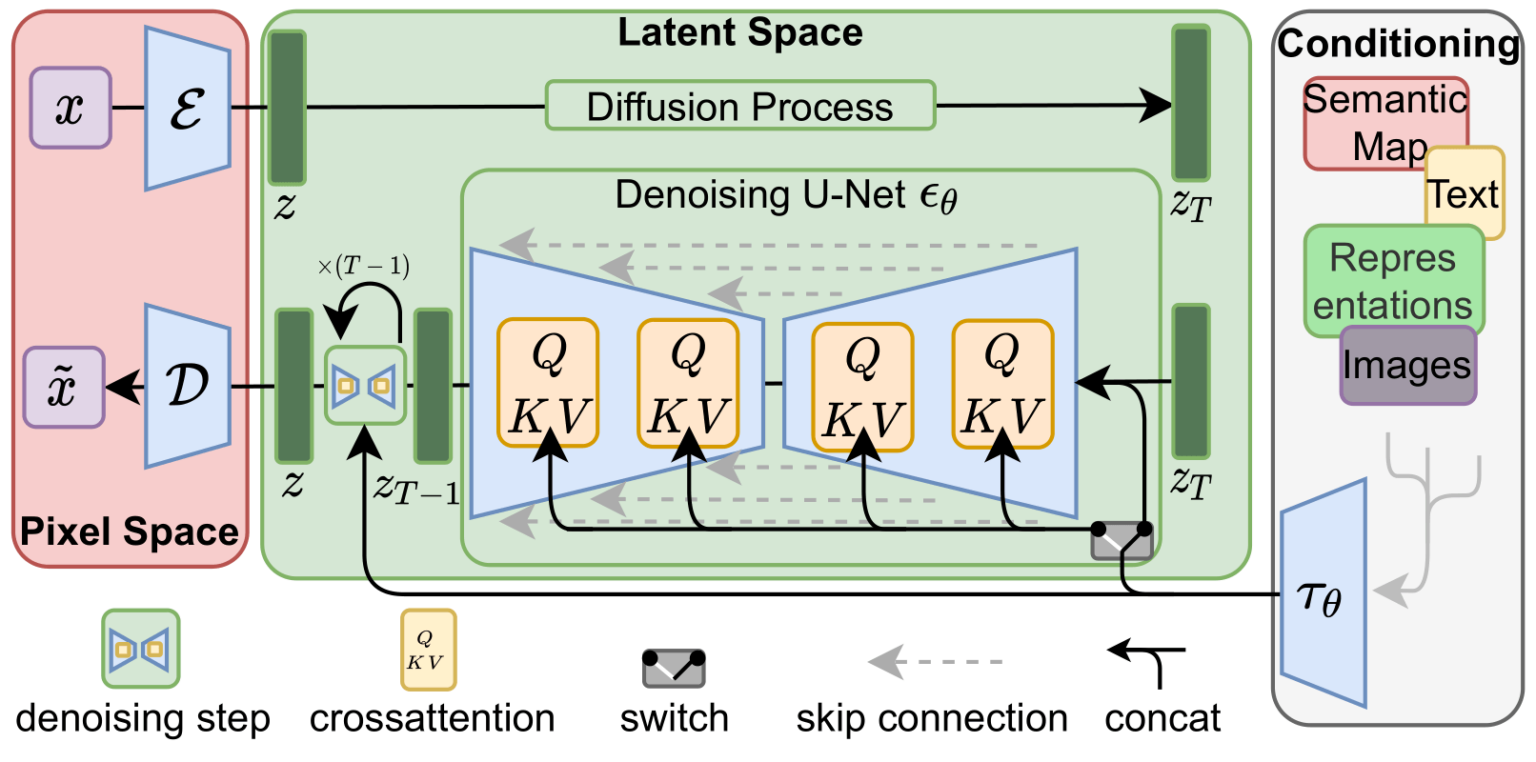
\includegraphics[width=1\linewidth]{article-Figure3-1-1536x762.png}
    \caption{Architectural diagram of a conditional diffusion model. The system operates between Pixel Space (left) and Latent Space (center), with various conditioning inputs (right). The process begins with an encoder ($\epsilon$) mapping input images ($x$) to latent representations ($z$), followed by a forward diffusion process reaching noise level $z_T$. The denoising phase employs a U-Net ($\epsilon_\theta$) with cross-attention mechanisms ($Q$,$K$,$V$) that incorporate conditioning signals ($\tau_\theta$) from text, semantic maps, and other representations. The iterative denoising process transitions from $z_T$ to $z_{T-1}$ and continues until reaching $z$, after which the decoder ($\mathcal{D}$) reconstructs the output image ($\tilde{x}$). Skip connections (dashed arrows) facilitate information flow across the U-Net, while the concatenation operations (black arrows with T-junctions) integrate features at multiple scales.}
    \label{fig:diffusion_architecture}
\end{figure}

\subsection*{1. Denoising Diffusion Probabilistic Models (DDPM)}
\begin{itemize}
  \item \textbf{Generative process:}  
    \begin{itemize}
      \item Forward: add Gaussian noise in $T$ small steps to a clean image $x_0$, producing noisy $x_t$.  
      \item Reverse: learn a denoiser $\varepsilon_\theta(x_t,t)$ to recover $x_{t-1}$ from $x_t$.  
      \item Objective: minimize 
        \[
          \mathcal{L}_{\text{DDPM}} = \mathbb{E}_{x,\varepsilon\sim\mathcal{N}(0,1),t}\bigl[\|\varepsilon - \varepsilon_\theta(x_t,t)\|^2\bigr].
        \]
    \end{itemize}
  \item \textbf{Drawbacks:}
    \begin{itemize}
      \item Operates in high-dimensional \emph{pixel} space, so each sampling step requires a full UNet pass on the full image.
      \item Typically uses hundreds to thousands of timesteps: inference is slow (e.g.\ 50 K samples take ~5 days on A100) and training can cost \(\sim\)150–1000 V100-GPU-days.
      \item Requires large datasets to learn pixel-space noise-removal.
    \end{itemize}
\end{itemize}

\subsection*{2. Stable Diffusion (Latent Diffusion Model, LDM)}
\begin{itemize}
  \item \textbf{Key idea:} Perform diffusion not in pixels but in a learned \emph{latent} space of a powerful autoencoder.  
  \item \textbf{Two-stage training:}
    \begin{enumerate}
      \item \emph{Perceptual compression stage:}  
        Train an autoencoder $(E,D)$ (with a small KL- or VQ-regularization) to map $x\!\in\!\mathbb{R}^{H\times W\times3}$ to $z\!\in\!\mathbb{R}^{h\times w\times c}$, where $h=H/f$ (e.g.\ $f=4$).
      \item \emph{Latent diffusion stage:}  
        Train a time-conditional UNet $\varepsilon_\theta(z_t,t)$ to denoise $z_t$ back to $z_{t-1}$, minimizing
        \[
          \mathcal{L}_{\mathrm{LDM}} 
          = \mathbb{E}_{z,\varepsilon,t}\bigl[\|\varepsilon - \varepsilon_\theta(z_t,t)\|^2\bigr]
        \]
        where $z_0=E(x)$ and $z_t$ follows the fixed forward diffusion in latent space.
    \end{enumerate}
  \item \textbf{Efficiency gains:}
    \begin{itemize}
      \item Latent dimensionality is much lower ($h\!\times\!w\!\ll\!H\!\times\!W$), so each denoising step is far cheaper.
      \item Overall training and sampling speed can improve by \(\sim\!3\times\) or more compared to a pixel DDPM .
    \end{itemize}
  \item \textbf{Conditional generation:}
    \begin{itemize}
      \item Incorporate arbitrary conditioning (e.g.\ text) via a domain encoder $\tau_\phi(y)$ plus cross-attention layers in the UNet backbone
      \item At inference: use classifier-free guidance to trade off fidelity vs.\ adherence to $y$.
    \end{itemize}
  \item \textbf{Decoding:} After denoising to $\hat z_0$, reconstruct $\hat x = D(\hat z_0)$.
\end{itemize}

\subsection*{3. Main Differences DDPM vs.\ Stable Diffusion}
\begin{itemize}
  \item \textbf{Operational domain:}  
    DDPM acts on full RGB pixels; SD acts on compressed latents.  
  \item \textbf{Compute \& memory:}  
    DDPM: high FLOPs/GPU memory per step (full image).  
    SD: lower cost per step (small latent), faster sampling & training.
  \item \textbf{Model structure:}  
    DDPM = single UNet over pixels.  
    SD = (pretrained autoencoder) + latent UNet + optional text encoder + cross-attention.
  \item \textbf{Flexibility:}  
    SD reuses one autoencoder for many tasks, and its cross-attention easily supports multi-modal conditioning (text, layouts, masks), whereas DDPMs typically use simple concatenation or class conditioning.
  \item \textbf{Quality vs.\ efficiency trade-off:}  
    SD finds a near-optimal balance between compression and detail preservation by choosing $f$ (often $4$–$8$) .
\end{itemize}

\subsection*{1. Comparing Stable Diffusion (SD) vs.\ SDXL}
\begin{itemize}
  \item \textbf{Overall pipeline:} Both SD and SDXL are Latent Diffusion Models (LDMs) that operate in a compressed latent space via a pretrained VAE $(E,D)$, apply a time-conditional UNet for denoising, then decode back to pixel space.  
  \item \textbf{UNet backbone size:}  
    \begin{itemize}
      \item \emph{SD (v1.4/2.1)}: $\sim$1 B parameters in the U-Net denoiser.  
      \item \emph{SDXL 1.0}: a \emph{three times larger} UNet backbone (≈3.5 B parameters), achieved by adding more attention blocks and increasing the hidden dimensionality }.
    \end{itemize}
  \item \textbf{Text conditioning:}
    \begin{itemize}
      \item \emph{SD}: single CLIP-style text encoder, cross-attention at each UNet layer.  
      \item \emph{SDXL}: \emph{two} text encoders (e.g.\ OpenCLIP-ViT/G & CLIP-ViT/L), allowing dual-prompt or more expressive guidance; cross-attention uses the concatenated context from both encoders.
    \end{itemize}
  \item \textbf{Aspect ratios \& resolutions:}
    \begin{itemize}
      \item \emph{SD}: trained primarily at square 512×512 (later 768×768) resolutions.  
      \item \emph{SDXL}: trained on \emph{multiple aspect ratios} (e.g.\ 1:1, 3:2, 2:3, 1:2, 2:1) to retain fidelity across portrait/landscape formats .
    \end{itemize}
  \item \textbf{Refinement stage:}  
    \begin{itemize}
      \item \emph{SD}: single diffusion denoiser.  
      \item \emph{SDXL}: includes an \emph{optional refiner} UNet, applied post-hoc in an img2img fashion to sharpen and add fine details to the base SDXL .
    \end{itemize}
  \item \textbf{Sampling efficiency:}  
    \begin{itemize}
      \item Larger models slow down per-step inference, but SDXL’s improved capacity often requires fewer steps for equivalent or better quality.  
      \item A distilled “XL Turbo” variant further reduces the number of denoising steps needed.
    \end{itemize}
\end{itemize}

\subsection*{2. Explanation of the Stable Diffusion Pipeline Diagram}
A canonical SD diagram (cf.\ Fig.~\ref{fig:sd_pipeline}) breaks down into:
\begin{enumerate}
  \item \textbf{VAE Stage:}  
    \begin{itemize}
      \item \emph{Encoder $E$:} maps pixel image $x\in\mathbb{R}^{H\times W\times3}$ to latent $z=E(x)\in\mathbb{R}^{h\times w\times c}$.  
      \item \emph{Decoder $D$:} reconstructs $\tilde x=D(z)$ for training the VAE; frozen at diffusion-training time.
    \end{itemize}
  \item \textbf{Forward diffusion (latent):}  
    \[
      z_t \;=\;\sqrt{\bar\alpha_t}\,z_{t-1}\;+\;\sqrt{1-\bar\alpha_t}\,\epsilon,\quad \epsilon\!\sim\!\mathcal{N}(0,I),
    \]
    gradually corrupting $z$ with Gaussian noise over $T$ timesteps.
  \item \textbf{Denoising UNet $\varepsilon_\theta(z_t,t,y)$:}  
    \begin{itemize}
      \item \emph{Time embedding} encodes $t$.  
      \item \emph{Cross-attention} layers inject conditioning (text embeddings or other) into intermediate UNet blocks.  
      \item \emph{Skip connections} shuttle high-resolution details from encoder to decoder paths.  
      \item Predicts noise estimate $\hat\epsilon$ to recover $z_{t-1}$ from $z_t$.
    \end{itemize}
  \item \textbf{Reverse diffusion sampling:}  
    Iteratively apply the learned denoiser, optionally with classifier-free guidance, to obtain $\hat z_0$.
  \item \textbf{Reconstruction:}  
    Decode $\hat z_0$ back to pixel space: $\hat x = D(\hat z_0)$, yielding the final generated image.
\end{enumerate}

\chapter{Project Related in-depth knowledge}

\section{Problem}
Text
\section{Solution}

\section{Data}

\section{Data preprocessing}

\section{Models}

\subsection{Vision Language Models}

\subsection{Diffusion Models}

\subsection{Vision Transformer}


\section{Training}
\subsection{Parameters}
\subsection{Loss Functions}


\section{Results}









\chapter{Glossary of Terms}

\section{Explainability and Fairness}

\begin{description}
  \item[Explainable AI (XAI):] Methods and techniques that allow human users to understand, trust, and effectively manage AI systems. In computer vision, it often aims to explain model predictions.
  \item[Counterfactual XAI:] An explanation that answers "How should the input change to obtain a different classification?" It involves identifying minimal changes to an input that alter the model's prediction.
  \item[Algorithmic Fairness:] The principle and methods aimed at reducing unwanted bias in algorithmic decision-making, ensuring outcomes are equitable across different groups.
  \item[Independence (Algorithmic Fairness):] A notion of fairness where the prediction (or acceptance rate) is independent of group membership.
  \item[Separation (Algorithmic Fairness):] A notion of fairness requiring equal rates of True Positives, False Positives, True Negatives, and False Negatives across different groups.
  \item[Sufficiency (Algorithmic Fairness):] A notion of fairness requiring equal positive and negative predictive values across different groups, meaning given a prediction, the probability of it being true is the same across groups.
\end{description}

\section{Transformers and Language Models}

\begin{description}
  \item[Transformer:] A neural network architecture that relies heavily on self-attention mechanisms to process sequential data, initially developed for natural language processing but adapted for computer vision (Vision Transformers).
  \item[Transformer Encoder:] Part of the original Transformer architecture responsible for processing the input sequence in parallel and generating contextualized representations.
  \item[Transformer Decoder:] Part of the original Transformer architecture responsible for generating the output sequence autoregressively, often utilizing masked attention and cross-attention.
  \item[Self-Attention:] A mechanism within Transformers that allows each element in a sequence to weigh the importance of all other elements in the same sequence when computing its representation.
  \item[Multi-Head Attention:] An extension of self-attention where the attention mechanism is applied multiple times in parallel with different learned linear projections of the input.
  \item[Positional Encoding:] A method used in Transformers to inject information about the position of elements in a sequence, as self-attention is permutation-equivariant.
  \item[Masked Attention:] An attention mechanism used in Transformer Decoders that prevents attention to subsequent positions in the sequence, ensuring autoregressive generation.
  \item[Cross-Attention:] An attention mechanism used in Transformer Decoders (in Encoder-Decoder models) where the queries come from the decoder's sequence and the keys and values come from the encoder's output sequence.
  \item[BERT (Bidirectional Encoder Representations from Transformers):] An encoder-only LLM trained using Masked Language Modeling, focusing on understanding and classifying text.
  \item[GPT (Generative Pre-trained Transformer):] A decoder-only LLM trained using Autoregressive Language Modeling, focusing on generating text.
  \item[Large Language Models (LLMs):] Language models with a very large number of parameters, trained on vast amounts of text data, capable of performing various NLP tasks including text generation.
  \item[Tokenization:] The process of converting text into discrete units (tokens) that can be processed by a language model.
  \item[Decoding Strategies:] Algorithms used to select the next token during the generation process in autoregressive models, examples include Greedy, Beam Search, Multinomial Sampling, Top-K, and Top-P sampling.
\end{description}

\section{Generative Models and Diffusion}

\begin{description}
  \item[Generative AI:] AI models capable of creating new data, such as images, text, or audio, that are similar to the data they were trained on.
  \item[Generative Model:] A model that describes a probability distribution and can sample from it to generate new data points.
  \item[Density Modelling:] The task of learning the underlying probability distribution of a dataset. Generative models often perform this implicitly or explicitly.
  \item[Diffusion Models:] A class of generative models that work by gradually adding noise to data (forward process) and then learning to reverse this process to generate new data from noise (reverse process).
  \item[Forward Diffusion Process:] The process of gradually adding noise to an image over time steps, defined as a Markov chain.
  \item[Reverse Diffusion Process:] The process of gradually removing noise from a noisy image over time steps to generate a clean image, which is learned by the diffusion model.
  \item[Variance Schedule ($\beta_t$):] A sequence of hyperparameters that determine the scale of noise added at each step in the forward diffusion process.
  \item[Denoising:] The task of removing noise from an image; this is what the neural network within a diffusion model learns to do at each step of the reverse process.
  \item[U-Net:] A convolutional neural network architecture commonly used for image-to-image tasks like segmentation and denoising, often employed as the backbone for diffusion models.
  \item[Guidance:] Techniques used to steer the generative process of Diffusion Models towards desired attributes, such as generating images belonging to a specific class or matching a text prompt.
  \item[Classifier Guidance:] A guidance technique for Diffusion Models that uses the gradients of a separate classifier with respect to the image to steer the generation towards a target class.
  \item[Classifier-Free Guidance:] A guidance technique that trains a single Diffusion Model capable of both unconditional and conditional generation, using a weighted combination of the scores from both to achieve guidance.
  \item[Counterfactual Explanations (for image classifiers):] Explanations that show the minimal changes required to an image input to change its classification by a model.
  \item[Universal Guidance:] A guidance framework for Diffusion Models that can incorporate guidance from various modalities (e.g., text prompts, segmentation masks, bounding boxes) using a shared loss function.
  \item[Latent Diffusion Models:] Diffusion Models that operate in a lower-dimensional latent space learned by an autoencoder, rather than directly in the pixel space, making them more efficient for high-resolution images.
  \item[Stable Diffusion:] A popular latent diffusion model capable of high-quality text-to-image generation and other image manipulation tasks.
\end{description}

\section{Self-Supervised and Multimodal Learning}

\begin{description}
  \item[Self-Supervised Learning (SSL):] A machine learning paradigm where a model learns from unlabelled data by training on "pretext tasks" where the labels are derived automatically from the data itself.
  \item[Pretext Tasks:] Tasks used in self-supervised learning to train a model without requiring human annotations, such as predicting missing parts of an image or learning spatial relationships.
  \item[Contrastive Learning:] An SSL approach that learns representations by pulling together embeddings of augmented versions of the same image (positives) and pushing apart embeddings of different images (negatives).
  \item[MAE (Masked Autoencoders):] An SSL approach that trains a Vision Transformer to reconstruct missing patches of an image.
  \item[DINO (Self-supervised Vision Transformers):] An SSL approach that trains Vision Transformers by self-distillation, where a "student" network learns from a "teacher" network of the same architecture.
  \item[Multimodal Learning:] Machine learning that processes and relates information from multiple modalities, such as combining visual and textual data.
  \item[CLIP (Contrastive Language--Image Pre-training):] A multimodal model trained to connect images and text using a contrastive objective, enabling zero-shot image classification and text-to-image generation.
  \item[Visual Question Answering (VQA):] A multimodal task where a model is given an image and a natural language question about the image and must provide a natural language answer.
  \item[Visual Reasoning:] Multimodal tasks requiring deeper understanding and inference about the spatial and semantic relationships between objects in an image based on text queries.
  \item[Image-Text Contrastive (ITC) Loss:] A loss function used in multimodal training (like BLIP) to align representations from different modalities (image and text) in a shared embedding space.
  \item[Image-Text Matching (ITM) Loss:] A loss function used in multimodal training (like BLIP) to determine if a given image-text pair is a positive match or a negative mismatch.
  \item[Language Modeling (LM) Loss:] A loss function used in training language models or the text generation component of multimodal models (like BLIP) to predict the next token in a sequence.
  \item[Grounding DINO:] An open-set object detection model that can detect objects based on arbitrary text prompts, combining object detection and language grounding.
  \item[Textual Inversion:] A technique for personalizing generative models (like Stable Diffusion) by learning a new "word" (a text embedding) in the model's vocabulary to represent a specific concept or object from a few example images.
  \item[Zero-shot Classification:] The ability of a model to classify images into categories it has not seen during training, often enabled by multimodal models like CLIP by relating images to text descriptions of categories.
\end{description}

\section{Miscellaneous}

\begin{description}
  \item[Autoregressive:] A property of models that generate sequences one element at a time, conditioning on the previously generated elements.
  \item[Markov Chain:] A stochastic process where the future state depends only on the current state, not on the sequence of events that preceded it. Used to define the forward process in diffusion models.
\end{description}

\afterpage{%
\begin{figure}[p]
    \centering
\includegraphics[width=0.5\paperwidth,height=0.5\paperwidth,keepaspectratio]{Pictures/Mind Map Deep Learning Role Play.png}
\caption{Mind map of the whole course}
    \label{fig:mindmap}
\end{figure}
  \clearpage
}


%
\section{Syntax examples}
\subsection{Cone}
\begin{definition}[Cone]
A set $K \in \R^n$, when $x \in K $ implies $\alpha x \in K$.
\end{definition}
\begin{example}
$S_1^n  \{ X | X=X^n ,\lambda(x) \ge 0\}$\\
A matrix with positive eigenvalues.
\end{example}

\subsubsection{Operations preserving convexity}
\begin{itemize}
\item[Intersection] $C  \cap_{i \in \mathbb{I}}C_i$
\item[Linear map] Let $A : \mathbb{R}^n \to  \R^n$ be a linear map. If $C \in \R^n$ is convex, so is $A(C) = \{Ax \forall x \in C \}$
\item[Inverse image] $A^{-1}(D) = \{ x \in \R |Ax \in D \}$
\end{itemize}

\begin{theorem}[Carathéodory's theorem]
If a point $x \in \R^d$ lies in the convex hull of a set $P$, there is a subset $P'$ of $P$ consisting of $d + 1$ or fewer points such that $x$ lies in the convex hull of $P'$. Equivalently, x lies in an r-simplex with vertices in P.
\end{theorem}

\section{Convex Functions}
\begin{definition}[Convex function]
Let $C \in \R^n$ be convex, $f:C \to \R$ is convex on f if $x,y \in C \times C$. $\forall \alpha \in (0,1)$, $f(\alpha x + (1-\alpha) y) \le f(\alpha x) + f((1-\alpha) y)$
\end{definition}

\begin{remark}
$f$ is convex $\Rightarrow$ $-f$ is concave.
\end{remark}

\section{Support Function}
Take a set $C \in \R^n$, not necessarily convex.The support function is $\sigma_C = \R^n \to \bar{\R}$. $\sigma_C(x) = \sum \{ \langle x,u\rangle  | u \in C\}$.
\includegraphics[scale=0.5]{1_1.png}
\begin{fact}
The support function binds the supporting hyper-plane.
\end{fact}
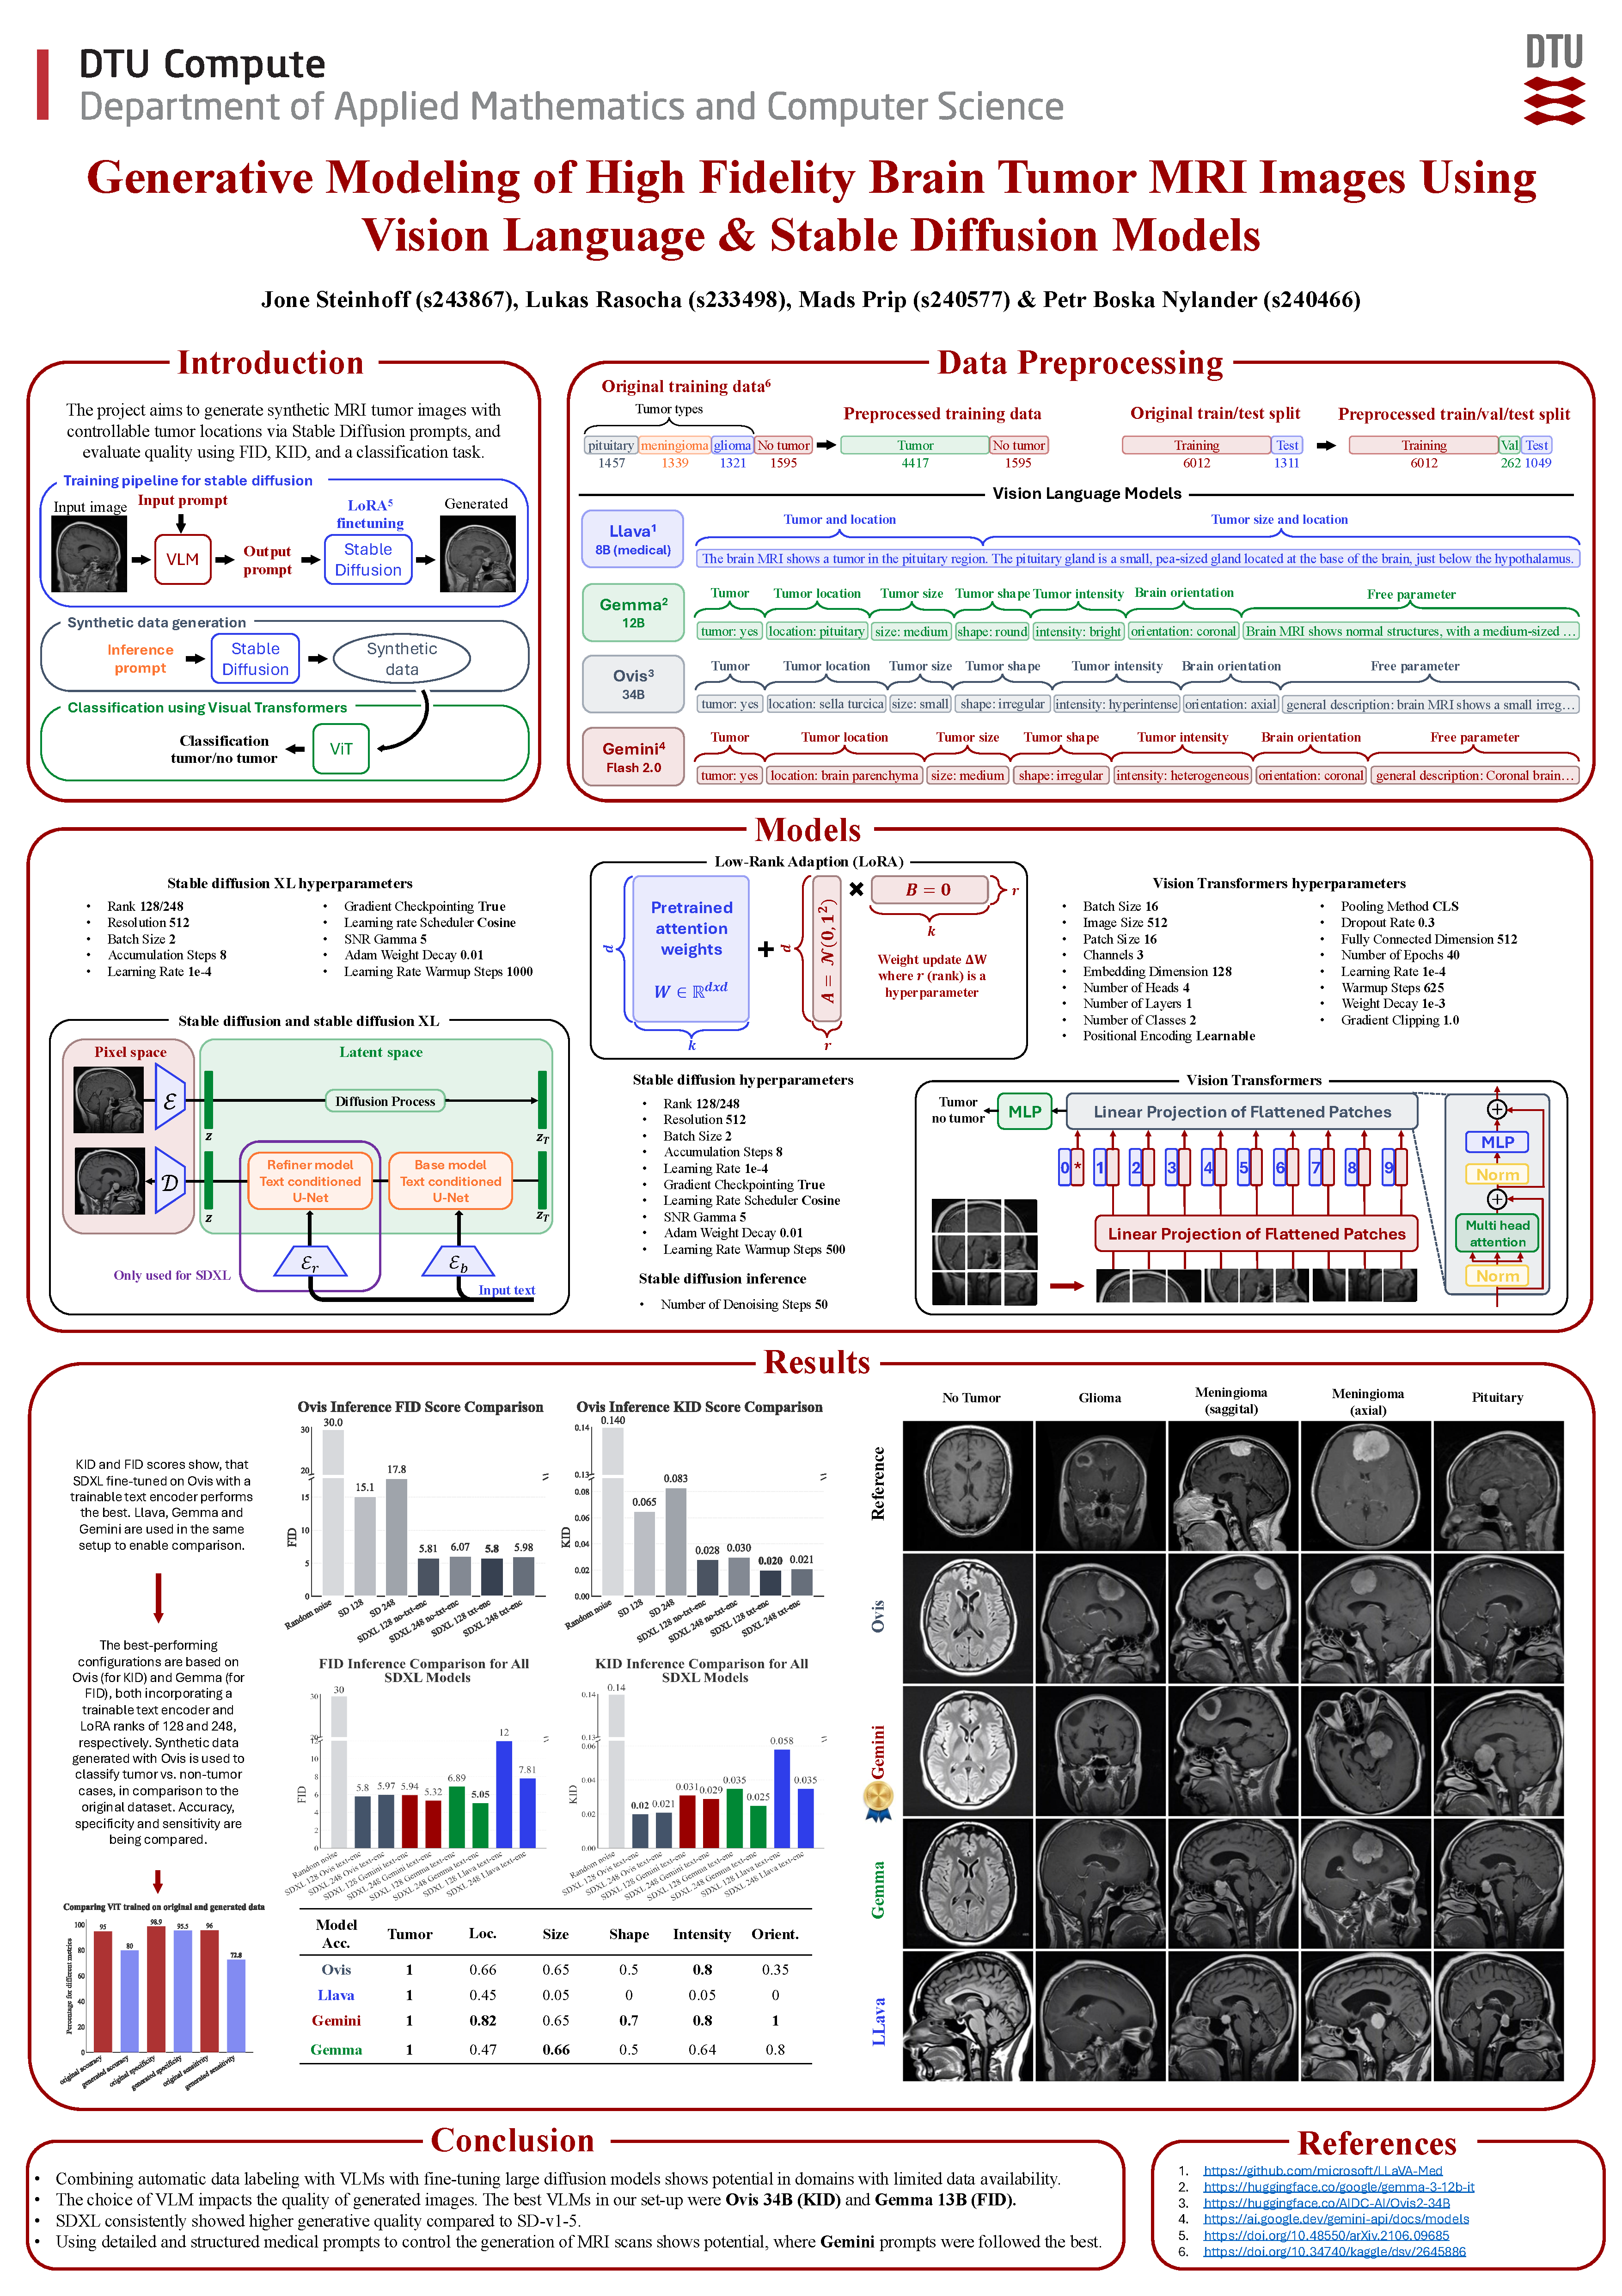
\includepdf[pages=-]{Pictures/final_handin_adlcv.pdf}

\end{document}